% Constructive Approximation development manuscript.
% Publisher template provenance and build: BUILD.md. Draft status: README.md.
\documentclass[pdflatex,sn-mathphys-num]{sn-jnl}
\usepackage{graphicx}
\usepackage{tikz}
\usepackage{amsmath,amssymb,amsfonts}
\usepackage{booktabs}
\usepackage{url}
\theoremstyle{thmstyleone}
\newtheorem{theorem}{Theorem}[section]
\newtheorem{lemma}[theorem]{Lemma}
\newtheorem{proposition}[theorem]{Proposition}
\newtheorem{corollary}[theorem]{Corollary}
\theoremstyle{thmstyletwo}
\newtheorem{remark}[theorem]{Remark}
\newtheorem{definition}[theorem]{Definition}
\hypersetup{bookmarksdepth=2,
 pdftitle={Sharp asymptotics and exact maximizers of the Padua Lebesgue constant},
 pdfauthor={Development manuscript; authors to be supplied}}
\raggedbottom
\begin{document}
\title[Padua Lebesgue constants]{Sharp asymptotics and exact maximizers of the Padua Lebesgue constant}
\author{\fnm{Author details} \sur{to be supplied}}
\affil{\orgname{Affiliation to be supplied}}
\abstract{The Lebesgue constant controls the stability of polynomial interpolation.
For the Padua points of total degree $n$ on the square, we determine its
maximizers and obtain a sharp asymptotic expansion. The maximum is attained
exactly at the two corners outside the interpolation set, for every $n\geq2$.
Writing $N=n+1/2$ and $d=\gamma+\log(8/\pi)$, the expansion is
$\Lambda_n=(4/\pi^2)(\log N+d)^2+\kappa-1/N+O(\log N/N^2)$,
where $\kappa$ is given by a convergent integral. The corner expansion
is analytic: two harmonic sums give the leading square, while a coupled
correction accounts for the constant and the reciprocal term. The global
maximizer proof retains the cancellation lost by a periodic majorant.
It combines quantitative localization for $n\geq320$ with rigorous finite
certificates below that threshold. We describe the certificate implications,
arithmetic dependencies and reproducibility boundary separately from the
analytic asymptotic argument.}
\keywords{Padua points, Lebesgue constant, bivariate interpolation, asymptotic expansion, computer-assisted proof}
\pacs[MSC Classification]{41A05, 41A63, 41A60, 65D05}
\maketitle
\noindent\textbf{Development draft, 7 November 2026.}
Authorship, declarations and a permanent code/data release remain to be
completed. The mathematical exposition has been consolidated around the
corner calculation and the global cancellation comparison.

% CA requires numerical references in alphabetical author order.
% The publisher's sn-mathphys-num style defaults to citation order.
\nocite{MorrowPatterson2026,BialasCiezDeMarchiSuder2026,Mesh2024,BosCaliariDeMarchiVianelloXu2006,BosDeMarchiVianelloXu2007,CaliariDeMarchiSommarivaVianello2008poster,CaliariDeMarchiVianello2005,Computational2008,DeMarchi2022,KolomoitsevLomako2021}
\section{Introduction}\label{sec:introduction}
Polynomial interpolation replaces data at finitely many points by a polynomial.
Its usefulness depends on two questions: how well can polynomials approximate
the function, and how much can interpolation magnify errors in the data?
The Lebesgue constant measures the second effect. If $I_n$ denotes an
interpolation operator and $\Lambda_n=\|I_n\|$, then
\begin{equation}\label{eq:lebesgue-inequality}
 \|f-I_nf\|_\infty\leq (1+\Lambda_n)
       \inf_{p\in\Pi_n}\|f-p\|_\infty.
\end{equation}
The same constant bounds the amplification of uniformly bounded perturbations
of the sampled values. Thus its size has a direct interpretation in both
approximation and numerical stability.

The Padua points are a particularly effective interpolation set on the square.
They contain exactly as many points as the dimension of the space of
polynomials of total degree at most $n$, yet their Lebesgue constants grow
only like the square of a logarithm. Their construction, interpolation
formulas and computational properties have been studied extensively;
see \cite{CaliariDeMarchiVianello2005,BosCaliariDeMarchiVianelloXu2006,
BosDeMarchiVianelloXu2007,Computational2008,DeMarchi2022}.
We consider the following orientation of the points:
\begin{equation}\label{eq:nodes}
 \mathcal P_n=\left\{\left(\cos\frac{j\pi}{n},
                   \cos\frac{k\pi}{n+1}\right):
 0\leq j\leq n,\quad 0\leq k\leq n+1,\quad j+k\ \hbox{even}\right\}.
\end{equation}
Giving the coordinates explicitly avoids differences in the naming of the
Padua families. All statements below refer to \eqref{eq:nodes}.


\begin{figure}[t]
\centering
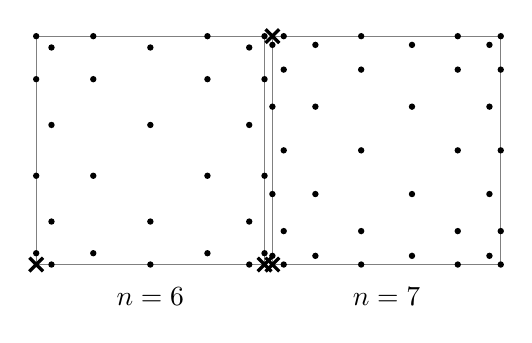
\begin{tikzpicture}[x=1.45cm,y=1.45cm]
\foreach \nn/\mm/\dx in {6/7/0,7/8/3} {
 \begin{scope}[xshift=\dx cm]
  \draw[gray] (-1,-1) rectangle (1,1);
  \foreach \jj in {0,...,\nn} {
   \foreach \kk in {0,...,\mm} {
    \pgfmathtruncatemacro{\parity}{mod(\jj+\kk,2)}
    \ifnum\parity=0
     \fill ({cos(180*\jj/\nn)},{cos(180*\kk/\mm)}) circle (0.028);
    \fi
   }
  }
  \draw[very thick] (-1.06,-1.06)--(-0.94,-0.94)
                    (-1.06,-0.94)--(-0.94,-1.06);
  \ifnum\nn=6
   \draw[very thick] (0.94,-1.06)--(1.06,-0.94)
                     (0.94,-0.94)--(1.06,-1.06);
  \else
   \draw[very thick] (-1.06,0.94)--(-0.94,1.06)
                     (-1.06,1.06)--(-0.94,0.94);
  \fi
  \node[below] at (0,-1.12) {$n=\nn$};
 \end{scope}
}
\end{tikzpicture}
\caption{The Padua points for two consecutive degrees. Dots are interpolation
points; crosses mark the two corners where the Lebesgue function attains
its maximum. The change of orientation depends only on parity.}
\label{fig:padua-nodes}
\end{figure}

Let $L_B$ be the cardinal polynomial associated with $B\in\mathcal P_n$.
The Lebesgue function and its maximum are
\[
 \lambda_n(z)=\sum_{B\in\mathcal P_n}|L_B(z)|,
 \qquad \Lambda_n=\max_{z\in[-1,1]^2}\lambda_n(z).
\]
At an interpolation point the Lebesgue function is exactly one. Away from
the points, its individual cardinal terms can reinforce each other.
For Padua interpolation the largest reinforcement occurs at the two corners
that are not interpolation points. This location was observed numerically
and posed as a question in earlier work
\cite{CaliariDeMarchiSommarivaVianello2008poster,DeMarchi2022}.
Our first result identifies these maximizers exactly.

\begin{theorem}[Location of the maximum]\label{thm:main-location}
For every integer $n\geq2$, the maximum of $\lambda_n$ on the closed square
is attained exactly at
\[
 \begin{cases}
 \{(-1,-1),(1,-1)\},&n\text{ even},\\
 \{(-1,-1),(-1,1)\},&n\text{ odd}.
 \end{cases}
\]
In particular, $\Lambda_n=\Lambda_c(n)$, where
$\Lambda_c(n):=\lambda_n(-1,-1)$.
\end{theorem}

The proof combines an analytic argument, valid for $n\geq320$, with
rigorous finite certificates for the remaining degrees. The certificates
bound the function on regions of the square; they do not infer the maximum
from a collection of sampled values. The analytic argument also uses a
separately certified constant enclosure in its quantitative estimates.
These dependencies are described in Sections~\ref{sec:argmax}
and~\ref{sec:certificates}.

Knowing the location reduces the Lebesgue constant to a single corner
value. Our second result describes that value much more precisely than
its leading growth rate. Write
\begin{equation}\label{eq:main-constants}
 a=\frac2\pi,\qquad d=\gamma+\log\frac8\pi,\qquad
 c_1=ad,\qquad b=2ac_1,\qquad c=c_1^2+\kappa,
\end{equation}
where $\gamma$ is Euler's constant and
\begin{equation}\label{eq:main-kappa}
 \kappa=\frac8\pi\int_0^1 t^2\cot\frac{\pi t}{2}
       \sum_{\substack{\ell\geq1\\\ell\text{ odd}}}
       \frac{1}{\ell(\ell^2-t^2)}\,dt.
\end{equation}
The apparent singularity at $t=1$ is canceled by the cotangent factor;
we justify convergence below.

\begin{theorem}[Sharp corner expansion]\label{thm:main-expansion}
Let $N=n+\tfrac12$. For the points \eqref{eq:nodes}, as $n\to\infty$,
\begin{equation}\label{eq:main-expansion}
 \Lambda_c(n)=\frac4{\pi^2}\log^2N+b\log N+c-\frac1N
            +O\!\left(\frac{\log N}{N^2}\right).
\end{equation}
The constants and the remainder estimate are the same for both parities.
More precisely, a finite constant $C$, independent of $n$, bounds the
absolute remainder by $C\log N/N^2$ for every integer $n\geq2$.
Consequently \eqref{eq:main-expansion} also holds for $\Lambda_n$.
\end{theorem}

The corner expansion is proved entirely analytically. Its global version
uses Theorem~\ref{thm:main-location}, with the computer-assisted dependencies
just described. No numerical fit is used to determine $b$, $c$ or the
coefficient $-1$.

\subsection{What the expansion says}
The dominant term was established by Kolomoitsev and Lomako
\cite{KolomoitsevLomako2021}:
\[
 \Lambda_n=\frac4{\pi^2}\log^2n+O(\log n).
\]
Our expansion resolves the terms hidden in that error, down to an error
smaller than $1/n$. Its leading part can be written more suggestively as
\[
 \left[\frac2\pi\left(\log N+\gamma+\log\frac8\pi\right)\right]^2
       +\kappa-\frac1N.
\]
The square comes from two one-dimensional harmonic sums. The constant
$\kappa$ measures the defect in replacing the coupled two-dimensional
corner formula by their product. The term $-1/N$ records the first
interaction between the boundary corrections and the displacement of the
two meshes. Centering at $N=n+1/2$ makes that interaction visible: a
logarithmic first correction present in the coordinate $n+1$ cancels
against the change of variable. Section~\ref{sec:asym} explains this
cancellation before turning to its estimates.

\subsection{The idea behind the maximizer proof}
A direct comparison of all the absolute cardinal terms hides useful
cancellation. Instead, we express the physical Lebesgue function as a
periodic envelope minus a nonnegative defect. The envelope is easier
to estimate. The defect measures the cancellation that is lost when one
passes to that envelope. Near a competing corner the envelope alone is
not enough: retaining the defect is what gives a strict comparison with
$\Lambda_c(n)$.

There are two different geometric tasks. Away from the two maximizing
corners, one needs a uniform positive gap. Near either maximizing corner,
no such gap can exist, because the function is continuous and equals
$\Lambda_c(n)$ at the corner itself. There we prove a strict quadratic
loss in angular coordinates. Together these arguments explain both the
maximum value and its entire equality set. The finite certificates follow
the same distinction: region bounds away from the corners, and a local
strictness argument at the corners.

\subsection{Related work and organization}
The Padua construction and its relation to generating curves and polynomial
ideals are developed in
\cite{BosCaliariDeMarchiVianelloXu2006,BosDeMarchiVianelloXu2007}.
The survey \cite{DeMarchi2022} records the corner-location question, and
\cite{BialasCiezDeMarchiSuder2026} studies geometric features of Lebesgue
functions, including numerical information about local maxima.
These questions should be distinguished from the exact global equality
set in Theorem~\ref{thm:main-location}.

Rigorous evaluation by polynomial meshes has an important earlier
foundation. Bia{\l}as-Cie{\.{z}}, Kenne, Sommariva and Vianello
\cite{Mesh2024} give certified mathematical discretization bounds for
Lebesgue constants on several domains and include Padua examples.
Such bounds control the discretization error; interval evaluation must
also control arithmetic error when they are used as numerical certificates.
Our finite completion uses strict exclusion and local corner estimates
to determine an equality set, rather than an approximation to the norm
alone. We do not claim that rigorous mesh bounds originate here.

For the related Morrow--Patterson points, Beberok, Bia{\l}as-Cie{\.{z}}
and De Marchi \cite{MorrowPatterson2026} prove quadratic growth of the
Lebesgue constant. The two node families have different stability
behavior, and their extremum questions are separate.

We first establish the exact cardinal normalization and the corner
representation. We then derive the sharp expansion, explain the geometric
comparison giving the maximizers, and describe the finite certificates.
Detailed quadrature, row and localization estimates are collected in
appendices so that the main argument can be read without following every
constant calculation.

\section{The interpolation operator and its normalization}\label{sec:preliminaries}
Put $Q=[-1,1]^2$ and let $\Pi_n$ be the real polynomials of total degree
at most $n$. Here $\delta_{AB}$ is one if $A=B$ and zero otherwise.
The cardinal polynomials satisfy $L_B(A)=\delta_{AB}$ for
$A,B\in\mathcal P_n$, and
\[
 I_nf(z)=\sum_{B\in\mathcal P_n} f(B)L_B(z).
\]
The triangle inequality gives $\|I_n\|\leq\max_Q\lambda_n$; equality
follows by prescribing at the nodes the signs of the cardinal values
at a maximizing point and extending these finitely many values
continuously to $Q$. This proves the operator-norm interpretation used
in \eqref{eq:lebesgue-inequality}.

We use the Chebyshev polynomials $T_r(\cos t)=\cos(rt)$. Write
$\theta_j=j\pi/n$, $\phi_k=k\pi/(n+1)$ and
\[
 \varepsilon_j=\begin{cases}1/2,&j=0,n,\\1,&\text{otherwise},\end{cases}
 \qquad
 \eta_k=\begin{cases}1/2,&k=0,n+1,\\1,&\text{otherwise},\end{cases}
 \qquad w_{jk}=\frac{2\varepsilon_j\eta_k}{n(n+1)}.
\]
For the kernel formula below, set $\nu_0=1$ and $\nu_r=2$ for $r>0$;
these are the mode multiplicities. Define
\[
 K_n(z,B)=\sum_{p+q\leq n}\nu_p\nu_q
 T_p(z_1)T_p(B_1)T_q(z_2)T_q(B_2).
\]

\begin{lemma}[Cardinal kernel]\label{lem:cardinal-kernel}
The set $\mathcal P_n$ is unisolvent for $\Pi_n$, and for
$B=(\cos\theta_j,\cos\phi_k)\in\mathcal P_n$,
\begin{equation}\label{eq:cardinal-kernel}
 L_B(z)=w_{jk}\bigl[K_n(z,B)-T_n(z_1)T_n(B_1)\bigr].
\end{equation}
In particular the coefficient of the highest first-coordinate mode is
one.
\end{lemma}
\begin{proof}
For $M\geq1$ let
\[
 Q_M(g)=\frac1M\sum_{j=0}^M{}'g(j\pi/M),
\]
where the prime gives weight $1/2$ to each endpoint. Finite geometric
sums show that $Q_M(\cos rt)=0$ for $1\leq r\leq2M-1$ and
$Q_M(1)=Q_M(\cos2Mt)=1$. Consequently
\[
 Q_M(\cos pt\cos rt)=\delta_{pr}h_p^{(M)},\qquad
 h_p^{(M)}=\begin{cases}1,&p=0,M,\\1/2,&0<p<M.\end{cases}
\]
Multiplication by $(-1)^j$ sends the mode $p$ to $M-p$ on this grid.
In the checkerboard scalar product the identity
$2\mathbf1_{j+k\,\mathrm{even}}=1+(-1)^{j+k}$ splits the Gram matrix
of the modes $T_p(x)T_q(y)$, $p+q\leq n$, into a tensor product part
and an alternating part. The alternating part could be nonzero only
if $p+r=n$ and $q+s=n+1$. Their sum contradicts
$(p+q)+(r+s)\leq2n$, so that part vanishes.
The Gram matrix is therefore diagonal and positive, with diagonal
$h_p^{(n)}h_q^{(n+1)}$.

There are $(n+1)(n+2)/2$ checkerboard points, the same number as the
modes. The square evaluation matrix is invertible, proving unisolvence.
The inverse Gram coefficients are $\nu_p\nu_q$ except at $(p,q)=(n,0)$,
where the coefficient is one. The discrete reproducing kernel, multiplied
by $w_{jk}$, therefore has the cardinal values and gives
\eqref{eq:cardinal-kernel}.
\end{proof}

The same correction appears in the angular kernel
\begin{equation}\label{eq:angular-kernel}
 G_n(u,v)=\sum_{p+q\leq n}\nu_p\nu_q\cos(pu)\cos(qv)-\cos(nu).
\end{equation}
At a corner it gives the exact signed row sums; in the interior its
reflections give the cancellation comparison. Thus the two arguments
start from one normalized kernel.



The two nonnode corners in Theorem~\ref{thm:main-location} have equal
Lebesgue values by symmetry. For even $n$, reflection in the first
coordinate sends $j$ to $n-j$ and preserves the checkerboard. For odd
$n$, reflection in the second coordinate sends $k$ to $n+1-k$ and
preserves it. Uniqueness of interpolation carries these symmetries to
the cardinal polynomials and hence to $\lambda_n$.

\begin{remark}
All formulas involving trigonometric quotients are interpreted by their
continuous polynomial limits at removable singularities. The maximization
and certificate domains include all nodes, edges and collisions of angular
coordinates.
\end{remark}

\section{The corner value: from exact rows to the first correction}
\label{sec:corner}

At a corner the absolute cardinal kernel becomes a positive Cauchy sum.
Its two meshes have sizes $n$ and $n+1$. The equal-mesh reference gives
the leading square; the mesh displacement supplies the constant defect
and the first correction.
Put $m=n+1$ and, for the rest of this section, write
\[
 \theta_j=j\pi/n,\quad \phi_k=k\pi/m,\qquad
 \varepsilon_j=\begin{cases}1/2,&j=0,n,\\1,&0<j<n,\end{cases}
 \quad \eta_k=\begin{cases}1/2,&k=0,m,\\1,&0<k<m.\end{cases}
\]
Every unspecified constant below is independent of $n\geq2$ and of the
row indices in their stated ranges. Set $A(z)=a(\log z+d)$, with the
constants in \eqref{eq:main-constants}.


The principal notation for this section is collected below. Row indices
and all implied constants have the ranges stated in the formulas.
\begin{center}
\begin{tabular}{@{}p{0.36\linewidth}p{0.58\linewidth}@{}}
\toprule
Symbol & Meaning\\
\midrule
$m=n+1$, $N=n+1/2$ & unequal mesh size and midpoint degree\\
$\theta_j$, $\phi_k$; $\varepsilon_j$, $\eta_k$ & angular nodes and endpoint half weights\\
$a,d,A(z)=a(\log z+d)$ & constants of \eqref{eq:main-constants} and logarithmic model\\
$\mathcal D_n$; $w(x),B(x)$ & diamond kernel; cotangent functions, with both poles removed from $B$\\
$x=r/m$, $s=m-r$ & position and complementary distance of row $r$\\
$T_{n,r},V_n,D_{m,r},\mathcal H_m$ & cotangent row sum, smooth sum, digamma row and its aggregate\\
$H_k=\sum_{j=1}^k1/j$ & harmonic numbers\\
\bottomrule
\end{tabular}
\end{center}
The product mesh size used in Section~\ref{sec:argmax} is instead
$\mathsf N=nm$.

\subsection{An exact row formula}
For $u\ne v$ let $f(u,v)=(1+\cos v)/|\cos u-\cos v|$. We first obtain
\begin{equation}\label{cu:positive}
 \Lambda_c(n)=\frac4{nm}
 \sum_{\substack{0\leq j,k\leq n\\j+k\text{ odd}}}
       \varepsilon_j\eta_k f(\theta_j,\phi_k)+\frac1m.
\end{equation}
To see this directly from \eqref{eq:cardinal-kernel}, define
$\mathcal{D}_n(u,v)=\sum_{|p|+|q|\leq n}\mathrm e^{\mathrm i(pu+qv)}$. Grouping positive and negative frequencies in each coordinate gives
\[
 \mathcal D_n(u,v)=\sum_{\substack{p,q\geq0\\p+q\leq n}}
       \nu_p\nu_q\cos(pu)\cos(qv)=G_n(u,v)+\cos(nu).
\]
For $B=(\cos\theta_j,\cos\phi_k)$ and $z=(-1,-1)$,
$T_p(-1)=(-1)^p$ therefore gives
$K_n(z,B)=\mathcal D_n(\pi-\theta_j,\pi-\phi_k)$.
Set $j'=n-j$ and $k'=m-k$. Then
$\pi-\theta_j=\theta_{j'}$, $\pi-\phi_k=\phi_{k'}$,
$(-1)^{n+j}=(-1)^{j'}$, and \eqref{eq:cardinal-kernel} becomes
\[
 L_{jk}(-1,-1)=w_{jk}
 \{\mathcal D_n(\theta_{j'},\phi_{k'})-(-1)^{j'}\}
 =w_{jk}G_n(\theta_{j'},\phi_{k'}).
\]
The reflection changes even checkerboard parity to odd and preserves
the endpoint weights. This is the link between the interpolation kernel
and the positive corner sum. With
$u_+=(u+v)/2$, $u_-=(v-u)/2$, finite geometric sums give
\[
 \mathcal{D}_n(u,v)=\frac{\sin((n+1)u_+)\sin((n+1)u_-)+\sin(nu_+)\sin(nu_-)}
                  {\sin u_+\sin u_-}.
\]
Indeed $(p,q)\mapsto(p+q,q-p)$ takes the diamond into the square
$[-n,n]^2$ with equal coordinate parity; summing its two parity classes
gives the displayed product. Quotients at zero denominators have their
continuous polynomial values. Reflection of node indices about either
nonnode corner turns the checkerboard odd and leaves its weights unchanged.
The corresponding Lebesgue sum is therefore
$\sum_{j+k\text{ odd}}2\varepsilon_j\eta_k
 |\mathcal{D}_n(\theta_j,\phi_k)-(-1)^j|/(nm)$.
For distinct mesh angles, the product-to-sum identities are
\[
 \sin(tu_+)\sin(tu_-)=\tfrac12\{\cos(tu)-\cos(tv)\},
 \qquad \sin u_+\sin u_-=\tfrac12(\cos u-\cos v).
\]
The four mesh cosine values are
\[
 \begin{gathered}
 \cos(n\theta_j)=(-1)^j,\quad
 \cos(m\theta_j)=(-1)^j\cos\theta_j,\\
 \cos(m\phi_k)=(-1)^k,\quad
 \cos(n\phi_k)=(-1)^k\cos\phi_k.
 \end{gathered}
\]
Since $j+k$ is odd, the numerator of $\mathcal D_n$ is
$\tfrac12(-1)^j(2+\cos\theta_j+\cos\phi_k)$.
Thus
\[
 \mathcal{D}_n(\theta_j,\phi_k)=(-1)^j
       \frac{2+\cos\theta_j+\cos\phi_k}{\cos\theta_j-\cos\phi_k},
 \qquad |\mathcal{D}_n(\theta_j,\phi_k)-(-1)^j|=2f(\theta_j,\phi_k).
\]
Coprimality of $n,m$ leaves only the collisions $(0,0)$ and $(n,m)$.
The odd checkerboard excludes the first. At the second,
$\mathcal{D}_n(\pi,\pi)=(-1)^n(2n+1)$, so the corrected absolute value $2n$
with weight $1/(2nm)$ contributes $1/m$. The other entries with $k=m$
vanish. This proves \eqref{cu:positive} and the equality of the two
nonnode corner values. The node corners have value one by cardinality.
For $n=2$, the nonzero weighted summands
$\varepsilon_j\eta_k f(\theta_j,\phi_k)$ at
$(j,k)=(0,1),(1,0),(1,2),(2,1)$ are respectively
$3/2,1,1,1/2$. Formula~\eqref{cu:positive} gives
$\Lambda_c(2)=(4/6)(3/2+1+1+1/2)+1/3=3$.


On row $k=r$ the checkerboard condition fixes $j\equiv1-r\pmod2$,
so $(-1)^j$ is constant along the row. The sign of the denominator
therefore determines its positive samples, making \eqref{cu:positive}
one dimensional. Introduce
\begin{equation}\label{cu:wB}
 w(x)=\cot(\pi x/2),\qquad
 B(x)=\cot(\pi x)-\frac1{\pi x}+\frac1{\pi(1-x)}.
\end{equation}
Both poles have been removed from $B$; it is $C^\infty$ across $[0,1]$,
with $B(0)=1/\pi$, $B(1)=-1/\pi$.
For example, with $\operatorname{sinc}z=\int_0^1\cos(tz)\,dt$,
\[
 \cot z-1/z=-z\,
 \frac{\int_0^1t^2\operatorname{sinc}(tz)\,dt}{\operatorname{sinc}z}.
\]
The denominator is nonzero near zero; differentiation of the finite
integral proves the smooth extension after subtracting the pole.
Reflection gives the extension at the other endpoint.
 For $1\leq r<m$ put
$x=r/m$, $s=m-r$, $\alpha_r=(1-x)/2$ and
\[
 T_{n,r}=\sum_{\ell=0}^{r-1}\cot\frac{\pi(\ell+\alpha_r)}n,
 \qquad V_n=\sum_{r=1}^{m-1}w(r/m)
                    \sum_{\ell=0}^{r-1}B((\ell+\alpha_r)/n).
\]
We define the digamma function $\psi$ by its convergent harmonic series:
\begin{equation}\label{cu:psi}
 \psi(z)=-\gamma+\sum_{k=0}^\infty
          \left(\frac1{k+1}-\frac1{k+z}\right),\qquad z>0,
\end{equation}
Telescoping this series gives
\[
 \psi(z+1)-\psi(z)=1/z,\qquad
 \psi(k+1)=H_k-\gamma,\qquad
 \psi(R+1/2)=\psi(1/2)+2H_{2R}-H_R,
\]
where $H_k=\sum_{j=1}^k1/j$ and $k,R$ are positive integers.
The bounds and half-integer values used below are proved in
Section~\ref{sec:asym}. In particular \eqref{cu:psi-est} gives
$H_k=\log k+\gamma+1/(2k)+O(k^{-2})$ by applying it at $k+1$.

Set
\begin{equation}\label{cu:D}
 D_{m,r}=\psi(r+\alpha_r)+\psi(s-\alpha_r)-\psi(m-\alpha_r)-\psi(\alpha_r),
 \qquad \mathcal H_m=\frac4{\pi m}\sum_{r=1}^{m-1}w(r/m)D_{m,r}.
\end{equation}
We claim the exact identities
\begin{equation}\label{cu:exact}
 \Lambda_c(n)=1-\frac{2n}{m}+\frac4{nm}\sum_{r=1}^{m-1}w(r/m)T_{n,r}
       =-1+\frac2m+\mathcal H_m+\frac{4V_n}{nm}.
\end{equation}
We now write row $k$ of \eqref{cu:positive} as $r$; its entries are
$|F_r(\theta_j)|$. Extend a row periodically
and sample its $n$ indices $j\equiv1-r\pmod2$ modulo $2n$. For
$v=r\pi/m$ its signed entries satisfy
\[
 F_r(u):=\frac{1+\cos v}{\cos u-\cos v}
   =\frac{w(r/m)}2\left(\cot\frac{v-u}{2}+\cot\frac{v+u}{2}\right),
 \qquad \sum_jF_r(j\pi/n)=n.
\]
The cotangent form uses
\[
 \begin{aligned}
 \cot A+\cot B&=\frac{\sin(A+B)}{\sin A\sin B},\\
 2\sin\frac{v-u}{2}\sin\frac{v+u}{2}&=\cos u-\cos v,\\
 \cot(v/2)\sin v&=1+\cos v.
 \end{aligned}
\]
The periodic row sum follows from
$\sum_{\ell=0}^{n-1}\cot(z+\ell\pi/n)=n\cot(nz)$, the logarithmic
derivative of the finite sine product; its right hand cotangent here is
$\tan(v/2)$. The positive samples have representatives
$j=-r+1,-r+3,\ldots,r-1$, since $r-1<nr/m<r$.
Their sum is $P_r=w(r/m)T_{n,r}$, by symmetry and the substitution
$j=r-1-2\ell$. Thus the absolute periodic row is $2P_r-n$.
Folding back to $0\leq j\leq n$ divides by two and produces exactly
$\varepsilon_j$. The folded interior row therefore contributes
$(4/(nm))\eta_r(2P_r-n)/2$ to the corner sum. For $r=0$ the periodic row is $n^2$, since the derivative
of the same cotangent identity gives
$\sum_{\ell=0}^{n-1}\csc^2((\ell+1/2)\pi/n)=n^2$.
Its weight $\eta_0=1/2$, together with the exceptional $1/m$, yields
$\Lambda_c=1/m+n/m+2\sum_{r=1}^{m-1}(2P_r-n)/(nm)$.
This is the first identity in \eqref{cu:exact}. Finally, removing both
poles in each cotangent and using $\psi(z+1)-\psi(z)=1/z$ gives
$T_{n,r}=nD_{m,r}/\pi+\sum_{\ell<r}B((\ell+\alpha_r)/n)$,
which proves the second identity.

\subsection{The square reference and its mesh defect}
The constant in the answer can be identified before calculating any
first corrections. Define
\[
 L_n=\frac2n\sum_{\substack{1\leq r\leq n\\r\text{ odd}}}
 d_r\csc\frac{r\pi}{2n},\qquad d_r=\begin{cases}1/2,&r=n,\\1,&r<n.\end{cases}
\]
The equal-mesh corner sum is exactly a square:
\begin{equation}\label{cu:square}
 \frac4{n^2}\sum_{\substack{0\leq j,k\leq n\\j+k\text{ odd}}}
 \varepsilon_j\varepsilon_k f(\theta_j,\theta_k)=L_n^2.
\end{equation}
Simultaneous reflection of $j,k$ replaces the numerator by $1-\cos\theta_k$,
so averaging replaces it by one. For $j>k$, put $s=j-k$, $r=j+k$ and
$c_r=\csc(r\pi/(2n))$. Both indices are odd and the denominator is
$2/(c_rc_s)$. The two orders cancel the factor two. For fixed $s<n$,
the values $r=s,2n-s$ have half weight and the intervening values weight
one; their sum after reflection $c_{2n-r}=c_r$ is
$c_s+2\sum_{s<r<n,\ r\text{ odd}}c_r+\boldsymbol1_{n\text{ odd}}c_n$.
The sole pair for $s=n$, when present, has weight $1/4$.
These are precisely the terms in $(\sum_{r\text{ odd}}d_rc_r)^2$,
proving \eqref{cu:square} including its endpoint.

Pairing the midpoints $y_r=(2r-1)\pi/(4n)$ gives, by
$\cot y+\tan y=2\csc(2y)$,
\[
 \begin{aligned}
 L_n&=\frac1n\sum_{r=1}^n\cot y_r\\
    &=a(2H_{2n}-H_n)+a\log(2/\pi)+O(n^{-2})=A(n)+O(n^{-2}),
 \end{aligned}
\]
Here $H_k=\sum_{j=1}^k j^{-1}$. For the second equality, $\cot y-1/y$
is smooth on $[0,\pi/2]$,
its integral is $\log(2/\pi)$, and the midpoint error is $O(n^{-2})$.
The last equality uses $H_k=\log k+\gamma+1/(2k)+O(k^{-2})$;
the reciprocal terms in $2H_{2n}-H_n$ cancel.

We next justify the limiting defect, including the endpoint rows. A
uniform comparison, with $\ell=|j-k|$ odd, is
\begin{equation}\label{cu:deform}
 |f(\theta_j,\phi_k)-f(\theta_j,\theta_k)|
                    \leq\frac{\pi^2n}{2\ell^2}.
\end{equation}
This bound follows from an exact difference. The cases $k=0$ or $j=n$ have zero
difference. Otherwise put $u=\theta_j$, $v_0=\theta_k$, $v_1=\phi_k$,
$\delta=v_0-v_1$, $V=(v_0+v_1)/2$, $S_i=(u+v_i)/2$ and
$Q_i=|u-v_i|/2$. The order of $u,v_i$ is unchanged. Exact subtraction gives
\[
 |f(u,v_1)-f(u,v_0)|=
 \frac{\cos^2(u/2)\sin V\sin(\delta/2)}
      {\sin S_0\sin S_1\sin Q_0\sin Q_1}.
\]
Since $\sin S_i\geq\cos(u/2)\sin(v_i/2)$, the quotient preceding
$\sin(\delta/2)$ and the $Q_i$ factors is at most
$\cot(v_0/2)+\cot(v_1/2)\leq\pi(m-k)/k$.
Here $\sin z\geq2z/\pi$ and $\cos z\leq\pi/2-z$ on $[0,\pi/2]$
suffice. Multiplying by $\sin(\delta/2)\leq\pi k/(2nm)$ gives
$\pi^2(m-k)/(2nm)$. If $k<j$, both $\sin Q_i\geq\ell/n$.
If $k>j$, put $h=n-j$; then
$\sin Q_0\geq\ell/n$, $\sin Q_1\geq[n(\ell-1)+h]/(nm)$ and
$m-k\leq h$. The resulting bound is
$\pi^2nh/[2\ell\{n(\ell-1)+h\}]\leq\pi^2n/(2\ell^2)$,
since $h\leq n$. This proves \eqref{cu:deform}.

Let $\Delta_n$ be $4/(nm)$ times the weighted sum of the differences in
\eqref{cu:deform}. The $k=n$ reference row is zero, so changing its weight
from $\eta_n$ to $\varepsilon_n$ has no effect. Equations
\eqref{cu:positive} and \eqref{cu:square} consequently give
\[
 \Lambda_c(n)-L_n^2=\Delta_n+(1-L_n^2)/m.
\]
The second term tends to zero. For fixed odd $\ell$ and $\sigma=\pm1$,
write $k=j+\sigma\ell$, $t=j/n$. On compact subintervals of $(0,1)$,
the cosine difference factors give uniformly
\[
 \frac{f(\theta_j,\phi_k)-f(\theta_j,\theta_k)}n
 \longrightarrow h_{\sigma,\ell}(t)
 =\frac{w(t)}\pi\left(\frac1{|\sigma\ell-t|}-\frac1\ell\right),
\]
because $\phi_k-\theta_j=\pi(\sigma\ell-t)/m$. Bound
\eqref{cu:deform} controls each normalized summand by $C/\ell^2$.
For fixed $\ell$, the rows with $t$ outside $[\delta,1-\delta]$ therefore
contribute at most $C(\delta+1/n)/\ell^2$; the same bound controls the
omitted limiting integrals. Interior Riemann sums, followed by
$\delta\downarrow0$, give the limit for that offset. The tails over
$\ell>M$ are uniformly bounded by $C\sum_{\ell>M}\ell^{-2}$, so they
may then be removed. Pairing orientations leaves
$1/(\ell-t)+1/(\ell+t)-2/\ell=2t^2/[\ell(\ell^2-t^2)]$.
Thus, on the full integer sequence,
\begin{equation}\label{cu:kappa}
 \Lambda_c(n)-A(n)^2\longrightarrow\kappa
\end{equation}
with exactly the integral \eqref{eq:main-kappa}. Its terms with $\ell\geq3$
converge uniformly up to both endpoints; for $\ell=1$ the zero of $w$ at
one cancels the pole. At zero $t^2w(t)\to0$. This also proves the claimed
continuous extension of the integrand.

\subsection{Uniform summation and the first correction}\label{sec:asym}
To obtain the first correction, we return to \eqref{cu:exact}, keeping
the harmonic and smooth parts together.
One elementary quadrature rule will control all remainders.

\begin{lemma}[Quadrature with endpoint logarithms]\label{cu:quadrature}
Suppose $g$ is continuous on $[0,1]$, twice continuously differentiable
inside, with $|g''(x)|\leq C(x^{-1}+(1-x)^{-1})$ there, and, for
$0<x\leq1/2$,
\[
 |g(x)-g(0)|+|g(1-x)-g(1)|\leq Cx(1+|\log x|).
\]
Then
\[
 \frac1m\sum_{r=1}^{m-1}g(r/m)=\int_0^1g(x)\,dx
       -\frac{g(0)+g(1)}{2m}+O(\log m/m^2).
\]
For $g\in C^2[0,1]$ the error is $O(m^{-2})$; its composite midpoint
rule has the same order.
\end{lemma}
\begin{proof}
On a cell $[u,u+h]$, two integrations by parts give
\[
 \frac h2\{g(u)+g(u+h)\}-\int_u^{u+h}g
 =\frac12\int_u^{u+h}(t-u)(u+h-t)g''(t)\,dt.
\]
For $h=1/m$ the two endpoint cells cost $O(h^2(1+|\log h|))$ by
the assumed moduli. On the others the kernel is at most $h^2/8$,
and $\int_h^{1-h}|g''|=O(\log m)$. For bounded second derivative,
the local error is at most $h^3\|g''\|_\infty/12$. Taylor's formula
at the midpoint gives the corresponding bound $h^3\|g''\|_\infty/24$.
\end{proof}

We also record the elementary estimates used below.
We use the following termwise-differentiation criterion: if a series of
continuously differentiable functions converges at one point of a compact
interval and the series of derivatives converges uniformly there, then
the sum is continuously differentiable and its derivative is that series.
Repeated application is valid when the successive derivative series have
the same property. For \eqref{cu:psi}, reciprocal powers give these uniform
bounds on every compact subinterval of $(0,\infty)$.
Differentiating
\eqref{cu:psi} on compact subsets of $z>0$ gives
\[
 \psi'(z)=\sum_{k\geq0}(z+k)^{-2},\quad
 \psi''(z)=-2\sum_{k\geq0}(z+k)^{-3},\quad
 |\psi''(z)|\leq z^{-2}+2z^{-3}.
\]
The unit-cell trapezoid identity applied to $(z+t)^{-1}$ and integral
comparison for $(z+t)^{-2}$ imply, uniformly for $z\geq1$,
\begin{equation}\label{cu:psi-est}
 \psi(z)=\log z-\frac1{2z}+O(z^{-2}),\qquad
 \psi'(z)=z^{-1}+O(z^{-2}).
\end{equation}
Indeed $\psi(z)=\lim_{K\to\infty}(\log K-\sum_{k<K}(z+k)^{-1})$,
and the trapezoid error is bounded by $\tfrac18\int_0^\infty
2(z+t)^{-3}dt$. This also proves the harmonic estimate used above.
The same series gives
$\psi(1/2)=-\gamma-2\log2$, $\psi'(1/2)=\pi^2/2$.
For the latter value, the classical paired partial fraction
$\pi\cot(\pi z)=z^{-1}+\sum_{k\geq1}((z-k)^{-1}+(z+k)^{-1})$
gives $\sum k^{-2}=\pi^2/6$ by its linear term at zero; removing even
indices gives $4\sum_{k\text{ odd}}k^{-2}=\pi^2/2$.
One short derivation of the partial fraction is the cosine series of
$\cos(zs)$ on $[0,\pi]$: its constant coefficient is
$2\sin(\pi z)/(\pi z)$ and its $k$th coefficient is
$2(-1)^kz\sin(\pi z)/(\pi(z^2-k^2))$. The coefficients are absolutely
summable; evaluating at $s=\pi$ gives the identity. All differentiated
series used here converge locally uniformly away from their poles.

Define the finite, endpoint-regular integrals
\[
 I_1=\int_0^1\left(\frac{w(x)}{1-x}-\frac ax\right)dx,
 \qquad I_2=\int_0^1xw(x)\,dx,\qquad I_B=\int_0^1xw(x)B(x)\,dx.
\]
The next proposition contains the only aggregate calculation needed.
\begin{proposition}\label{cu:aggregate}
There are constants $C_H,C_B$, independent of the degree, such that
\begin{align}
 \mathcal H_m&=A(m)^2+C_H+
       \frac{-a^2\log m+\beta_H}{m}+O(\log m/m^2),\label{cu:H}\\
 \frac{4V_n}{nm}&=C_B+\frac{\beta_B}{n}+O(n^{-2}),\label{cu:V}\\
 \beta_H&=-2-a^2(\gamma+2\log2)-a(I_1+I_2),\notag\\
 C_B&=4\int_0^1w(t)\int_0^tB(x)\,dx\,dt,
 \qquad \beta_B=-a^2+2I_B+aI_2.\notag
\end{align}
\end{proposition}
\begin{proof}
First center the harmonic row at its exact integer and half integer
arguments, before expanding. Taylor's formula gives, uniformly for
$r+s=m$, $x=r/m$, $\alpha=(1-x)/2$,
\begin{equation}\label{cu:center}
 \begin{split}
 D_{m,r}={}&\psi(r+1/2)+\psi(s)-\psi(\alpha)-\psi(m)\\
 &-\frac{r\psi'(r+1/2)+s\psi'(s)-s\psi'(m)}{2m}+O(m^{-2}).
 \end{split}
\end{equation}
In fact the three shifts are respectively $r/(2m),s/(2m),s/(2m)$.
For a shift $h$ at $z$ the error is at most
$h^2\{(z-h)^{-2}+2(z-h)^{-3}\}/2$.
The lower arguments are at least $r$, $3s/4$, $3m/4$, respectively;
hence each error is $O(m^{-2})$, even for $r=1$ or $s=1$.
Since $w(r/m)\leq am/r$, its weighted normalized error is
$O(\log m/m^2)$.

Two summable endpoint sequences must still be retained. Put
$e_r=\psi(r+1/2)-\log r$, $u_r=r\psi'(r+1/2)-1$.
The midpoint rule for $t^{-2}$ on $[r,\infty)$ gives
$\psi'(r+1/2)=1/r+O(r^{-3})$: the local errors sum as
$O(\sum_{k\geq0}(r+k)^{-4})$. Integration from infinity, using
\eqref{cu:psi-est}, then gives $e_r=O(r^{-2})$ as well as
$u_r=O(r^{-2})$. Thus $S_e=\sum e_r/r$ and $S_u=\sum u_r/r$ converge.
Finite recurrence summation gives
\[
 \sum_{r=1}^R\psi'(r+1/2)
 =(R+1/2)\psi'(R+1/2)+\psi(R+1/2)
               -\psi(1/2)-\tfrac12\psi'(1/2).
\]
This follows by summing
$\psi'(r+1/2)=\psi'(1/2)-\sum_{k<r}(k+1/2)^{-2}$ and writing
$k=(k+1/2)-1/2$ in the finite triangle. Subtracting $H_R$ and passing
to the limit gives $S_u=1+2\log2-\pi^2/4$.

Let $d_0=\gamma+2\log2$, $q_0=\pi^2/4-1$ and
$F(x)=\log x+\log(1-x)-\psi((1-x)/2)$. Substitution of
\eqref{cu:psi-est} into \eqref{cu:center}, keeping $e_r,u_r$ intact, yields
\begin{equation}\label{cu:row-expand}
 D_{m,r}=\log m+F(x)+e_r-\frac1{2m(1-x)}-\frac{x+u_r}{2m}+Q_{m,r},
 \quad |Q_{m,r}|\leq C\{s^{-2}+(ms)^{-1}+m^{-2}\}.
\end{equation}
Indeed $\psi(s)-\psi(m)$ contributes
$\log(s/m)-1/(2s)+1/(2m)$, whereas the derivative bracket is
$1+x+u_r+O(1/s+1/m)$; its constant cancels $1/(2m)$.
To sum the remainder, use $w(r/m)\leq am/r$ on the first half and
$w(r/m)\leq Cs/m$ on $r\geq m/2$. They give respectively bounds
$C/(m^2r)$ and $C/(m^2s)$ after normalization by $1/m$.
Consequently $m^{-1}\sum w|Q|=O(\log m/m^2)$.

Write $v(x)=w(x)-a/x$, smoothly extended by $v(0)=0$; $|v(x)|\leq Cx$.
The sequence bounds and their $O(m^{-2})$ tails show
$m^{-1}\sum_{r<m}w(r/m)e_r=aS_e+O(\log m/m^2)$,
and the same assertion holds with $u_r,S_u$. Each $v$ contribution is
bounded by $Cm^{-2}\sum_{r<m}r^{-1}$. Ordinary trapezoid estimates for
the smooth functions $w/(1-x)-a/x$ and $xw$ also give
\[
 \frac1m\sum_{r<m}\frac{w(r/m)}{1-r/m}
     =a\log m+a\gamma+I_1+O(m^{-1}),\qquad
 \frac1m\sum_{r<m}(r/m)w(r/m)=I_2+O(m^{-1}).
\]
Thus, for $M_m=m^{-1}\sum_{r<m}w(r/m)\{\log m+F(r/m)\}$,
\begin{equation}\label{cu:H-to-M}
 \mathcal H_m=2a\left\{M_m+aS_e-
    \frac{a\log m+a\gamma+I_1+I_2+aS_u}{2m}\right\}
                      +O(\log m/m^2).
\end{equation}

It remains to compute the endpoint correction of $M_m$. Subtract its
explicit singularity:
$R(x)=w(x)F(x)-a(\log x+d_0)/x$.
Near zero $J(x)=\log(1-x)-\psi((1-x)/2)$ is analytic, with
$J(0)=d_0$, $J'(0)=q_0$, and
\[
 R(x)=a\frac{J(x)-d_0}{x}+v(x)\{\log x+J(x)\}.
\]
Near one, write $y=1-x$ and use
$\psi(y/2)=-2/y+\psi(1+y/2)$, $w(1-y)=\tan(\pi y/2)$.
These analytic factors prove
$R(0)=aq_0$, $R(1)=\pi-ad_0$ and exactly the derivative and endpoint
modulus bounds of Lemma~\ref{cu:quadrature}. Its conclusion applies.
Also $v(1)=-a$, $\int_0^1v=a\log(2/\pi)$, so smooth quadrature gives
\begin{equation}\label{cu:w-sum}
 \frac1m\sum_{r<m}w(r/m)=a\{\log m+\gamma+\log(2/\pi)\}+O(m^{-2}).
\end{equation}
The $-a/(2m)$ from $aH_{m-1}$ cancels the endpoint correction for $v$.
Finally, unit-cell trapezoids for $\log t/t$ give a real constant $C_K$ with
\[
 H_{m-1}=\log m+\gamma-\frac1{2m}+O(m^{-2}),\qquad
 \sum_{r<m}\frac{\log r}{r}=\tfrac12\log^2m+C_K
                   -\frac{\log m}{2m}+O(\log m/m^2).
\]
For the second formula the local errors have a convergent sum because
$(\log t/t)''=(2\log t-3)/t^3$; the tail is $O(\log m/m^2)$.
Express $M_m$ as $\log m$ times \eqref{cu:w-sum}, plus
$a\sum_{r<m}(\log r)/r+a(d_0-\log m)H_{m-1}$, plus $m^{-1}\sum R$.
The logarithmic reciprocal terms cancel, leaving
\[
 M_m=\tfrac a2\log^2m+ad\log m+C_M
          -\frac{\pi+aq_0}{2m}+O(\log m/m^2)
\]
for a constant $C_M$. Inserting this into \eqref{cu:H-to-M} and using
$q_0+S_u=2\log2$ proves \eqref{cu:H} and its stated $\beta_H$;
all degree-independent terms are absorbed into $C_H$.

For the smooth part, the geometry of the cells supplies the correction.
The points $(\ell+\alpha)/n$, $0\leq\ell<r$, are the midpoints of
cells whose union is exactly $[-t/(2n),t+t/(2n)]$, where $t=r/m$.
On $[-1/4,5/4]$ the function $B$ and its first two derivatives are bounded.
The midpoint error in the sum is $O(r/n^2)=O(t/n)$; integrating the two
short extensions of $[0,t]$ therefore gives uniformly
\[
 \sum_{\ell<r}B((\ell+\alpha)/n)
   =nI(t)+\tfrac t2\{B(t)+B(0)\}+O(t/n),\qquad I(t)=\int_0^tB(x)\,dx.
\]
Put $W(t)=tw(t)$, smoothly extended by $W(0)=a$.
The functions $F_B(t)=w(t)I(t)=W(t)\int_0^1B(st)\,ds$ and
$G_B(t)=W(t)\{B(t)+1/\pi\}$ are smooth on $[0,1]$.
Their endpoint values are $F_B(0)=a^2/2$, $G_B(0)=a^2$,
$F_B(1)=G_B(1)=0$. Weighting the row expansion, using boundedness
of $W$, and applying smooth quadrature yields
\[
 \begin{aligned}
 \frac{4V_n}{nm}
 &=\frac4m\sum_{r<m}F_B(r/m)+\frac2{nm}\sum_{r<m}G_B(r/m)+O(n^{-2})\\
 &=4\int_0^1F_B-\frac{a^2}{m}
       +\frac2n\int_0^1G_B-\frac{a^2}{nm}+O(n^{-2}).
 \end{aligned}
\]
Since $1/m+1/(nm)=1/n$ and $\int G_B=I_B+I_2/\pi$, this is
\eqref{cu:V}, with its stated constants. The calculation keeps the last
row as well as both outer endpoint corrections.
\end{proof}

\begin{proof}[Proof of Theorem~\ref{thm:main-expansion}]
Only one integral identity is needed to combine the two corrections:
\begin{equation}\label{cu:cancel}
 2I_B-aI_1=a^2-1+a^2\log(\pi/2).
\end{equation}
The double-angle identity $\cot(\pi x)=(w-w^{-1})/2$ makes its
combined integrand $x(w^2-1)-2aw+a^2/x$.
Since $w'=-(1+w^2)/a$, this equals
$-a(xw)'-a(w-a/x)-2x$. Integration gives \eqref{cu:cancel}, using
$\lim_{x\downarrow0}xw(x)=a$, $w(1)=0$ and
$\int_0^1(w-a/x)=a\log(2/\pi)$.

Replacing $\beta_B/n$ by $\beta_B/m$ costs $O(m^{-2})$.
The scalar $2/m$ in \eqref{cu:exact} now combines with the two
corrections as
\[
 2+\beta_H+\beta_B
 =-a^2-a^2(\gamma+2\log2)+2I_B-aI_1=-1-a^2d.
\]
Consequently, for a constant $C=-1+C_H+C_B$,
\[
 \Lambda_c(n)=A(m)^2+C-
       \frac{a^2\log m+1+a^2d}{m}+O(\log m/m^2).
\]
The limit \eqref{cu:kappa}, and $A(m)^2-A(n)^2\to0$, identify $C=\kappa$.
For $N=m-1/2$, Taylor's formula gives uniformly
\[
 A(N)^2=A(m)^2-\frac{a^2\log m+a^2d}{m}+O(\log m/m^2),
 \qquad N^{-1}=m^{-1}+O(m^{-2}).
\]
This proves $\Lambda_c(n)=A(N)^2+\kappa-N^{-1}+O(\log N/N^2)$.
Expanding the square gives \eqref{eq:main-expansion} with precisely the
constants \eqref{eq:main-constants}. Every bound holds for all $n\geq2$,
so the remainder is uniform across both parities. The corner proof is
entirely analytic; its application to $\Lambda_n$ uses
Theorem~\ref{thm:main-location}.
\end{proof}

\section{Reflection cancellation and global localization}
\label{sec:argmax}

The proof of Theorem~\ref{thm:main-location} compares every point with
the exact corner value $\Lambda_c(n)=\lambda_n(-1,-1)$.  A periodic
majorant provides one common comparison for all mesh cells.  Its
triangle-inequality loss distinguishes an interior mesh vertex from an
actual corner.  This loss compensates the growth of the majorant near the origin.

Put $m=n+1$ and $\mathsf N=nm$, and recall the finite angular kernel
$G_n$ from \eqref{eq:angular-kernel}, whose highest first-coordinate
coefficient is one. In this section the node angles
$\theta_j,\phi_k$ are written $a_j,b_k$ to distinguish them from
phase and row-profile arguments; the endpoint weights keep the
notation $\varepsilon_j,\eta_k$ of Section~\ref{sec:preliminaries}. Write
$a_j=j\pi/n$, $b_k=k\pi/m$, and let $\varepsilon_j,\eta_k$ equal one at interior
indices and $1/2$ at endpoints.  Product to sum in the cardinal formula gives
\begin{equation}\label{ul:cardinal-reflection}
 L_{jk}(\cos\theta,\cos\phi)=\frac{w_{jk}}4
   \sum_{\sigma,\eta=\pm1}G_n(\theta+\sigma a_j,\phi+\eta b_k),
 \qquad w_{jk}=\frac{2\varepsilon_j\eta_k}{\mathsf N}.
\end{equation}
For evaluation, with $P_n=T_{n+1}+T_n$, one may equivalently use
$G_n(u,v)=[P_n(\cos u)-P_n(\cos v)]/(\cos u-\cos v)-\cos(nu)$.
A collision means equality of the two cosine arguments. At a collision this means the polynomial divided difference, including
$P_n'(\cos u)$ at equality.  Every formula below includes these values.

Use odd mesh charts
\begin{equation}\label{ul:charts}
 \theta=(J\pi+\alpha)/n,\quad \phi=(K\pi+\beta)/m,
 \quad J+K\text{ odd},\quad |\alpha|+|\beta|\leq\pi,
 \quad (\theta,\phi)\in[0,\pi]^2,
\end{equation}
where $0\leq J\leq n$, $0\leq K\leq m$.  These cover the closed
square: in each angular mesh rectangle, the distances in mesh-index units to its
two odd vertices sum to two, so one is at most one; multiplying by
$\pi$ gives the phase radius in \eqref{ul:charts}.  The chart center is the mesh point $(J\pi/n,K\pi/m)$. Put
$x=|\alpha|$, $y=|\beta|$ and $\rho=x+y$.
The signed diamond is $|\alpha|+|\beta|\leq\pi$; its folded
phase triangle is $x,y\geq0$, $x+y\leq\pi$.
A point on a tie belongs to every chart it satisfies.
Set $\Gamma^-=\{(r,s):0\leq r<2n,\ 0\leq s<2m,\ r+s\text{ odd}\}$ and
\begin{equation}\label{ul:primitive}
 H_{rs}=G_n((r\pi+\alpha)/n,(s\pi+\beta)/m),\qquad
 S_n(\alpha,\beta)=\frac1{2\mathsf N}\sum_{\Gamma^-}|H_{rs}|.
\end{equation}
The endpoint identity
$\sum_{\sigma=\pm1}\sum_{0\leq j\leq n,\,\sigma j\equiv r\ (2n )}\varepsilon_j=1$
and its $m$ counterpart give total weight one at every periodic
index: the two endpoint preimages have half weights, while an interior
index has one preimage of weight one. The two-coordinate weights
factorize, and their parity is $j+k$ even exactly when $r+s$ is odd
in the shifted odd chart. Thus summing the four absolute reflected
terms in \eqref{ul:cardinal-reflection} gives exactly $S_n$.
Consequently, with $g_{\sigma\eta}=G_n(\theta+\sigma a_j,\phi+\eta b_k)$,
\begin{equation}\label{ul:defect}
 \lambda_n=S_n-\Delta_{JK},\qquad
 \Delta_{JK}=\sum_{j+k\,\mathrm{even}}\frac{w_{jk}}4
 \left(\sum_{\sigma,\eta}|g_{\sigma\eta}|
             -\left|\sum_{\sigma,\eta}g_{\sigma\eta}\right|\right)\geq0.
\end{equation}
For $\mathfrak d(z,w)=|z|+|w|-|z+w|$, periodic indices give the two projections
\begin{equation}\label{ul:projections}
 Q_v(K)=\frac1{4\mathsf N}\sum_{\Gamma^-}\mathfrak d(H_{rs},H_{r,2K-s}),
 \qquad
 Q_h(J)=\frac1{4\mathsf N}\sum_{\Gamma^-}\mathfrak d(H_{rs},H_{2J-r,s}).
\end{equation}
Pairing first in either coordinate proves
$\Delta_{JK}\geq\max(Q_h,Q_v)$.
At an actual nonnode corner all four reflected values coincide, so
$\Delta=0$ and $S_n(0,0)=\Lambda_c(n)$.
Separate phase reflections and translations by the even lattice preserve
$S_n$.  Reducing each phase modulo $2\pi$ and, if necessary, using
$(x,y)\mapsto(\pi-x,\pi-y)$ reduces its global real-phase norm, the supremum of $S_n$ over
$(\alpha,\beta)\in\mathbb R^2$, to
$x,y\geq0$, $x+y\leq\pi$.  Throughout, $x$ refers to the $n$-mesh and $y$ to the $m$-mesh.


At $(-1,-1)$, inward phases $A,B\geq0$ parameterize
$(-\cos(A/n),-\cos(B/m))$; the other nonnode corner uses its parity reflection.

\begin{center}\small
\begin{tabular}{@{}ll@{}}\toprule
Symbols & Meaning\\\midrule
$m=n+1$, $\mathsf N=nm$ & adjacent mesh size and product size\\
$a_j,b_k$; $\varepsilon_j,\eta_k$ & node angles and endpoint weights\\
$J,K$; $\alpha,\beta$; $x,y,\rho$ & chart center indices; signed and folded phases; radius\\
$\Gamma^-,H_{rs},S_n$ & odd periodic indices, kernel samples, absolute envelope\\
$\Delta_{JK}$; $\mathfrak d,Q_h,Q_v$ & reflection loss; pair defect and its projections\\
$P_n=T_{n+1}+T_n$ & polynomial for the divided-difference kernel\\
$A,B$ & nonnegative inward corner phases\\\bottomrule
\end{tabular}
\end{center}

The organizing identity is
\[
 \lambda_n-\Lambda_c=(S_n-S_n(0,0))-\Delta_{JK}.
\]
The model comparison bounds the first bracket; selected reflected
pairs give a positive lower bound for the second. After the comparison
theorem, two scalar gates and one corner lemma complete the analytic
argument. Here $A,B\geq0$ denote inward corner phases, so near $(-1,-1)$
the physical point is $(-\cos(A/n),-\cos(B/m))$.
The absolute gate $\mathcal G$ and relative quadratic $\mathfrak p_n$
are defined in Corollaries~\ref{uc:absolute-gate}--\ref{uc:relative-gate}.
Figure~\ref{fig:phase-regions} shows their domains. Their roles are:
\[
\begin{array}{llll}
\text{phase region}&\text{center}&\text{comparison}&\text{degree}\\
\rho\leq1/2&\text{noncorner}&\lambda_n<\Lambda_c-9/1000&n\geq512\\
1/2\leq\rho\leq1&\text{all}&S_n<\Lambda_c-1/7&n\geq512\\
1\leq\rho\leq\pi&\text{all}&S_n<\Lambda_c-1/2&n\geq512\\
0\leq A,B\leq\pi/4&\text{corner}&
 \lambda_n\leq\Lambda_c-(A^2+B^2)/30&n\geq256.
\end{array}
\]
The earlier far-region instance $n\geq192$, $\rho\geq\pi/2$ is
used only by the finite certificates in Section~\ref{sec:certificates}.

\begin{figure}[ht]
\centering
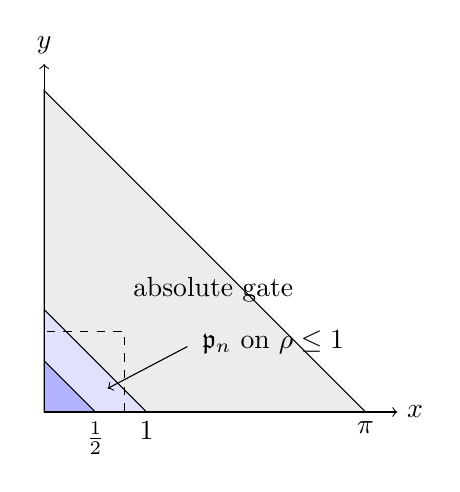
\begin{tikzpicture}[scale=1.3]
 \fill[gray!15] (0,1)--(1,0)--(3.14,0)--(0,3.14)--cycle;
 \fill[blue!12] (0,.5)--(.5,0)--(1,0)--(0,1)--cycle;
 \fill[blue!30] (0,0)--(.5,0)--(0,.5)--cycle;
 \draw (0,0)--(3.14,0)--(0,3.14)--cycle;
 \draw (.5,0)--(0,.5) (1,0)--(0,1);
 \draw[dashed] (0,0) rectangle (.7854,.7854);
 \draw[->] (0,0)--(3.45,0) node[right] {$x$};
 \draw[->] (0,0)--(0,3.4) node[above] {$y$};
 \node[below] at (.5,0) {$\frac12$};
 \node[below] at (1,0) {$1$};
 \node[below] at (3.14,0) {$\pi$};
 \node at (1.65,1.20) {absolute gate};
 \node[anchor=west] at (1.45,.68) {$\mathfrak p_n$ on $\rho\leq1$};
 \draw[->] (1.40,.64)--(.62,.23);
\end{tikzpicture}
\caption{The folded phase triangle. On the darkest triangle a
noncorner chart uses $\Delta>1/20$ together with $\mathfrak p_n$.
On $1/2\leq\rho\leq1$, $\mathfrak p_n<0$ suffices; the absolute gate covers
$\rho\geq1$. In a corner chart the dashed $\pi/4$ square has a
separate descent estimate.}
\label{fig:phase-regions}
\end{figure}

\subsection{A completed comparison model}
\label{uc:model}

Throughout the comparison argument $m=n+1$, $L=\log n$, $\bar{L}=1+L$,
$H_n=\sum_{j=1}^n j^{-1}$, and
\[
 \begin{gathered}
 x=|\alpha|,\quad y=|\beta|,\quad \rho=x+y\leq\pi,\quad
 c_e=\cos(\rho/2),\quad c_d=\cos((x-y)/2),\\
 \mathsf{a}=c_ec_d,\quad u=1-\mathsf{a},\quad z=(1-c_e)(1-c_d).
 \end{gathered}
\]
For a real number $t$, write $t_+=\max(t,0)$.
Also put $p=\sin x$, $q=\sin y$, $P=p+q$, and $d_+=(q-p)_+$.
Thus $\mathsf{a}=(\cos x+\cos y)/2\geq0$ and $2-c_e-c_d=u+z$.
Throughout, $x$ refers to the $n$-mesh and $y$ to the $m$-mesh.
A phase point is denoted $\varphi=(x,y)$.
For real $C,D$ and $0<e<\pi$, define the complete cancellation
\begin{align}\label{uc:cancellation}
 I(C,D,e)&=\int_0^\pi
 \{|C\cot t+D\cot(t+e)|-|C\cot t|-|D\cot(t+e)|\}\,dt,\notag\\
 J(v,s,e)&=I((v-s)/2,(v+s)/2,e).
\end{align}
Write $g(C,D;t)$ for this integrand, with the separation understood.
We integrate the combined integrand, whose pole limits are finite.
It is invariant under simultaneous coefficient reversal and exchange of
channels. The separation is even and $\pi$-periodic, so reduction to
$0<e\leq\pi/2$ covers every nonzero separation. At $e\equiv0$,
opposite coefficients may give a logarithmic divergence. In the row
profile below this is the integrable central logarithm at $v=\pi$.

\begin{lemma}[Cancellation and root formulas]\label{uc:cancellation-lemma}
For $v,s\geq0$, $0<e\leq\pi/2$, write
\[
 J(v,s,e)=2(s-v)_+\log\sin e+R(v,s,e).
\]
Then $R\leq0$,
\begin{align}\label{uc:R-bounds}
 |R|&\leq\max(2v,s+v)\log2,
 &|R_s|&\leq\log\frac{v+s}{|v-s|},\\
 R_e&=\frac{2\{v\cos e-\sqrt{(v^2-s^2\sin^2e)_+}\}}{\sin e}
 &&(s>v),\qquad R_e=0\quad(s\leq v).\notag
\end{align}
The derivative in $s$ is used as a locally integrable bound at $s=v$.
If
\begin{equation}\label{uc:root-Z}
 E(v,s,e)=J(v,s,e)-2s\log\sin e,\qquad
 Z(v,s,e)=2\int_e^{\pi/2}
       \frac{\sqrt{(v^2-s^2\sin^2t)_+}}{\sin t}\,dt,
\end{equation}
then $E\leq Z$, with equality for $s\geq v$.
All complete formulas extend continuously through zero coefficients
and moving equality roots.
\end{lemma}
\begin{proof}
On a sign interval the integrand is $-2$ times the smaller absolute
channel, and its primitive is a linear combination of logarithms of
sines. For $s\leq v$, with $c=(v-s)/2$, $b=(v+s)/2$, this gives
$J=2\{c\log(c/v)+b\log(b/v)\}$. For $s>v$, put
$c=(s-v)/2$, $b=(s+v)/2$. If $s\sin e\geq v$, integration gives
$J=2s\log\sin e$. Otherwise the equality roots satisfy
$\sin(2t+e)=s\sin e/v$. With
$t_1=(\arcsin(s\sin e/v)-e)/2$, the result is
\[
 J=2s\log\sin e+2\left\{
 b\log\frac{\cos t_1}{\sin(t_1+e)}
 -c\log\frac{\cos(t_1+e)}{\sin t_1}\right\}.
\]
These expressions have matching limits at every threshold, using
$0\log0=0$. Differentiation gives \eqref{uc:R-bounds}; the moving
endpoint terms cancel because the channel magnitudes agree there.
For $s>v$, $R$ increases from
$2(c\log c+v\log v-b\log b)$ at $e=0$ to zero at $e=\pi/2$.
These endpoints, and the entropy formula $2\{c\log(c/v)+b\log(b/v)\}$ for $s\leq v$, give its
sign and size bounds. Subtracting $2s\log\sin e$ gives derivative
$-2\sqrt{(v^2-s^2\sin^2e)_+}/\sin e$ in the root regime and zero
beyond its threshold. Integration from that threshold proves $E=Z$
for $s\geq v$. For $s<v$, $J\leq0$ and
$\sqrt{v^2-s^2\sin^2t}\geq s\cos t$, whence
$Z\geq-2s\log\sin e\geq E$. The case $v=0$ is direct.
\end{proof}

\paragraph{Elementary constants.}
Write $\zeta(s)=\sum_{k\geq1}k^{-s}$ for $s>1$.
The following rational brackets are used throughout the comparison proof;
we state their construction before their first use. For logarithms, with a positive integer $J_{\log}$ and
$w_{\log}=(z_{\log}-1)/(z_{\log}+1)$ and $z_{\log}>1$,
\begin{equation}\label{ul:log-series}
 0\leq\log z_{\log}-2\sum_{j=0}^{J_{\log}-1}\frac{w_{\log}^{2j+1}}{2j+1}
 \leq\frac{2w_{\log}^{2J_{\log}+1}}{(2J_{\log}+1)(1-w_{\log}^2)}.
\end{equation}
Reduce $z_{\log}$ to $[1,2]$ by powers of two and use $J_{\log}=48$. Write
$\mathcal A_N(q)=\sum_{r=0}^{N-1}(-1)^r/((2r+1)q^{2r+1})$ and
$\zeta_{10}(s)=\sum_{k=1}^{10}k^{-s}$. The alternating arctangent series gives
$\mathcal A_{40}(q)<\arctan(1/q)<\mathcal A_{39}(q)$ for $q>1$.
Machin's identity is $\pi=16\arctan(1/5)-4\arctan(1/239)$.
Together with convexity these give the rational constructions
\[
 \begin{gathered}
 16\mathcal A_{40}(5)-4\mathcal A_{39}(239)<\pi
                <16\mathcal A_{39}(5)-4\mathcal A_{40}(239),\\
 \zeta_{10}(s)+\frac1{(s-1)10^{s-1}}-\frac1{2\cdot10^s}
 \leq\zeta(s)\leq \zeta_{10}(s)+\frac{2^{s-1}}{(s-1)21^{s-1}},\\
 H_{256}-\log257<\gamma<H_{256}-\log(513/2).
 \end{gathered}
\]
The zeta bounds are the trapezoid and midpoint comparisons for $t^{-s}$;
the gamma bounds follow from the monotone sequences $H_M-\log(M+1)$
and $H_M-\log(M+1/2)$.
In particular the consumed elementary bounds are
\[
\begin{gathered}
23/40<\gamma<3/5,\qquad197/20<\pi^2<10,\qquad3<\pi<22/7,\\
69/100<\log2<6932/10000,\qquad11/10<\log\pi<23/20,\\
\log(\pi/2)<23/50,\qquad161/100<\mathfrak k_0<9/5,
\quad\mathfrak k_0=2\gamma+4\log2-2\log\pi.
\end{gathered}
\]
For the gamma brackets, the increments of $H_M-\log(M+1)$ are
positive because $\log(1+t)<t$; those of
$H_M-\log(M+1/2)$ are negative because
$\log((1+t)/(1-t))>2t$, with $t=1/(2M+2)$.
Alternating Taylor sums enclose sine and cosine whenever their omitted
terms decrease in modulus; the error has the sign and at most the
modulus of the first omitted term.
These finite rational comparisons, the $K=3$ kappa series below and the
scalar-gate base values are evaluated by
\texttt{code/onset512\_analytic/check.py}, using Python integers and
\texttt{Fraction}; the repository contains its executed receipt at
\path{code/onset512_analytic/receipt.json}.

The scalar reciprocal pair and its continuous periodic profile are
\begin{align}\label{uc:scalar-definitions}
 \mathcal C(t)&=2\gamma+\frac1t+\frac1{1-t}
 +\sum_{k\geq1}\left\{\frac1{k+t}+\frac1{k+1-t}-\frac2k\right\},
 \notag\\
 C_0&=\mathcal C(1/2)=2\gamma+4\log2,\notag\\
 \Phi(t)&=\frac{\sin\pi t}{\pi}\{\mathcal C(t)-2\log\pi\},
 \quad\Phi(0)=\Phi(1)=1,\notag\\
 f(w)=\Phi(1/2+w/(2\pi)).
\end{align}
Extend $\Phi$ with period one. Then $f$ is even with period $2\pi$.
We use $\psi(t)=-\gamma+\sum_{k\geq0}\{(k+1)^{-1}-(k+t)^{-1}\}$,
so $\mathcal C(t)=-\psi(t)-\psi(1-t)$.

We write $\zeta(s)=\sum_{k\geq1}k^{-s}$ for $s>1$.
The Lipschitz constant $\operatorname{Lip}(f)$ is the least $K$ such
that $|f(w)-f(v)|\leq K|w-v|$.
For a periodic function $h$, $\operatorname{Var}_{\rm per}h$ is the
supremum of the sums of absolute changes along partitions of one
period, counting the joined endpoint once. Such a function is of
bounded variation (BV) when this supremum is finite. Its derivative
measure $dh$ records its changes, including jumps; its
total-variation measure $|dh|$ records their absolute sizes.
In particular $df'$ below includes both the ordinary second derivative
and the cusp jump. The unit point mass $\delta_\pi$ satisfies
$\int\varphi\,d\delta_\pi=\varphi(\pi)$ for periodic continuous
$\varphi$. An inequality $\nu\leq c\,dw$ between measures means
$\int\varphi\,d\nu\leq c\int\varphi\,dw$ for every nonnegative
continuous periodic $\varphi$.
The finite part below means the cutoff limit after its
displayed logarithmic counterterm is added.

\begin{lemma}[The scalar maximum, including its cusp]\label{uc:scalar-maximum}
The function $f$ is Lipschitz, $f'$ has bounded variation on the circle,
and, for its ordinary second derivative $f''$ on $(-\pi,\pi)$,
\begin{equation}\label{uc:scalar-bounds}
 \begin{gathered}
 \frac12<f\leq1,\quad \operatorname{Lip}(f)<2,\quad
 |f''|<1,\quad |f'''|<13/20,\quad
 \operatorname{Var}_{\rm per}f'<4,\\
 df'=f''(w)\,dw-J_0\delta_\pi\leq\frac3{\pi^2}\,dw,
 \quad J_0=\frac{2(\log\pi-\gamma)}\pi>\frac1\pi.
 \end{gathered}
\end{equation}
The endpoint atom is counted once. The finite part
\begin{equation}\label{uc:H}
 H(w)=\frac1\pi\lim_{\epsilon\downarrow0}
 \left\{\int_\epsilon^{2\pi-\epsilon}
 \frac{f(w+t)}{2\sin(t/2)}\,dt+2f(w)\log\frac\epsilon\pi\right\}
\end{equation}
satisfies $H(w)\leq H_0:=H(0)$ for all real $w$.
\end{lemma}
\begin{proof}
On $0<t\leq1/2$ the defining series becomes
\[
 \mathcal C(t)=t^{-1}+2\gamma+Q(t),\qquad
 Q(t)=2\sum_{j\geq1}\zeta(2j+1)t^{2j}.
\]
Integral comparison gives $\zeta(3)<5/4$, hence
$Q\leq4t^2$, $Q'\leq5t/(1-t^2)^2\leq(32/3)t$, and
$Q''\leq Q''(1/2)=28\zeta(3)-16<19$
(the weaker absolute bound $608/27$ is also convenient).
With $\mathfrak{k}=2\gamma-2\log\pi$,
\[
 \Phi(t)=\frac{\sin\pi t}{\pi t}
             +\mathfrak{k}\frac{\sin\pi t}\pi+Q(t)\frac{\sin\pi t}\pi.
\]
The elementary bounds $\log\pi>11/10$ and $\gamma<3/5$,
together with $Q\leq1$, give $\mathfrak{k}+Q<0$. Hence this is at most one. For the lower bound, put
$\mathfrak{k}_0=C_0-2\log\pi$ and $c_s=\cos(\pi s/2)$. Reciprocal pairing gives
\begin{equation}\label{uc:f-series}
 f(w)=\frac{\cos(w/2)}\pi
 \left\{\mathfrak{k}_0+4w^2\sum_{\ell\geq1,\ \ell\ {\rm odd}}
       \frac1{\ell(\ell^2\pi^2-w^2)}\right\},\quad |w|<\pi.
\end{equation}
The inequality $c_s\geq(3/4)(1-s^2)$ follows by differentiating
$\sin(\pi r/2)-(3/4)r(2-r)$, $r=1-s$: its second derivative
changes sign once, and its first derivative ends at zero. Keeping
$\ell=1$ in \eqref{uc:f-series}, and using
$1-c_s\leq\pi^2s^2/8$, $\mathfrak{k}_0<2$, $\pi^2<10$, gives
$\pi f(\pi s)\geq c_s\mathfrak{k}_0+4c_ss^2/(1-s^2)\geq \mathfrak{k}_0$.
The elementary bounds $\gamma>23/40$, $\log2>69/100$,
$\log\pi<23/20$ give $\mathfrak{k}_0>161/100>\pi/2$.

Differentiating the three terms of $\Phi$ bounds their first
 derivatives by $2,5,4$, respectively. Their five second-derivative
contributions have absolute bounds
$10/3,10,608/81,32/3,10/3$, whose sum is less than $35$.
Thus $\operatorname{Lip}(f)<6/\pi<2$ and $|f''|<35/(4\pi^2)<1$.
For the one-sided bound use
\[
 \left(\frac{\sin\pi t}{\pi t}\right)''
 \leq-\pi^2(1/3-\pi^2/40)\leq-\pi^2/12,
 \quad \frac{t(1/2-t)}{(1-t^2)^2}\leq\frac3{40}.
\]
For the latter, $3+34t^2+3t^4-20t
=34(t-5/17)^2+1/17+3t^4>0$.
Since $-\mathfrak{k}<5/4$, differentiation gives
$\Phi''\leq-\pi^2/12+2\pi+19/\pi<12$.
At an integer $\Phi'$ has jump $2\mathfrak{k}<0$; reflection matches its
ordinary derivative at the half integer. Scaling proves the measure
bound in \eqref{uc:scalar-bounds}, including the stated atom.
The positive mass of $df'$ is at most $6/\pi$, its total mass is
zero, and therefore its variation is at most $12/\pi<4$.

For the remaining derivative facts an endpoint-cancelled formula is
useful:
\begin{equation}\label{uc:f-integral}
 f(w)=f(0)\cos(w/2)+2\int_0^{1/2}
       \frac{\cos(wt)-\cos(w/2)}{\cos\pi t}\,dt,\qquad |w|\leq\pi.
\end{equation}
To derive it, integrate the numerator against $\cos((2j+1)\pi t)$;
the result is
$(-1)^j\cos(w/2)w^2/[(2j+1)\pi((2j+1)^2\pi^2-w^2)]$.
For $0<r<1$, insert the convergence factors $r^{2j+1}$ in the
kernel sum (Abel regularization):
\[
 \begin{aligned}
 &\sum_{j\geq0}(-1)^jr^{2j+1}\cos((2j+1)\pi t)\\
 &\quad=\frac{r(1+r^2)\cos\pi t}{(1-r^2)^2+4r^2\cos^2\pi t}\\
 &\quad\longrightarrow\frac1{2\cos\pi t}.
 \end{aligned}
\]
For $r\geq1/2$ it is bounded by $5/(8\cos\pi t)$, while the
numerator is $O(1/2-t)$ and $\cos\pi t\geq2(1/2-t)$.
The dominated-convergence theorem permits passage of a pointwise
limit through an integral when the integrands have a common integrable
absolute bound. Here the displayed kernel bound and the vanishing
numerator supply that bound. The same mean-value estimate applies to
the first three differentiated numerators, uniformly for $|w|\leq\pi$,
since their $t$ derivatives are bounded on this compact rectangle.
Thus it proves \eqref{uc:f-integral}, including its endpoints, and
permits three derivatives. In particular
\[
 f'''(w)=\frac{f(0)}8\sin(w/2)
 +2\int_0^{1/2}\frac{t^3\sin(tw)-\sin(w/2)/8}{\cos\pi t}\,dt.
\]
The numerator's $t$ derivative has magnitude at most
$3/4+\pi/8<23/20$, giving $|f'''|<23/40+3/40=13/20$.
For $0<w\leq\pi$, monotonicity of $r\cot r$ gives
$\sin(tw)/\sin(w/2)\leq\sin\pi t$. Here $f(0)=\mathfrak k_0/\pi<(9/5)/3=3/5$, so $f(0)/8<3/40$. Split
$[0,1/2]$ at $1/4,3/8$, use respectively $\sin\pi t\leq(22/7)t$
and $t^3\sin\pi t\leq27/512$, and discard the negative last part.
This yields
\[
 \frac{f'''(w)}{\sin(w/2)}
 <\frac3{40}+\frac{44}{35\cdot1024}-\frac1{16}-\frac{37}{2048}
 =-\frac{311}{71680}<0.
\]
Consequently $f''$ is even and decreases radially.

Pairing endpoints in \eqref{uc:H} gives the absolutely convergent
formula
\[
 H(w)=\lambda_0f(w)+\frac1\pi\int_0^\pi
 \frac{f(w+t)+f(w-t)-2f(w)}{2\sin(t/2)}\,dt,
 \qquad \lambda_0=\frac2\pi\log\frac4\pi<\frac1{2\pi}.
\]
The bound follows from $\pi>25/8$ and $\mathrm e^{1/4}>32/25$.
Set $\mathcal{W}(t)=\int_{|t|}^\pi\log\cot(s/4)\,ds$ on the circle.
It is bounded, nonnegative and radially decreasing. Integrating the
identity
$f(w+t)+f(w-t)-2f(w)=\int_{-t}^t(t-|r|)\,df'(w+r)$
(valid for $f'$ of bounded variation) against
$df'$ gives
\[
 H(w)=\lambda_0f(w)+\frac1\pi\int_{-\pi}^{\pi}\mathcal{W}(t)f''(w+t)\,dt
                  -\frac{J_0}\pi \mathcal{W}(\pi-|w|),\quad |w|\leq\pi.
\]
Fubini's theorem allows the order of integration to be exchanged when
the absolute integral is finite. Here the integrated triangular weight
is the bounded function $\mathcal W$, so the absolute integral against
$|df'|$ is at most $\|\mathcal W\|_\infty\operatorname{Var}_{\rm per}f'<\infty$.
The value $\mathcal W(\pi)=0$ counts the atom only once. Subtract the
minimum of $f''$ to make it nonnegative. The layer-cake identity
$h(t)=\int_0^\infty\mathbf1_{\{h(t)>r\}}\,dr$ for $h\geq0$
reduces its convolution with $\mathcal{W}$ to lengths
of intersections of two centered circular arcs; a translate cannot
increase such a length. The convolution is therefore largest at zero.
The measure bound implies $f(w)-f(0)\leq3w^2/(2\pi^2)$, and
$\mathcal{W}(\pi-|w|)\geq w^2/4$, since the derivative of
$\log\cot((\pi-s)/4)$ is $1/(2\cos(s/2))\geq1/2$.
Thus $H(w)-H_0\leq-(\pi-3)w^2/(4\pi^3)\leq0$.
Continuity and periodicity include the closed endpoints.
\end{proof}

For $0<v<2\pi$ define the row coefficients and profile
\begin{align}\label{uc:row-profile}
 C_-(v)&=(p-q-2\mathsf{a}\cot(v/2))/4,\quad C_+(v)=(p+q+2\mathsf{a}\cot(v/2))/4,\notag\\
 \eta_-(v)&=\tfrac12+(x-y+v)/(2\pi),\quad
 \eta_+(v)=\tfrac12+(x+y-v)/(2\pi),\notag\\
 A(v)&=2(|C_-(v)|+|C_+(v)|)/\pi,\notag\\
 \mathcal B(v)&=\frac{c_e\Phi(\eta_-(v))+c_d\Phi(\eta_+(v))}
                         {2\sin(v/2)}+\frac{I(C_-(v),C_+(v),v)}\pi.
\end{align}
Write $\mathcal{V}(L,v)=A(v)L+\mathcal B(v)$ and
$U_0=c_ef(x-y)+c_df(x+y)$, $B_0=4\mathsf{a}/\pi^2$,
$D_0=U_0/\pi+B_0\log\pi$. The completed model is
\begin{equation}\label{uc:completed-model}
 \begin{gathered}
 M_\infty(x,y,L)=\frac{4\mathsf{a}}{\pi^2}L^2+b_{\rm full}L+C_\infty,\\
 b_{\rm full}=\frac{2U_0}\pi+
 \frac{8\mathsf{a}\log2+4\mathsf{a}\log \mathsf{a}+2(xp+yq)}{\pi^2},\\
 E_\infty=\frac {\mathsf{a}}{3}+
 \frac{\mathsf{a}}{\pi^2}\mathcal C(1/2+(x-y)/(2\pi))
                         \mathcal C(1/2+(x+y)/(2\pi)),\\
 C_\infty=E_\infty+\lim_{\epsilon\downarrow0}
 \left\{B_0\log^2\frac\epsilon\pi+2D_0\log\frac\epsilon\pi
            +\frac1\pi\int_\epsilon^{2\pi-\epsilon}\mathcal B(v)\,dv\right\}.
 \end{gathered}
\end{equation}
Weighted endpoint products and $\mathsf{a}\log \mathsf{a}$ have their continuous values.
The model is the completed integral of the row profile
$\mathcal V(L,v)=A(v)L+\mathcal B(v)$: the finite sum averages the
same profile over the row mesh. Cutting its integral at one mesh step
$\epsilon=\pi/n$ turns $\log(\epsilon/\pi)$ into $-L$; its
counterterms supply the quadratic and linear logarithms above.
The term $E_\infty$ completes the endpoint rows, as proved in
\eqref{uc:reference-match}.

The limit exists uniformly on the closed phase triangle. We give an
explicit envelope, also needed for the finite mesh. For either folded
side $v_L(t)=t$, $v_R(t)=2\pi-t$, $0<t\leq\pi/4$,
\begin{equation}\label{uc:endpoint-envelope}
 \left|\mathcal B(v_s(t))-
       \frac{U_0+(4\mathsf{a}/\pi)\log t}{t}\right|
 \leq7+\frac P\pi\left(3+2\log\frac{4\pi}{t}\right).
\end{equation}
For $\delta=x-y$, define the pole numerators
\[
 N_L(t)=c_ef(t+\delta)+c_df(t-\rho),\qquad
 N_R(t)=c_ef(t-\delta)+c_df(t+\rho).
\]
Both have value $U_0$ at zero. To prove the envelope, compare
$I(C,D,t)$ with $I(-w,w,t)$, where
$w=\mathsf{a}\cot(t/2)/2$ and each coefficient displacement is at most $P/4$.
For general displacements at most $\varepsilon_d$, remove pole arcs of
radius $t/8$. If $w\geq4\varepsilon_d$, the own channel dominates there
and the two cancellations differ by at most $8\varepsilon_d/7$ in
integral. If $w<4\varepsilon_d$, both complete cancellations are bounded
by twice the other channel, costing at most $72\varepsilon_d/7$.
On the complement their difference is at most
$2\varepsilon_d(|\cot z|+|\cot(z+t)|)$, whose integral is at most
$8\varepsilon_d\log(4\pi/t)$. Thus
\[
 |I(C,D,t)-I(-w,w,t)|\leq\varepsilon_d[11+8\log(4\pi/t)],
 \qquad I(-w,w,t)=4w\log\sin t.
\]
For the pole numerator $N_s$, $|N_s(t)-U_0|\leq12t/\pi$,
and $|N_s|\leq c_e+c_d\leq2\leq8$ by $|f|\leq1$. The chord bound $\sin t\geq2t/\pi$ on $[0,\pi/2]$ gives a pole remainder at most
$6+\pi t/6$. Finally
$|2\mathsf{a}\cot(t/2)\log\sin t-(4\mathsf{a}/t)\log t|
\leq \mathsf{a}t(1+|\log t|)$. To see the regular pole term explicitly, write
\[
 \frac{N_s(t)}{2\sin(t/2)}-\frac{U_0}{t}
 =\frac{N_s(t)-U_0}{t}
  +N_s(t)\left\{\frac1{2\sin(t/2)}-\frac1t\right\}.
\]
The chord inequality and $0\leq t-2\sin(t/2)\leq t^3/24$ give
$0\leq[2\sin(t/2)]^{-1}-t^{-1}\leq\pi t/48$.
Thus the displayed pole term has absolute value at most $6+\pi t/6$.
For $0<t\leq\pi/4<1$, the remaining reference error is at most
$t(1+|\log t|)/\pi\leq1/\pi$, so its constant contribution is
\[
 6+\frac{\pi^2}{24}+\frac1\pi<7.
\]
The displacement contribution satisfies
$(P/(4\pi))[11+8\log(4\pi/t)]\leq(P/\pi)[3+2\log(4\pi/t)]$.
Together these prove \eqref{uc:endpoint-envelope}.
Its integrable right side makes the finite parts uniformly Cauchy.
Lemma~\ref{uc:cancellation-lemma} bounds all central root transitions by an
integrable multiple of $1+|\log\sin t|$; hence their limits are
continuous in phase, including the axes and vertices.

The logarithmic coefficient is obtained by integrating the row coefficient.
Put $X=\max(x,y)$, $Y=\min(x,y)$ and $T_t=2\mathsf{a}\cot(t/2)$. Then
$\pi(A(t)+A(2\pi-t))$ is respectively
$2T_t$, $T_t+p+q$, $2\sin X$ on the intervals cut by
$\pi-X-Y$ and $\pi-X+Y$. Integrating with
$\int T_t\,dt=4\mathsf{a}\log\sin(t/2)$ gives
\[
 \int_0^\pi\{A(t)+A(2\pi-t)-8\mathsf{a}/(\pi t)\}\,dt
 =\{8\mathsf{a}\log(2/\pi)+4\mathsf{a}\log \mathsf{a}+2(xp+yq)\}/\pi.
\]
The row average contributes the additional endpoint coefficient $2D_0$:
\[
 b_{\rm full}=2D_0+\frac1\pi\int_0^\pi
       \{A(t)+A(2\pi-t)-8\mathsf a/(\pi t)\}dt.
\]
Since $2D_0=2U_0/\pi+8\mathsf a\log\pi/\pi^2$, this gives exactly
the coefficient in \eqref{uc:completed-model}.
The max formulas give
$|\pi A(t)-T_t|\leq1$ and $|\pi A(2\pi-t)-T_t|\leq1$.
Also $T_t-4\mathsf a/t=2\mathsf a\{\cot(t/2)-2/t\}$ is uniformly
bounded on $(0,\pi]$. These bounds dominate the subtracted integrand
independently of phase, so dominated convergence includes $\mathsf{a}=0$.

\begin{lemma}[Correlated model bounds]\label{uc:master}
Put
\[
 \begin{gathered}
 b_*=C_0-7/2,\quad B=C_0^2/\pi^2,\quad d_*=C_0b_*/\pi^2,
 \quad v_*=7b_*/(2\pi^2),\\
 g_0=4(\log^2\pi-\log^22)/\pi^2,\quad
 \mathfrak{j}=H_0+d_*-g_0,\quad t_0=2\log2/\pi.
 \end{gathered}
\]
With $C_*=C_\infty(0,0)$ and $b_c=8(\gamma+\log(8/\pi))/\pi^2$,
\begin{align}\label{uc:model-loss}
 b_{\rm full}-b_c&\leq3u/\pi^2,& b_{\rm full}&<79/(5\pi^2),\notag\\
 C_\infty-C_*&\leq-\mathfrak{j}u+t_0p-(H_0+v_*)z\leq-\mathfrak{j}u+t_0p,
 &C_\infty&<9/4.
\end{align}
On $\rho\leq\pi/2$ there is the exact decomposition
\begin{equation}\label{uc:central-decomposition}
 C_\infty=E_\infty+c_eH(x-y)+c_dH(x+y)-(1/3+g_0)\mathsf{a}+E_c,
\end{equation}
where
\begin{equation}\label{uc:Ec}
 \begin{aligned}
 E_c=\frac1{\pi^2}\int_0^{\pi/2}
 \bigl\{&J(p/2,\mathsf{a}\tan(t/2)+q/2,t)\\
 &+J(p/2,|\mathsf{a}\tan(t/2)-q/2|,t)-4\mathsf{a}\tan(t/2)\log\sin t\bigr\}\,dt.
 \end{aligned}
\end{equation}
Consequently
\begin{equation}\label{uc:regular-loss}
 (C_\infty-E_c)-C_*\leq-\mathfrak{j}u-(H_0+v_*)z\leq0.
\end{equation}
\end{lemma}
\begin{proof}
First the reciprocal-pair series implies, for $|\theta|\leq\pi$,
\begin{equation}\label{uc:weighted-C}
 \cos(\theta/2)\mathcal C(1/2+\theta/(2\pi))
       \leq C_0-b_*\{1-\cos(\theta/2)\}.
\end{equation}
Here is a direct verification with its endpoint normalization.
For $0<s<1$, $c=\cos(\pi s/2)$, the tangent partial fraction
$\frac\pi2\tan(\pi s/2)=\sum_{\ell\geq1,\ \ell\ {\rm odd}}
2s/(\ell^2-s^2)$ gives
\[
 \frac{d}{ds}\log\frac{1-s^2}{c}
 =\sum_{\ell\geq3,\ \ell\ {\rm odd}}\frac{2s}{\ell^2-s^2}
 \geq2s(\pi^2/8-1).
\]
Integration yields $cs^2/[(1-c)(1-s^2)]\leq8/\pi^2$.
Also $\sum_{\ell\geq3,\ \ell\ {\rm odd}}1/[\ell(\ell^2-1)]
=3/4-\log2$, by partial fractions. Therefore
\[
 \frac{c\{\mathcal C(1/2+s/2)-C_0\}}{1-c}
 \leq\frac{32}{\pi^2}(7/4-\log2)<7/2.
\]
The endpoint weighted increment tends to $\pi<7/2$; symmetry and
continuity prove \eqref{uc:weighted-C} on the closed interval.
Multiplication of its positive factors gives
\begin{equation}\label{uc:endpoint-loss}
 E_\infty\leq \mathsf{a}/3+B-d_*u-v_*z.
\end{equation}
If $D_{\mathcal C}=\mathcal C(1/2+(x+y)/(2\pi))+
\mathcal C(1/2+(x-y)/(2\pi))-2C_0$, then $\mathsf{a}D_{\mathcal C}\leq(7/2)u$.
Substitution in $b_{\rm full}$ gives exactly
\[
 b_{\rm full}-b_c=\frac2{\pi^2}
 \{\mathsf{a}D_{\mathcal C}+2\mathsf{a}\log \mathsf{a}+xp+yq-4(\gamma+\log(8/\pi))u\}.
\]
Use $xp+yq\leq4u$, $\mathsf{a}\log \mathsf{a}\leq0$, and
$3/2<\gamma+\log(8/\pi)<8/5$. For the lower bound the first two
terms of $2\operatorname{atanh}(17/39)$ give
$\log(28/11)>37/40$; the remaining constants follow from
$23/40<\gamma<3/5$, $3<\pi<22/7$. This proves both coefficient bounds.

Split the completed finite part into its scalar pole term
$c_eH(x-y)+c_dH(x+y)$ and cancellation term. The cancellation
parameters at $0<t<\pi$ are
$J(p/2,(q+T_t)/2,e_t)$ and
$J(p/2,|q-T_t|/2,e_t)$, $e_t=\min(t,\pi-t)$.
Since $R\leq0$, their sum is at most
\[
 4\mathsf{a}\cot(t/2)\log\sin t+2p|\log\sin t|.
\]
Indeed their logarithmic coefficient is
$(q+T_t-p)_++(|q-T_t|-p)_+\geq2T_t-2p$.
Define $\operatorname{Li}_2(z)=\sum_{k\geq1}z^k/k^2$ on $[0,1]$;
its derivative is $-\log(1-z)/z$ on $(0,1)$.
The integral of $|\log\sin t|$ is $\pi\log2$. A primitive of the
first term is
$4\mathsf{a}\log^2(2\sin(t/2))-4\mathsf{a}\log^22-2\mathsf{a}\operatorname{Li}_2(\sin^2(t/2))$.
Since $\operatorname{Li}_2(1)=\sum k^{-2}=\pi^2/6$, its endpoint
counterterm leaves $-(1/3+g_0)\mathsf{a}$.
On $\rho\leq\pi/2$, $2\mathsf{a}\geq p+q$, and the endpoint half is
root-free: $(2\mathsf{a}\cot(t/2)-q)\sin t\geq2\mathsf{a}-q\geq p$ for
$0<t\leq\pi/2$. Reflecting the central half gives exactly
\eqref{uc:central-decomposition}. Lemma~\ref{uc:cancellation-lemma} bounds its
integrand by $10|\log\sin t|+4\log2$, including equality at the
closed boundary. Dominated convergence justifies all boundary limits.
Apply Lemma~\ref{uc:scalar-maximum} and \eqref{uc:endpoint-loss}, then use
$2-c_e-c_d=u+z$. At zero this gives
$C_*=B-g_0+2H_0$ and proves both correlated losses.

The corner expansion identifies the same constant as
$C_*=4(\gamma+\log(8/\pi))^2/\pi^2+\kappa$:
at zero $S_n=\Lambda_c(n)$ and the finite error proved below tends
to zero. That absolute finite-error proof uses no model-loss constants,
so this identification does not create a circular dependency. Hence
\begin{equation}\label{uc:origin-identity}
 H_0=\kappa/2+(2\mathfrak{k}_0/\pi^2)\log(2/\pi).
\end{equation}
The needed constant inequalities have an elementary finite reduction:
\begin{equation}\label{uc:coarse-input}
 \kappa>9/10,\qquad C_*<4629/2500.
\end{equation}
Define
\begin{align*}
 \mathfrak a_i&=1-2\sum_{r=1}^i\frac{\zeta(2r)}{4^r}\quad(i\geq0),
 \qquad\mathfrak b_0=7\zeta(3)/8,\\
 \mathfrak b_\ell&=(1-2^{-2\ell-3})\zeta(2\ell+3)
              -(1-2^{-2\ell-1})\zeta(2\ell+1)\quad(\ell\geq1),\\
 c_k&=\sum_{i+\ell=k}\mathfrak a_i\mathfrak b_\ell.
\end{align*}
Cancelling the endpoint pole before multiplication gives
\begin{equation}\label{uc:kappa-series}
 \begin{gathered}
 \frac{t^2\cot(\pi t/2)}{1-t^2}
       =\frac{2t}\pi\sum_{i\geq0}\mathfrak a_it^{2i},\qquad
 (1-t^2)\sum_{r\geq1,\ r\text{ odd}}
       \frac1{r(r^2-t^2)}=\sum_{\ell\geq0}\mathfrak b_\ell t^{2\ell},\\
 \kappa=\frac8{\pi^2}\sum_{k\geq0}\frac{c_k}{k+1},\qquad
 \left|\kappa-\frac8{\pi^2}\sum_{k=0}^K\frac{c_k}{k+1}\right|
       \leq\frac8{3(K+2)4^{K+1}}.
 \end{gathered}
\end{equation}
The cotangent partial fraction gives
$\mathfrak a_i=2\sum_{r\geq1}(4r^2)^{-i}/(4r^2-1)\leq4^{-i}$;
reciprocal expansion gives the second series, with $\mathfrak b_0<10/9$
and $|\mathfrak b_\ell|<9^{-(\ell-1)}(1/27+\int_3^\infty s^{-3}ds)<9^{-\ell}$
for $\ell\geq1$. Hence $|c_k|<2\cdot4^{-k}$: uniform convergence
permits integration, and the geometric majorant with $8/\pi^2<1$
gives the tail.

Use $K=3$, whose tail is $1/480$. Substituting the elementary brackets above into the $K=3$ sum in
\eqref{uc:kappa-series}, and adding its tail, gives
\[
917166/10^6<\kappa<921489/10^6,\qquad
C_*<1847940/10^6<4629/2500.
\]
All endpoints follow by finite rational comparisons. In particular,
\begin{equation}\label{uc:scalar-constants}
 \begin{gathered}
 H_0>7/25,\qquad d_*>39/250,\qquad g_0<43/125,\\
 \mathfrak j>23/250,\qquad 0<t_0<221/500.
 \end{gathered}
\end{equation}
For example $H_0>9/20-828/4925>7/25$;
$C_0>39/10$, $b_*>2/5$ give $d_*>39/250$;
and $g_0<(80/197)((23/20)^2-(69/100)^2)<43/125$.
Thus $\mathfrak j>7/25+39/250-43/125=23/250$.
Finally $u\geq(1-\cos x)/2$ gives
$C_\infty\leq C_*-\mathfrak j/2+(\mathfrak j/2)\cos x+t_0\sin x$.
Cauchy--Schwarz bounds the last two terms by
$\sqrt{\mathfrak j^2/4+t_0^2}$, since $\cos^2x+\sin^2x=1$.
For $\delta=9/4-C_*>249/625$,
\[
 \delta^2+\delta\mathfrak j-t_0^2>
 (249/625)^2+(249/625)(23/250)-(221/500)^2
 =71/6250000>0.
\]
Squaring the positive quantities $\delta+\mathfrak j/2$ and
$\sqrt{\mathfrak j^2/4+t_0^2}$ proves $C_\infty<9/4$.
\end{proof}

\begin{lemma}[The paired central roots]\label{uc:central-pair}
On $x,y\geq0$, $\rho\leq\pi/2$, put
\[
 b=2\arctan(q/(2\mathsf a)),\qquad
 B_\beta=\frac4{\pi^2}\int_0^b
       (q/2-\mathsf a\tan(t/2))[-\log\sin t]dt.
\]
Then $0\leq b\leq\rho$, $B_\beta\geq0$, $E_c(0,y)=-B_\beta$, and
\begin{equation}\label{uc:central-pair-general}
 E_c\leq\frac{4I_4}{\pi^2}\frac{p^{3/2}}{\sqrt{\mathsf a}}-B_\beta,
 \qquad I_4=\int_0^1\sqrt{1-t^4}dt<319/360.
\end{equation}
In particular,
\begin{equation}\label{uc:central-pair-bounds}
 E_c\leq5x^{3/2}/12-B_\beta\qquad(\rho\leq1).
\end{equation}
\end{lemma}
\begin{proof}
The phase identity $(\cos x+\cos y)\tan(\rho/2)=p+q$ gives
$b\leq\rho$. Using \eqref{uc:root-Z}, the exact integrand rearranges
as two $E$ terms minus $B_\beta$. Put $v=p/2$, $\delta=q/2$.
Tonelli's theorem permits the order of integration to be exchanged
for a nonnegative measurable integrand, even before finiteness has
been proved. The $Z$ integrands are nonnegative, so it applies here;
the substitution $w=\mathsf{a}\tan(e/2)$ gives for their sum
\[
 2\int_0^{\pi/2}\frac1{\sin t}\int_{\mathbb R}
 \frac{2\mathsf{a}\,\mathbf1_{|w|\leq\mathsf a\tan(t/2)}}{\mathsf{a}^2+w^2}
        \sqrt{(v^2-(w-\delta)^2\sin^2t)_+}\,dw\,dt.
\]
Both inner factors are even and radially decreasing. Layer cake for
interval intersections shows that translation by $\delta$ cannot
increase the integral. It is therefore at most
$2F(v,\mathsf{a})$, where $F(v,\mathsf{a})=\int_0^{\pi/2}Z(v,\mathsf{a}\tan(e/2),e)\,de$.
For $\tau=v/\mathsf{a}\leq1$, a second Tonelli interchange, preserving
$e<t$, gives
\[
 F=4v\tau\int_0^1\sqrt{1-r^2}\,K(\tau r)\,dr,
 \quad K(k)=\int_{\arccos(1-k)}^{\pi/2}\frac{dt}{\sin^2t+k^2}
 \leq\frac1{\sqrt{2k}}.
\]
Indeed $w=\cot t$ bounds $K(k)$ by
$(1-k)/\sqrt{k(2-k)}\leq1/\sqrt{2k}$, using
$2(1-k)^2\leq2-k$. Thus
$F\leq4\sqrt2 I_4v^{3/2}/\sqrt {\mathsf{a}}$,
$I_4=\int_0^1\sqrt{1-r^4}\,dr<319/360$; the latter follows by
squaring $1-u/2-u^2/8\geq\sqrt{1-u}$ and integrating $u=r^4$.
The resulting bound for $E_c+B_\beta$ is
$4I_4p^{3/2}/(\pi^2\sqrt {\mathsf{a}})$.
For $\rho\leq1$, $\mathsf a\geq49/64$. Together with
$\pi^2>197/20$ and $p\leq x$, this gives $5/12$.
The inequality $2\mathsf a\geq p+q$ on $\rho\leq\pi/2$ ensures
$v/\mathsf a\leq1$ in the preceding substitution. Finiteness follows
also from $Z\leq2v\log(2/e)$, and at $v=0$ the two $E$ terms
vanish. This proves the boundary identity $E_c(0,y)=-B_\beta$.
\end{proof}

\subsection{Finite-degree comparison with the model}
\label{uc:finite-comparison}

Hereafter $n\geq32$. Put
$D_\phi=\mathsf a[((52/\pi^2)\bar L+7)/n+20\bar L/(\pi n^2)]+10/n^2$
for the phase-dependent row allowance. An allowance is an explicit upper bound on a named error. All allowances are explicit scalar functions of
real $n$; the interpolation degree remains integral. Define once
\begin{align}\label{uc:constants}
 \mathfrak{T}&=(4L^2-3L)/\pi^2,\quad b_0=4/\pi^2,\quad r_0=\log(5/2)+1/18,\notag\\
 D&=\frac{(52/\pi^2)\bar L+7}{n}+\frac{10}{n^2}+\frac{20\bar L}{\pi n^2},\notag\\
 \mathcal M&=\frac{b_0(2L+2r_0)}n
 +\frac{4+b_0(L+1/n)}{4n^2-1}+\frac{b_0}{(2n-1)^2}\notag\\
 &\qquad+\frac{5+b_0(\log(n+1/2)+2)}{4(n-1/2)^2},\notag\\
 \bar e&=D+\mathcal M+1/n,\qquad
 K_D=\frac{[6+16/(3\pi)]\bar L+2/\pi}{n},\notag\\
 A_4&=4/n+40\bar L/(\pi n^2),\quad C_4=A_4+20/n^2,
 \quad d_\beta=(17L+27)/n^2,\notag\\
 J_W&=((3/2)\bar L+6)/n+148/n^2,\notag\\
 k_{Wx}&=((19/2)\bar L+(23/3)L+155/2)/n+152/n^2,
 \quad k_{Wy}=k_{Wx}+d_\beta,\notag\\
 U_W&=\mathfrak{T}-\bar e+A_4+\rho J_W+\mathfrak j,\qquad
 W_n=\frac{3\log m+\log2+2\log\pi+2}{\pi m}.
\end{align}
For the uniform absolute allowance define
\begin{equation}\label{uc:uniform-allowance}
 \begin{gathered}
 g_n=1+\log(2+8m/(3\pi)),\qquad M_A=1/\pi+4/\pi^2,\\
 \begin{aligned}
 G_g=\frac1m\Bigl\{&7M_A L+\frac{111}2\\
 &+\frac{63+\log2+4\log\pi+7\log m}{\pi}\\
 &+\frac{16\log(2m)+(3/2)g_n}{\pi}\Bigr\},
 \end{aligned}\\
 \overline C_E=D+G_g+(64+16L)/n+318/n^2+\mathcal M+W_n.
 \end{gathered}
\end{equation}

\begin{center}\small
\begin{tabular}{@{}ll@{}}\toprule
Allowance & Meaning and use\\\midrule
$\mathfrak T$ & leading model loss; both gates and corner descent\\
$D,\mathcal M,\bar e$ & row, mesh and origin-error allowances\\
$K_D,\overline C_E$ & sine-dependent and uniform absolute errors\\
$A_4,C_4,d_\beta$ & relative row correction, constant and axis asymmetry\\
$J_W,k_{Wx},k_{Wy},U_W$ & relative retained-row and outer-error coefficients\\
$G_g,W_n$ & absolute outer and scalar-logarithm allowances\\
$M(n)$ & global signed-sum bound from \eqref{uc:analytic-norm}\\\bottomrule
\end{tabular}
\end{center}

\begin{theorem}[Comparison with the completed model]\label{uc:finite-bounds}
Let $n\geq32$ be an integer. On the closed phase triangle,
\begin{equation}\label{uc:global-error}
 |S_n-M_\infty|\leq\overline C_E+K_D(\sin x+\sin y).
\end{equation}
The positive functions $\overline C_E,K_D$ decrease for real $n\geq32$.
Separate absolute phases give the same bound on the closed signed diamond.
Every complete signed board sum
$(2\mathsf N)^{-1}\sum_{\Gamma^-}\varepsilon_{rs}H_{rs}$,
$\varepsilon_{rs}\in\{-1,1\}$, and every complete signed cardinal sum
has global absolute bound
\begin{equation}\label{uc:analytic-norm}
 M(n)=\frac{4L^2+(79/5)L}{\pi^2}+\frac94+\overline C_E+2K_D.
\end{equation}
Writing $E_n=S_n-M_\infty$, the actual corner satisfies
\begin{equation}\label{uc:origin-lower}
 E_n(0)>-\bar e\qquad(n\geq160).
\end{equation}
For $n\geq160$ the comparison on the radius-one diamond is
\begin{equation}\label{uc:relative-comparison}
 S_n-\Lambda_c\leq E_c-uU_W+C_4+k_{Wx}x+k_{Wy}y,
 \qquad \rho\leq1.
\end{equation}
\end{theorem}

\begin{proof}
We first establish the exact telescope \eqref{uc:telescope}, then bound
the row error by $D_\phi+K_DP$. Next we bound the absolute components
to obtain \eqref{uc:global-error} and \eqref{uc:analytic-norm}; the
origin gives \eqref{uc:origin-lower}, and subtracting it before estimating
the relative components proves \eqref{uc:relative-comparison}. The actual rows are
\[
 \begin{gathered}
 \delta_r=(1-r)\bmod2,\quad
 u_{rk}=(\delta_r\pi+x+2k\pi)/n,\quad v_r=(r\pi+y)/m,\\
 R_r=\sum_{k=0}^{n-1}|G_n(u_{rk},v_r)/2|,
 \qquad S_n=(nm)^{-1}\sum_{r=0}^{2m-1}R_r.
 \end{gathered}
\]
At regular samples, angle addition and the divided-difference kernel
\eqref{eq:kernel-evaluation} give
\[
 \begin{aligned}
 (-1)^{\delta_r}P_n(\cos u)&=\cos x(1+\cos u)-\sin x\sin u,\\
 (-1)^{\delta_r}P_n(\cos v_r)&=-\cos y(1+\cos v_r)-\sin y\sin v_r,\\
 \frac{(-1)^{\delta_r}G_n(u,v_r)}2
 &=\frac{\mathsf a(1+\cos v_r)-(p/2)\sin u+(q/2)\sin v_r}
          {\cos u-\cos v_r}\\
 &=C_-(v_r)\cot((u-v_r)/2)+C_+(v_r)\cot((u+v_r)/2).
 \end{aligned}
\]
Here $\cos(nu)=(-1)^{\delta_r}\cos x$.
Writing $1+\cos u=(1+\cos v_r)+(\cos u-\cos v_r)$ in the divided
difference isolates the constant $(-1)^{\delta_r}\cos x/2$ in
$G_n(u,v_r)/2$, which the term $-\cos(nu)/2$ cancels.
For the last equality use the cotangent sum and difference identities
and $\sin v\cot(v/2)=1+\cos v$. The two fractional pole offsets are
\[
 \frac{n(u-v_r)}{2\pi}\equiv\eta_-(v_r),\qquad
 \frac{n(u+v_r)}{2\pi}\equiv\eta_+(v_r)\pmod1,
\]
because $nv_r=r\pi+y-v_r$ and $\delta_r+r$ is odd.
At collisions the complete polynomial identity determines the value.

Before estimating this row, write its exact average as
\[
\begin{aligned}
\frac{R_r}{n}={}&\frac1n\sum_k|C_-(v_r)\cot X_{rk}|
+\frac1n\sum_k|C_+(v_r)\cot(X_{rk}+v_r)|\\
&+\frac1n\sum_kg(C_-(v_r),C_+(v_r);X_{rk}),
\qquad X_{rk}=(u_{rk}-v_r)/2.
\end{aligned}
\]
The two pole sums give $A(v_r)L$ and the weighted $\Phi$ terms;
the integral of the last sum gives $I(C_-,C_+,v_r)/\pi$.
The remaining matched-sum defects are exactly the row error below.

Retain
$A_6=\{0,1,2m-2,2m-1,m-1,m\}$, with
$J_6=(nm)^{-1}\sum_{r\in A_6}R_r=J_{\rm end}+J_{\rm cen}$,
where $J_{\rm end}$ sums the rows $0,1,2m-2,2m-1$ and
$J_{\rm cen}$ sums $m-1,m$.
Figure~\ref{uc:row-poles} illustrates the two pole terms in this row
decomposition. Table~\ref{uc:worked-values} gives direct floating-point
evaluations for orientation; none of its rounded values is a proof input.
\begin{figure}[ht]
\centering
\begin{tikzpicture}[x=1.15cm,y=1cm]
 \draw[->] (-3.5,0)--(3.5,0) node[right] {$u$};
 \draw[red,dashed] (-1.1,-.3)--(-1.1,1.1) node[above] {$-v_r$};
 \draw[red,dashed] (1.1,-.3)--(1.1,1.1) node[above] {$v_r$};
 \foreach \s in {-3,-2.2,-1.4,-.6,.2,1,1.8,2.6}
   {\fill (\s,0) circle (1.4pt);}
 \draw[<->] (-1.1,.4)--(-.6,.4) node[midway,above] {$\eta_+$};
 \draw[<->] (1.1,.4)--(1.8,.4) node[midway,above] {$\eta_-$};
 \node[below] at (-.6,0) {$u_{rk}$};
 \draw[<->] (-.6,-.6)--(.2,-.6)
     node[midway,below] {$2\pi/n$};
\end{tikzpicture}
\caption{One row and its two cotangent poles. Arrows show the distance
from each pole to the sample on its right, in sample-spacing units.
Both pole coefficients and their cancellation
are retained together in $\mathcal V(L,v_r)$.}
\label{uc:row-poles}
\end{figure}
\begin{table}[ht]
\centering\small
\caption{Direct floating-point evaluations at $(x,y)=(0.4,0.3)$.
Rounded values illustrate the row decomposition and are not proof inputs.}
\label{uc:worked-values}
\begin{tabular}{@{}ll@{}}\toprule
Quantity & Numerical illustration\\\midrule
$C_\infty$, $E_\infty$, $b_{\rm full}$ & $1.801591$, $1.862235$, $1.217561$\\
$E_n$ at $n=160$ & $0.0100$, allowance $2.349$\\
$E_n$ at $n=512$ & $0.0041$, allowance $0.826$\\
$R_{253}/512$ at $n=512$ & $5.265493$, profile $5.265474$\\
$J(1,1/2,e)$ & $-1.12467$ for $0<e<\pi$\\
$J(1/2,2,0.1)$ and $J(1/2,2,1.2)$ & $-8.55698$ and $-0.28152$\\
\bottomrule\end{tabular}
\end{table}

Write $\vartheta_m=\pi/m$ for the outer cell width. For $t=y/\pi$, define the series
\begin{align}\label{uc:mesh-series}
 h_j(t)&=-\log(j+t-1/2)+\sum_{k=j}^\infty
 \left\{\frac1{k+t}-\log\frac{k+t+1/2}{k+t-1/2}\right\},\notag\\
 g_j(t)&=-\tfrac12\log^2(j+t-1/2)\notag\\
 &\quad+\sum_{k=j}^\infty
 \left\{\frac{\log(k+t)}{k+t}
       -\frac{\log^2(k+t+1/2)-\log^2(k+t-1/2)}2\right\}.
\end{align}
Both series converge absolutely. The four-row endpoint reference is
\[
 \begin{gathered}
 C_2=\operatorname{sinc}y+\ell_1(x,y)+\ell_1(x,-y)+\ell_2(x,-y),
 \\ \ell_r(x,b)=\frac{\sin b}{w}
   +8\mathsf{a}\sum_{j=-r+1,-r+3,\ldots,r-1}\frac1{w^2-(j\pi+x)^2},
 \quad w=r\pi+b.
 \end{gathered}
\]
Its linked sinc continuation is specified below. Set
$\mathcal H_j=h_j(t)+h_j(1-t)$, $\mathcal Q_j=g_j(t)+g_j(1-t)$,
$E_2=C_2+D_0\mathcal H_2+B_0\mathcal Q_2$,
$\Delta_2=E_\infty-E_2$, $\epsilon_n=\log(m/n)$,
$Z_n=D_0-B_0\epsilon_n$, and define the operators below.
The subscript $\tau$ in $Q_\tau$ is a local mesh offset, distinct from
the function $\tau(w)=w\cot w$ used in the endpoint estimates.
\begin{align*}
 F_s(L,z)&=\mathcal{V}(L,v_s(z))-
 \frac{U_0+(4\mathsf{a}/\pi)(L+\log z)}z-\frac{d_+}\pi\log(\pi-z),\\
 Q_\tau[F]&=\frac1m\sum_{k=2}^{m-2}F(\vartheta_m(k+\tau))
                      -\frac1\pi\int_0^\pi F(z)\,dz,\\
  E_{\rm row}&=S_n-J_6-\frac1m\sum_{r\notin A_6}\mathcal{V}(L,v_r)-\Delta_2,\\
  E_{\rm out}&=Q_t[F_L]+Q_{1-t}[F_R],\quad E_{\rm ret}=J_6-C_2,\\
 R_{\rm mesh}&=-B_0\epsilon_n\mathcal H_2-Z_n\mathcal H_n
               -B_0\mathcal Q_n-B_0L^2-2D_0L,\\
 R_{\log}&=\frac1m\sum_{k=2}^{m-2}
 \{\log(\pi-\vartheta_m(k+t))+\log(\pi-\vartheta_m(k+1-t))\}-2(\log\pi-1).
\end{align*}
All subtracted integrals concern their complete expressions. Direct
subtraction of the series at indices $2$ and $n=m-1$ gives
\begin{equation}\label{uc:telescope}
 E_n=E_{\rm row}+E_{\rm out}+E_{\rm ret}+R_{\rm mesh}
                       +(d_+/\pi)R_{\log}.
\end{equation}
Indeed $L+\log(\pi/m)=\log\pi-\epsilon_n$, so the normalized
singular sample is exactly $Z_n/(k+t)+B_0\log(k+t)/(k+t)$; its cell primitives telescope.
The central logarithm is kept as its finite sum. The completed
finite part then cancels $\Delta_2$ and the two lower mesh constants.
This derivation preserves $m=n+1$ and all finite origin values.
The same identity holds after applying
$\delta_aX=X(x,y)-\mathsf{a}X(0,0)$.

\paragraph{Pole norms and the matched endpoint reference.}
For $\mathcal{N}_n(t)=\sum_{k=0}^{n-1}|\cot(\pi(k+t)/n)|$, $0<t<1$,
\begin{equation}\label{uc:pole-error}
 \left|\frac{\mathcal{N}_n(t)}n-
 \frac{2L+\mathcal C(t)-2\log\pi}{\pi}\right|\leq\frac5{n^2}.
\end{equation}
Here is a proof uniform in the offset. Subtract $1/w+1/(\pi-w)$
from $|\cot w|$ on $(0,\pi)$. The residual $b$ has integral
$-2\log\pi$, is symmetric, and $b-|w-\pi/2|$ has Lipschitz
first derivative with second derivative bounded by two.
This follows directly by twice differentiating the cotangent partial
fraction: $|(\cot w-1/w)''|<1$ on $[0,\pi/2]$.
On each cell, pairing offsets $t,1-t$ cancels the linear term;
its error is at most $h_{\rm pole}^2/3$, $h_{\rm pole}=\pi/n$. The cusp contributes zero
for even $n$ and at most $h_{\rm pole}/(4n)$ for odd $n$. Thus the residual
average error is at most $(\pi^2/3+\pi/4)/n^2$.
The remaining harmonic-tail error is at most $1/(2\pi n^2)$:
its $k$th paired summand is bounded by $1/(3k^3)$ using the
midpoint and trapezoid errors for $(k+t)^{-1}$, and integral comparison
sums the tail. Their total is less than $5/n^2$.
Multiplication by $\sin\pi t$ gives a continuous periodic bound,
with value one and zero error at integer offsets. Since
\[
 C_-(v)=-\frac{c_e\sin\pi\eta_-(v)}{2\sin(v/2)},\qquad
 C_+(v)= \frac{c_d\sin\pi\eta_+(v)}{2\sin(v/2)},
\]
the two weighted row errors, summed and normalized, are at most
$10/n^2+20\mathsf{a}H_n/(\pi n^2)$. Indeed
$|C_-|+|C_+|\leq1+\mathsf{a}|\cot(v/2)|$ (a convenient coarse bound).
Summing over ordinary rows $r\notin A_6$, whose endpoint distances
are at least two, gives $\sum_{r\notin A_6}|\cot(v_r/2)|\leq4mH_n/\pi$.
At a collision this calculation supplies the profile; the complete
polynomial row supplies the actual value.

For the cancellation reference $(-w,w)$ the half-line defect is
particularly simple. If $h_*=\pi/n$, $d=v/h_*$ and $0<v<\pi/2$,
\[
 \left|\sum_{v+h_*(k+t)<\pi/2}\cot(v+h_*(k+t))
       +\frac{\log\sin v}{h_*}
       -\frac{\log d-\psi(d+t)}{h_*}\right|\leq4/\pi.
\]
To prove it, extend $\cot(v+w)$ by zero beyond $\pi/2$ and subtract
$(v+w)^{-1}$. The residual decreases to $-2/\pi$ and increases to
zero, so its variation is at most $4/\pi$. Compare each sample with
its own cell average, first in a finite matched sum. The reciprocal
part tends to $h_*^{-1}(\log d-\psi(d+t))$ by the defining series.
Applying this matched-sum limit to the two
nonzero reference intervals gives a defect $T_0$ and
\begin{equation}\label{uc:halfline}
 \Theta=\frac{2w}{h_*}
 \{\psi(d+t_-)+\psi(d+1-t_+)-2\log d\},
 \qquad |T_0-\Theta|\leq16|w|/\pi,
\end{equation}
where $t_-,t_+$ are the actual fractional pole offsets.
In row $r$ take $w_r=\mathsf{a}\cot(v_r/2)/2$ and
$X_{rk}=(u_{rk}-v_r)/2$. The notation $T_{0,r}$ means
$\sum_k g(-w_r,w_r;X_{rk})-(n/\pi)\int_0^\pi
g(-w_r,w_r;X)\,dX$, with separation $v_r$;
reflection also allows negative $w_r$.

We now identify the endpoint reference as $\Delta_2$. For $j\geq2$, $|s|+x/\pi\leq1$,
put $q_\pm=(1+s\pm x/\pi)/2$, $\nu=j+s$ and
\[
 B_j(s)=\psi(j+q_+)+\psi(j+q_-)-2\log\nu,\qquad
 \Xi_j(s)=\frac{2\mathsf{a}}{\pi^2\nu}B_j(s).
\]
The elementary harmonic estimate
$0\leq\log w-(2w)^{-1}-\psi(w)\leq(8w^2)^{-1}$ follows by
unit-cell trapezoid integration of $1/w$. It implies
$|B_j(s)|\leq2/\nu$, $|\Xi_j(s)|\leq4\mathsf{a}/(\pi^2\nu^2)$.
Partial fractions in the finite reference give
\[
 \ell_j(x,b)=\frac{D_0+(2\mathsf{a}/\pi^2)
                \{\psi(j+q_-)+\psi(j+q_+)\}}{j+s},\qquad s=b/\pi.
\]
The constant follows from
$\psi(1-t)-\psi(t)=\pi\cot\pi t$, itself the cotangent partial
fraction. The $h_j,g_j$ recurrences therefore show that increasing
the temporary cutoff $j$ adds $\Xi_j(t)+\Xi_{j+1}(-t)$.
To identify its limit, sum
\[
 \frac{H_j(q_-)+H_j(q_+)}{j+s}
 =\sum_{k+l=j-1}\frac1{(k+q_-)(l+q_+)},\qquad
 H_j(q)=\psi(j+q)-\psi(q).
\]
The triangular convolution differs from the square harmonic product by
$\pi^2/6+o(1)$: after scaling, the missing triangle has integral
$\int_0^1-\log(1-w)\,dw/w=\pi^2/6$. Restricting first to both
indices at least $\eta j$ justifies ordinary Riemann sums; the omitted
sides are $O(\eta)$, since a side index $k$ has only $k+2$ partners.
Also $h_j=-\log j+o(1)$, $g_j=-\tfrac12\log^2j+o(1)$ by their
cell tails, and the signed sine sum including the $r=0$ term
$\ell_0=\operatorname{sinc}y$ tends to
$\cos y$. If $t_d=1/2+(x-y)/(2\pi)$,
$t_e=1/2+(x+y)/(2\pi)$, the resulting limit is
\[
 \cos y+\frac{2\mathsf{a}}{\pi^2}
 \{\psi(1-t_d)\psi(t_e)+\psi(1-t_e)\psi(t_d)-\pi^2/3\}.
\]
Reflection replaces the two products in braces by
$\{\mathcal C(t_d)\mathcal C(t_e)-\pi^2\cot(\pi t_d)
\cot(\pi t_e)\}/2$ before the last subtraction.
Since $\mathsf{a}\cot(\pi t_d)\cot(\pi t_e)=(\cos y-\cos x)/2$,
this is exactly $E_\infty$.
The uniform $\Xi_j$ tail includes the closed boundary, since its
weighted endpoint products tend to $\pi$. Thus
\begin{equation}\label{uc:reference-match}
 \begin{gathered}
 \Delta_2=\sum_{j=2}^\infty\{\Xi_j(t)+\Xi_{j+1}(-t)\},\\
 \left|\frac1{nm}\sum_{r\notin A_6}T_{0,r}-\Delta_2\right|
 \leq\frac{[52\mathsf{a}/\pi^2+16P/(3\pi)]H_n+7\mathsf{a}+2P/\pi}{n}.
 \end{gathered}
\end{equation}
For completeness, the following charges are normalized by $1/(nm)$
unless a signed row sum is explicitly displayed. On either endpoint side $v=\pi\nu/m<\pi/2$, the actual
arguments in \eqref{uc:halfline} are
$j+q_\pm-\nu/(2m)-k_\pm$, with $k_\pm\in\{0,1\}$.
Before a wrap, $\psi'\leq2/j$ bounds the displacement and
$|\log(n/m)|\leq1/n$, giving $5/n$ in the braces.
The normalized prefactor is
$2\mathsf{a}\tau(v/2)/(\pi^2\nu)$, $\tau(w)=w\cot w$;
$0\leq1-\tau(w)\leq w^2$ costs $\mathsf{a}/m^2$ per row.
A wrap requires $\rho\geq\pi-v$, hence
$\mathsf{a}=(P/2)\cot(\rho/2)\leq Pv/2$; its recurrence cost is at most
$8P/(3\pi m(j-1))$ per row. The two endpoint sums consequently
cost $[20\mathsf{a}/\pi^2+16P/(3\pi)]H_n/n+2\mathsf{a}/n$.
Their missing infinite tails cost $2\mathsf{a}/n$. An exact collision occurs
when an actual pole offset is zero or one. This forces $\rho\geq\pi-v$
(one of $x-y$, $y-x$, or $x+y$ equals $\pi-v$), hence
$\mathsf a\leq Pv/2$ as above. Each channel's offset increases strictly
with the row index, so it has at most one such row. Its normalized reference satisfies
$|\Xi_j|\leq2P/(\pi m\nu)\leq P/(\pi m)$, and there are at most
two such rows (one per pole channel), costing $2P/(\pi n)$, and the residual in \eqref{uc:halfline} costs
$32\mathsf{a}H_n/(\pi^2n)$. Centrally the reference variation is
$8|w_r\cot v_r|$, so centered-cell quadrature gives
$|T_0|\leq4|w_r|/|\sin v_r|=\mathsf{a}/\sin^2(v_r/2)\leq2\mathsf{a}$;
its normalized sum costs $3\mathsf{a}/n$. These are all the terms in
\eqref{uc:reference-match}.

For $g(C,D;t)$ the integrand of \eqref{uc:cancellation}, assigning
value zero at the poles,
\[
 \operatorname{Var}_{\rm per}g(C,D)\leq
       8\max(|C|,|D|)/\sin e.
\]
For equal coefficient signs, the two supports have unimodal minima
with $M=\max(|C|,|D|)$ and heights at most $M\tan(e/2)$ and $M\cot(e/2)$;
$g=-2\min$ has variation at most four times these heights.
For opposite signs the two minima are monotone, with endpoint heights
$|D|\cot e,|C|\cot e$, giving the same bound including the pole jumps.
For $\tilde g=g(-w+c,w+d)-g(-w,w)$, $|c|,|d|\leq\varepsilon_d$, this implies
\begin{equation}\label{uc:ordinary-variation}
 \operatorname{Var}\tilde g\leq24\varepsilon_d/\sin e,
 \qquad |\hbox{shifted quadrature defect of }\tilde g|
                  \leq12\varepsilon_d/\sin e.
\end{equation}
If $|w|\leq\varepsilon_d$, apply the preceding bound twice.
Otherwise signs are preserved, $|\tilde g|\leq2\varepsilon_d\cot e$ on
its two supports. The equality numerator is a constant plus a sine,
with at most two zeros, and on each nonagreeing branch the derivative
has at most one zero because $\sin(t+e)/\sin t$ is monotone.
There are at most four interior cuts in total. Counting their changes
and the two pole jumps gives $12(2\varepsilon_d\cot e)$.
The quadrature kernel on centered cells has modulus at most $1/2$,
proving the second assertion. For physical rows take
$\varepsilon_d=P/4$ and sum $|\sin v_r|^{-1}\leq2mH_n$;
this gives exactly $6PH_n/n$. Together with the pole error and
\eqref{uc:reference-match}, it proves
$|E_{\rm row}|\leq D_\phi+K_DP$, where
$D_\phi=\mathsf a[((52/\pi^2)\bar L+7)/n+20\bar L/(\pi n^2)]+10/n^2$
is the phase-dependent row allowance defined again below.

\paragraph{Absolute charges in the same telescope.}
The following phase-dependent quantities are proof intermediates.
\begin{align}\label{uc:phase-allowance}
 D_a&=((52/\pi^2)\bar{L}+7)/n+20\bar{L}/(\pi n^2),\quad
 D_\phi=\mathsf{a}D_a+10/n^2,\notag\\
 \hat{\varepsilon}&=3\pi/(2m),\quad \hat{\ell}=-\log\sin\hat{\varepsilon},\quad
 \overline s=1/2+2\mathsf{a}/\hat{\varepsilon},\quad
 \Gamma_\phi=p[1+\log(1+2\overline s/p)],\notag\\
 M_A^\phi&=\max(p,q)/\pi+4\mathsf{a}/\pi^2,\quad V_A^\phi=2M_A^\phi,
 \quad C_B^\phi=6+(4+4\mathsf{a}/\mathrm e)/\pi,\notag\\
 V_B^\phi&=23+\{3\Gamma_\phi+(2p+6P)\hat{\ell}+26\mathsf{a}+20+2d_+\log2\}/\pi,
 \notag\\
 G_\phi&=\frac{LV_A^\phi+V_B^\phi}{2m}+\frac{6LM_A^\phi}{m}
 +\frac4m\left\{7+\frac P\pi(5+2\log(2m))\right\}
 +\frac{4d_+\log\pi}{\pi m}+\frac{2C_B^\phi}{m},\notag\\
 C_{6,\phi}&=\frac{21+21\mathsf{a}+2L+\{(1+48p)\bar{L}+24q\}/\pi}{n}
                         +\frac{317+5/12}{n^2},\notag\\
 \overline D_\phi&=4(c_e+c_d)/\pi+\mathsf{a}b_0\log\pi,\quad
 \overline Z_\phi=\overline D_\phi+\mathsf{a}b_0/n,\notag\\
 \mathcal M_\phi&=\frac{\mathsf{a}b_0(2L+2r_0)}n
 +\frac{\overline D_\phi+\mathsf{a}b_0(L+1/n)}{4n^2-1}
 +\frac{\mathsf{a}b_0}{(2n-1)^2}\notag\\
 &\qquad+\frac{\overline Z_\phi+\mathsf{a}b_0(\log(n+1/2)+2)}{4(n-1/2)^2},\notag\\
 C_{E,\phi}&=D_\phi+G_\phi+C_{6,\phi}+\mathcal M_\phi+d_+W_n.
\end{align}
Set $\Gamma_\phi=0$ when $p=0$.
The envelope is deliberately loose: $f\leq1$ gives
$U_0/\pi\leq(c_e+c_d)/\pi\leq4(c_e+c_d)/\pi$, explaining the
factor four in $\overline D_\phi$. Later uses of $|f|\leq4$ are
also coarse consequences of the proved $f\leq1$.
\begin{equation}\label{uc:absolute-components}
 |E_{\rm out}|\leq G_\phi,\qquad |E_{\rm ret}|\leq C_{6,\phi},
 \qquad |R_{\rm mesh}|\leq\mathcal M_\phi,
 \qquad |R_{\log}|/\pi\leq W_n.
\end{equation}
For a centered cell of length $\vartheta_m$ with midpoint $z_c$,
$|\vartheta_m F(z_c)-\int_{\rm cell}F|\leq(\vartheta_m/2)\operatorname{Var}_{\rm cell}F$.
Summing this BV quadrature bound gives the cell charges below.
We supply their finite-row and quadrature details. The two centered
cell unions are
$[\vartheta_m(3/2+t),\pi-\vartheta_m(3/2-t)]$ and
$[\vartheta_m(5/2-t),\pi-\vartheta_m(1/2+t)]$; their initial holes total $4\vartheta_m$ and
central holes total $2\vartheta_m$. For $Z=2\mathsf a\cot(z/2)$, the folded coefficient maxima are
$\pi A_L=\max(Z+q,p)$ and $\pi A_R=\max(Z-q,p,q-Z)$.
Subtracting $Z$ leaves nondecreasing functions with combined
variation at most $2\max(p,q)$. The common remainder
$Z-4\mathsf a/z$ decreases from zero to $-4\mathsf a/\pi$.
Since $0\leq2/z-\cot(z/2)\leq2/\pi$, the subtracted coefficient
has supremum $M_A^\phi$ and combined variation $V_A^\phi=2M_A^\phi$.
For the constant term, the following components give its combined
variation $V_B^\phi$:
\[
\begin{array}{cc}
\text{pole regular part}&23\\
\text{at most three monotone parameter pieces}&3\Gamma_\phi/\pi\\
\text{separation motion}&2p\hat{\ell}/\pi\\
\text{logarithmic coefficient products}&6P\hat{\ell}/\pi\\
\text{remaining regular terms}&(26\mathsf{a}+20+2d_+\log2)/\pi.
\end{array}
\]
Here are derivations of these entries. For the pole numerator $N_s$,
$|N_s|\leq c_e+c_d\leq2$ (we use the loose bound eight),
$\operatorname{Var}N_s\leq12$ from the sharper
$\operatorname{Lip}(f)\leq6/\pi$ proved above, and
$\operatorname{Var}N_s'\leq47/(2\pi)$ follow from
\eqref{uc:scalar-bounds}, including its derivative jump. Writing
$P_s^0=(N_s-U_0)/z+N_s([2\sin(z/2)]^{-1}-z^{-1})$ bounds each
variation by $47/(2\pi)+20(1/2-1/\pi)$ and its supremum by six;
the sum of variations is $20+7/\pi<23$.
Integrating the $R_s$ bound in \eqref{uc:R-bounds} uses
\[
 \int_0^S\log\frac{v+s}{|v-s|}\,ds
 \leq2v\left(1+\log\frac{S+v}{v}\right),
\]
obtained by splitting at $s=v$. If $S<v$, monotonicity in $S$
bounds the integral by its value $2v\log2$ at $S=v$. The three monotone pieces and the
separation derivative give the next two entries. On the initial half,
put $w=\mathsf{a}\cot(z/2)$. The logarithmic coefficients after subtracting
$2w\log\sin z$ are $\max(q-p,-2w)$ and
$\max(-P,q-p-4w,-2w)$; their combined variation and supremum are
at most $4P$ and $2P$. The product rule gives $6P\hat{\ell}$.
Replacing $2w\log\sin z$ by $4\mathsf{a}\log z/z$ costs $10\mathsf{a}$ per side:
the two terms
$(2\mathsf{a}\cot(z/2)-4\mathsf{a}/z)\log\sin z$ and
$4\mathsf{a}\log(\sin z/z)/z$ have variations at most $3\mathsf{a},7\mathsf{a}$.
Centrally put $e_c=\pi-z$, $s_L=q/2+\mathsf{a}\tan(e_c/2)$,
$s_R=|q/2-\mathsf{a}\tan(e_c/2)|$. Their $R$ terms have total variation
less than $21/2$: parameter motion costs at most
$3(1+\log4)<15/2$, separation at most three.
For $k_s=2(s_s-p/2)_+$, $k_s(0)=d_+$,
$|k_s'|\leq2\mathsf{a}$, $|k_s-d_+|\leq2\mathsf{a}\tan(e_c/2)$.
The variation of $(k_s-d_+)\log\sin e_c+d_+\log(\sin e_c/e_c)$ is
less than $9/2$ per side, since
$\int_0^{\pi/2}-\log\sin e_c\,de_c=(\pi/2)\log2$ and
$\tan(e_c/2)\cot e_c\leq1/2$. Thus the central cancellation variation
is less than twenty. The supremum is below four because
$|R|<2\log2$, $|k_s-d_+|\leq2\mathsf a\tan(e_c/2)$,
$\tan(e_c/2)\leq\sin e_c$, and
$\sup_{0<t<1}t|\log t|=1/\mathrm e$ give the bound
$2\log2+2/\mathrm e+\log(\pi/2)<4$.
The central subtraction of $4\mathsf{a}\log z/z$ costs $3\mathsf{a}$ per side;
subtracting $d_+\log(\pi-z)$ initially costs $d_+\log2$ per side.
This proves the table. Centered-cell BV quadrature costs half the
variation divided by $m$. On the initial holes integrate
\eqref{uc:endpoint-envelope}; concavity of
$c[7+(P/\pi)(5+2\log(4\pi/c))]$ bounds the two holes by the
$4/m$ term of $G_\phi$. The initial central-log term costs
$4d_+\log\pi/(\pi m)$, the central constant supremum is $C_B^\phi$,
and the coefficient holes cost $6LM_A^\phi/m$. This proves the
outer estimate.

For the three retained endpoint charts $(r,b)=(1,y),(1,-y),(2,-y)$,
put $w=r\pi+b$, $z=j\pi+x$, $\mu=n/m$, $v=w/m$, $u_j=z/n$.
The $n$ actual indices have parity $1-r$ and $-\pi\leq u_j<\pi$.
With $\sigma_-=(-1)^{(r-j-1)/2}$, $\sigma_+=(-1)^{(j+r-1)/2}$,
\begin{equation}\label{uc:sinc-row}
 \begin{aligned}
 \frac{F_j}{nm}=
 \frac{c_e\sigma_-\operatorname{sinc}((z-\mu w)/2)\tau((u_j-v)/2)
       +c_d\sigma_+\operatorname{sinc}((z+\mu w)/2)\tau((u_j+v)/2)}
 {2m\sin(w/(2m))},\\
 f_j=\frac{c_e\sigma_-\operatorname{sinc}((z-w)/2)
                  +c_d\sigma_+\operatorname{sinc}((z+w)/2)}w.
 \end{aligned}
\end{equation}
Here the cosine weights use $(x,b)$; their product is still $\mathsf{a}$.
At regular samples the parity of $j$ gives
\[
\sigma_-\sin((z-w)/2)=-\cos((x-b)/2),\qquad
\sigma_+\sin((z+w)/2)=\cos((x+b)/2),
\]
so the two cosine weights multiply to $\mathsf a$ and
\[
f_j=\frac{2\mathsf a}{w}\left(-\frac1{z-w}+\frac1{z+w}\right)
=\frac{4\mathsf a}{w^2-z^2}.
\]
The symmetrically paired identity
$\sum_{k\in\mathbb Z}(A-2k\pi)^{-1}=\frac12\cot(A/2)$ gives
\[
\sum_jf_j=-\frac{\mathsf a}{w}
\left(\tan\frac{b-x}{2}+\tan\frac{b+x}{2}\right)
=-\frac{\sin b}{w}.
\]
For $\mathsf a>0$ (in particular on $\rho<\pi$), $f_j>0$
precisely when $|z|<w$. Since $j\equiv1-r\pmod2$
and $x+|b|\leq\pi$, these are exactly
$j=-r+1,-r+3,\ldots,r-1$, on the interior. At the closed boundary $\mathsf a=0$ strict
positivity need not hold; the signed and absolute row identities
extend there by the complete sinc continuation. The cotangent
partial fraction sums its signed reference to $-\sin b/w$, and
$\sum|f_j|=-\sum f_j+2\sum(f_j)_+$ gives $\ell_r$;
the sinc formula supplies all linked removable values, including
$f_0=1$, $f_j=0$ otherwise at $(r,b,x)=(1,-\pi,0)$.
For the chart $(1,-y)$, $c_e+c_d=2\cos(x/2)\sin(w/2)\leq w$;
in the other charts $w\geq\pi$ and $c_e+c_d\leq2$.
For $|j|\leq4$, use $(c_e+c_d)/w\leq1$,
$0\leq[2m\sin(w/(2m))]^{-1}-1/w\leq w/(20m^2)$,
$|\operatorname{sinc}'|\leq1/2$, and $1-\tau(t)\leq2t^2/5$
for $|t|<1$. The even five-index sets have
$\sum z^2\leq45\pi^2$, $\sum|z|\leq13\pi$; the odd four-index
set has bounds $24\pi^2,8\pi$. Subtracting prefactor, sinc displacement,
and tau in that order costs in total $7/n+317/n^2$.
For the remaining indices $|z|\geq4\pi\geq2w$, put
$D_h=\mu^2w^2-z^2$, $D'=w^2-z^2$,
$K_{\rm sinc}=\operatorname{sinc}((|u_j|+v)/2)\operatorname{sinc}((|u_j|-v)/2)$,
$H_h=(1+\cos v)/(2K_{\rm sinc})$. Sine chords give $K_{\rm sinc}>1/6$,
$|H_h-1|\leq u_j^2$, and
\[
 \frac\mu{D_h}-\frac1{D'}
 =\frac{z^2+\mu w^2}{m(z^2-\mu^2w^2)(z^2-w^2)}
 \leq\frac{20}{9mz^2}.
\]
The complete numerator is
$2\mathsf{a}(1+\cos v)-p\sin u_j+\sin b\sin v$ over
$2(\cos u_j-\cos v)$. Using
$\sum|z|^{-1}\leq2H_n/\pi$, $\sum z^{-2}\leq3/(8\pi^2)$,
$w\sum z^{-2}<1/\pi$, the three far parts cost
$18\mathsf{a}/n+(48pH_n+24q)/(\pi n)$; their omitted reference tails cost
$3\mathsf{a}/n$ by $|f_j|\leq81\mathsf{a}/(20z^2)$.
For the closest row, positive samples require $\sin u>0$, and their
positive part is at most $p/(u-y/m)$. The first positive denominator
is at least $2x/n$, the others at least $2k\pi/n$, so twice their
normalized sum is at most $(1+H_n/\pi)/m$.
For the signed actual row, cotangent multiplication first gives
\[
\frac1{nm}\sum_jF_j=-\frac1m
\left\{C_-\tan\frac{x-b+v}{2}+C_+\tan\frac{x+b-v}{2}\right\}
=\frac{\mathsf a}{m}-\frac{\sin b}{2m}\cot(v/2).
\]
The last equality follows by the tangent-sum identity after inserting
$C_\pm$; the braces reduce to $-\mathsf a+(\sin b/2)\cot(v/2)$.
For the closest row, sign reversal thus gives
$q\cot(y/(2m))/(2m)-\mathsf a/m$.
Thus its difference from $\operatorname{sinc}y$ is at most
$(2+H_n/\pi)/m+\pi^2/(24m^2)$.
These bounds yield
\[
 |J_{\rm end}-C_2|\leq
 \frac{9+21\mathsf{a}+\{(1+48p)H_n+24q\}/\pi}{n}
                  +\frac{317+5/12}{n^2}.
\]
The two central rows have $|v-\pi|\leq\pi/m$,
$\sin(v/2)>99/100$, $|\cot(v/2)|\leq\pi/m$.
The weighted pole bound applied before taking linked limits, with
$|C_-|+|C_+|\leq P/2+\mathsf{a}\pi/m$, gives for each such row
\[
 R_r/n\leq(|C_-|+|C_+|)(2L/\pi+2\log\pi/\pi+5/n^2)
                   +\frac{c_e+c_d}{2\sin(v_r/2)}<L+6.
\]
Here $|C_-|+|C_+|<11/10$ and $\sin(v_r/2)>99/100$.
Summing the two rows and dividing by $m\geq n$ gives
$0\leq J_{\rm cen}\leq(12+2L)/n$. This proves the retained estimate.

The reciprocal and logarithmic-reciprocal centered-cell tails in
\eqref{uc:mesh-series} are at most $1/(8w^2)$ and
$(\log w+2)/(8w^2)$; integrate the second-derivative remainder to
obtain them. At the paired upper endpoints $n\pm c$, $|c|\leq1/2$,
keep their logarithms paired before taking absolute values:
$|\log(1-c^2/n^2)|\leq(4n^2-1)^{-1}$ and
$|\log(1\pm c/n)|\leq(2n-1)^{-1}$.
Since $|\mathcal H_2|\leq2r_0$, $|D_0|\leq\overline D_\phi$,
$|Z_n|\leq\overline Z_\phi$, these are exactly $\mathcal M_\phi$.
Finally BV quadrature of $\log(\pi-z)$ costs $\log(2m)/m$;
its initial holes cost $4\log\pi/m$, central holes at most
$2(1+\log(m/\pi))/m$. This proves the last bound in
\eqref{uc:absolute-components}, and hence the first part of
\eqref{uc:global-error}.

To obtain its uniform constant, use $\Gamma_\phi\leq g_n$,
$\hat{\ell}\leq\log m$, $C_B^\phi<8$ and
$\overline D_\phi<49/15<4$, $\overline Z_\phi<5$.
Define the separated upper bound
$C_{E,{\rm sep}}=\overline C_E+3\bar{L}/n$.
The five separate maxima in \eqref{uc:phase-allowance} satisfy
\[
D_\phi\leq D,\quad G_\phi\leq G_g,\quad
C_{6,\phi}\leq\frac{42+2L+(49\bar L+24)/\pi}{n}+\frac{318}{n^2},
\quad\mathcal M_\phi\leq\mathcal M,\quad d_+W_n\leq W_n.
\]
Here $G_g$ uses $C_B^\phi<8$; collecting its constants gives $111/2$
and $63/\pi$. Since $\pi>157/50$,
\[
64+16L+3\bar L-\{42+2L+(49\bar L+24)/\pi\}
>\frac{275+219L}{157}>0.
\]
Thus these maxima are bounded by $C_{E,{\rm sep}}$ jointly;
$(64+16L)/n$ alone is not a bound for $C_{6,\phi}$.
Retain the correlations:
\[
 C_{E,{\rm sep}}-C_{E,\phi}>
 \left(\frac{52\bar{L}}{\pi^2n}+\frac{28L}{\pi^2m}\right)(1-\mathsf{a})
                +\frac{48\bar{L}}{\pi n}(1-p).
\]
Using $L>3$, $n/m\geq32/33$, $L/\bar{L}>3/4$, its ratio to $\bar{L}/n$
is at least $A(1-\cos x)+B(1-\sin x)$, where
$A=398/(11\pi^2)>18/5$, $B=48/\pi>15$.
The minimum is $A+B-\sqrt{A^2+B^2}>3$, since
$2(A-3)(B-3)>9$. This proves precisely the saving $3\bar{L}/n$.
The uniform functions decrease for real $n\geq32$.
Each term $(a_{\rm num}\log n+c_{\rm num})/n^k$ decreases whenever
$k(a_{\rm num}\log n+c_{\rm num})>a_{\rm num}$. For $G_g$ and $W_n$, the functions
$\log n/m$, $\log m/m$ and $\log(2m)/m$ decrease, and
$mg_n'<1<g_n$. For $\mathcal M$, split the second term into
$(4+b_0L)/(4n^2-1)+b_0/[n(4n^2-1)]$; the denominator's
logarithmic derivative exceeds $2/n$. In the last term the numerator
has derivative $b_0/(n+1/2)$, while its positive denominator has
logarithmic derivative $2/(n-1/2)$. These inequalities prove the
claimed decrease of $\overline C_E,K_D$ and $\bar e$.
The model bounds, $P\leq2$, and the phase symmetries preceding
\eqref{ul:projections} now give
\eqref{uc:analytic-norm}, including complete signed cardinal sums by
the finite reflection formula.

\paragraph{The actual origin.}
At zero, $|E_{\rm row}|\leq D$, $|R_{\rm mesh}|\leq\mathcal M$.
The four positive endpoint samples, with multiplicity, are
$(w,z)=(\pi,0),(\pi,0),(2\pi,\pi),(2\pi,-\pi)$.
The two central rows have exact total $J_{\rm cen}(0)=2/m$.
Their linked cyclic vectors below have respectively one sample $n$
and nonnegative cotangent differences. The identity
$\sum_k\cot((k\pi+\theta)/n)=n\cot\theta$ gives signed sum $n$
for the latter row as well.
The four signed endpoint corrections contribute $-4/m$ while
$J_{\rm cen}(0)=2/m$, by the exact signed-row identity just proved.
Consequently
\[
 E_{\rm ret}(0)=-2/m+8\sum(\mu/D_h-1/D')
                         +8\mu\sum(H_h-1)/D_h.
\]
The exact identity
\[
 \frac\mu{D_h}-\frac1{D'}=\frac1{2m}
 \left\{\frac1{(\mu w-z)(w-z)}+
              \frac1{(\mu w+z)(w+z)}\right\}
\]
has bracket sum at least $56/(9\pi^2)$, by evaluating its decreasing
function of $\mu$ at one. For these four samples
$K_{\rm sinc}\geq49/50$, $|H_h-1|\leq19/n^2$, $\sum D_h^{-1}\leq25/54$;
hence the geometric error is at most $71/n^2$ and
$E_{\rm ret}(0)>22/(45m)-71/n^2$.
For the signed outer term define
\[
 \begin{gathered}
 b(z)=2\cot(z/2)-4/z,\quad d(z)=[2\sin(z/2)]^{-1}-1/z,
 \\ P_0(z)=2(f(z)-f(0))/z+2f(z)d(z),\quad
 Q_0(z)=2\cot(z/2)\log\sin z-4\log z/z,\\
 F_0=(L/\pi)b+P_0+Q_0/\pi.
 \end{gathered}
\]
On $[\vartheta_m/2,\pi-\vartheta_m/2]$,
\begin{equation}\label{uc:origin-variation}
 \operatorname{Var}F_0'\leq L/2+(25/2)\log(2m)+37/3=:V_F.
\end{equation}
Here are component estimates proving this bound. The cotangent
residual has $|(\cot z-1/z)''|<1$ on $[0,\pi/2]$;
$0\leq d\leq1/5$, $0\leq d'\leq1/3$, $|d''|\leq5/32$.
Thus $\operatorname{Var}(b'/\pi)\leq1/2$.
From $f'(0)=0$, $|f'|<2$, $|f''|<1$ one obtains
$|(2(f-f(0))/z)''|\leq8/z$ and
$\int_0^\pi|(2fd)''|<9$. Hence
$\operatorname{Var}P_0'\leq8\log(2m)+9$.
Initially write $Q_0=b\log\sin z+4\int_0^1(\cot(tz)-(tz)^{-1})dt$.
The second derivatives of the first and last regular factors cost one
and three; the other product terms cost $(9/2)\int dz/z$.
Centrally, $2\tan(e_c/2)\log\sin e_c$, $e_c=\pi-z$, costs
$4+9\int de_c/e_c$, while $-4\log z/z$ costs two.
Their derivatives match at $\pi/2$, giving
$\operatorname{Var}Q_0'\leq(27/2)\log(2m)+10$ and
\eqref{uc:origin-variation} after division by $\pi>3$.
Centered-cell quadrature for a BV derivative has kernel at most
$\vartheta_m^2/8$; the two cell families therefore cost at most
$\pi V_F/(4m^2)$ downwards. On initial holes $z\leq5\vartheta_m/2$,
$d(z)<z/16$, $P_0<7z/6$, and
$F_0(z)\leq7z/6+(z/\pi)\log_+(\pi/(2nz))$.
Their total upper integral costs
$119\pi/(24m^2)+1/(8n^2)$, using
$\int_0^c z\log_+(A/z)dz\leq A^2/4$.
The central holes have favorable sign: there $z\geq21\pi/22$,
$b/\pi<-7/20$, $P_0<101/100$, $Q_0\leq0$, so $F_0<-1/25$.
Thus
\[
 E_{\rm out}(0)\geq-B_{\rm out},\quad
 B_{\rm out}=\frac{\pi[L+25\log(2m)+193/3]}{8m^2}+\frac1{8n^2}.
\]
Together these prove
$E_n(0)\geq-D-\mathcal M-B_{\rm out}-[71/n^2-22/(45m)]_+$.
The bracket vanishes for $n\geq148$. Moreover $nB_{\rm out}$ decreases:
for $K_B=L+25\log(2m)+193/3$ its derivative is
$\pi[(1-n)K_B+m+25n]/(8m^3)-1/(8n^2)<0$, since $K_B>64$.
At $160$, $\log160,\log322<6$ gives $160B_{\rm out}<1$.
This proves \eqref{uc:origin-lower}.

\paragraph{Relative charges on the radius-one diamond.}
The same telescope, with its origin subtracted before estimation,
gives the following table. Every entry is valid for $n\geq32$;
each row is valid on the entire closed radius-one diamond.
\begin{equation}\label{uc:relative-components}
\begin{array}{ll}
\delta_aE_{\rm row}&\leq\mathsf a A_4+20/n^2+\rho(8\bar L+10)/n,\\
|\delta_aE_{\rm ret}|&\leq\mathsf a\rho J_W+P(11/n+4/n^2),\\
|\delta_aR_{\rm mesh}|&\leq\rho/(2n),\\
\delta_aE_{\rm out}+(d_+/\pi)R_{\log}
 &\leq\rho((23/3)L+50)/n+yd_\beta.
\end{array}
\end{equation}
Here $\delta_aF=F(x,y)-\mathsf aF(0,0)$ for each telescope component.
We derive these entries, in particular the signed last one.
On $\rho\leq1$ $c_e,c_d\geq7/8$, $\mathsf{a}\geq49/64$ and
$2\mathsf{a}-P\geq17/32$. For the endpoint reference use fixed label sets
$j=2,\ldots,\lfloor n/2\rfloor$ on the left and
$j=3,\ldots,\lfloor n/2\rfloor$ on the right. Put
$\xi=x/\pi$, $s=\pm y/\pi$, $\nu=j+s$, $q_\pm=(1+s\pm\xi)/2$.
The normalized endpoint comparison in \eqref{uc:reference-match} is
$\mathsf{a} \widehat\varepsilon_j$, where
\[
 \begin{gathered}
 \widehat\varepsilon_j=\frac2{\pi^2}\left\{\frac{\tau_j-1}{\nu}B_j
                              +\frac{\tau_j}{\nu}U_j\right\},
 \quad\tau_j=\frac{\pi\nu}{2m}\cot\frac{\pi\nu}{2m},\\
 U_j=\sum_\pm[\psi(j+q_\pm-\nu/(2m))-\psi(j+q_\pm)]
                                      -2\log(n/m).
 \end{gathered}
\]
A dot denotes differentiation along the straight path
$(x,y)\mapsto(\lambda x,\lambda y)$, $0\leq\lambda\leq1$. Along this path, $5j/6\leq\nu\leq7j/6$,
$j+q_\pm\geq j+1/3$, and the displaced arguments are at least $j$.
The positive psi derivative series gives
$\psi'\leq3/(2j)$, $|\psi''|\leq2/j^2$; hence, with
$b=\xi+|s|=\rho/\pi$, $|\dot B_j|\leq4b/j$, $|\dot U_j|\leq3b/(mj)$,
$|B_j|\leq2/\nu$, $|U_j|\leq5/n$.
The argument $\pi\nu/(2m)<\pi/4$ follows from
$\nu\leq n/2+1/\pi$, rather than from the coarser relative bound on $\nu$.
The four prefactor bounds are
$|({\tau_j-1})/\nu|\leq4\nu/m^2$,
$|[({\tau_j-1})/\nu]'|\leq12/m^2$,
$|\tau_j/\nu|\leq1/\nu$, $|(\tau_j/\nu)'|\leq3/\nu^2$.
They yield
\[
 |\dot{\widehat\varepsilon}_j|\leq\frac{2b}{\pi^2}
 \{29/(m^2j)+19/m^2+22/(nj^2)+4/(mj^2)\}.
\]
Using harmonic sum at most $2H_n$, square sum at most $3/2$, and
$H_n\leq n/4$, its sum is at most $145\rho/(27n)<8\rho/n$.
The infinite tails cost $2\mathsf{a}\rho/n$, by differentiating $\Xi_j$.

We also estimate the increment of the half-line residual. Define $r_{\rm hl}(0)=0$,
$r_{\rm hl}(w)=\cot w-1/w$ for $0<w<\pi/2$, and $r_{\rm hl}(w)=-1/w$ afterwards.
Direct differentiation gives
$\operatorname{Var}r_{\rm hl}'=5/3$, $\int|r_{\rm hl}'|=4/\pi$.
For its matched-cell defect $\mathcal E(h_*,v,t)$,
defined by the absolutely convergent series
\[
 \sum_{k\geq0}\left\{r_{\rm hl}(v+h_*(k+t))
       -h_*^{-1}\int_{v+kh_*}^{v+(k+1)h_*}r_{\rm hl}(w)\,dw\right\},
\]
\[
 \begin{gathered}
 |\mathcal E-(1/2-t)r_{\rm hl}(v)|\leq5h_*/24,\\
 |\mathcal E(v,t)-\mathcal E(v_0,t_0)|
 \leq(5/3)|v-v_0|+(4/\pi+5h_*/3)|t-t_0|.
 \end{gathered}
\]
Indeed the cell kernel $\mathcal K_t(w)=w-\mathbf1_{w>t}$ has mean
$t-1/2$ and a zero-mean primitive of modulus at most $1/8$;
integration against $dr_{\rm hl}'$ proves the first bound. Differentiation of
finite matched sums gives the second, and absolute convergence permits
the limit. Here the unwrapped actual offsets are
$\theta_\pm=(1-s\pm\xi)/2+(j+s)/(2m)$, strictly in $(0,1)$.
They satisfy $|v-v_0|=y/m$ and
$\sum|\theta_\pm-\theta_0|\leq\rho/\pi$, $v_0=\pi j/m$ and $\theta_0=1/2+j/(2m)$
is the common offset at the origin.
For this row write $w_r=\mathsf a\cot(v/2)/2$. Since $|r_{\rm hl}(v)|\leq\pi v/6$,
$\cot(v/2)\leq8/(3v_0)$, and
$|\cot(v/2)-\cot(v_0/2)|\leq8\pi^2y/(9mv_0^2)$,
the two half-line families, respectively $Y=X+v$ and $Y=\pi-X$,
each give $-2w_r\sum\cot Y$ on $(v,\pi/2)$. Their matched residual is
$-2w_r\sum_\pm\mathcal E(h_*,v,\theta_\pm)$.
For each family use the exact difference identity
$\Delta(w_r\mathcal E)=\Delta w_r\,\mathcal E(h_*,v_0,\theta_0)
+w_r(v)\Delta\mathcal E$; evaluating the first factor at $v_0$
keeps the coefficient below unchanged. The sign disappears on taking
absolute values. Its increment is bounded using this identity,
$|w_r|\leq4\mathsf a m/(3\pi j)$,
$|\Delta w_r|\leq4\mathsf a my/(9j^2)$, and
$|\mathcal E(h_*,v_0,\theta_0)|\leq|r_{\rm hl}(v_0)|/2+5h_*/24$.
The single-row residual increment is therefore at most
\[
 \mathsf{a}\left\{\frac{16\rho m}{3\pi^2j}
 +\left(\frac{4\pi^2}{27}+\frac{80}{9\pi}\right)\frac yj
 +\frac{10\pi m}{27n}\frac y{j^2}\right\}.
\]
Normalized summation bounds it by $2\mathsf{a}\rho H_n/n$
(the coefficient is below $32/27+32/51+85/612<2$).
The complementary central references cost $4\mathsf{a}/n$, the ordinary
perturbation $6PH_n/n$, and the two pole errors
$20/n^2+40\mathsf{a}\bar{L}/(\pi n^2)$. These give the first table row.

The positive endpoint sample sets on $\rho\leq1$ are exactly
$\{0\},\{0\},\{-1,1\}$ in \eqref{uc:sinc-row}; their full
numerators are positive because $2\mathsf{a}-P\geq17/32$. On $\rho\leq1$
$w\pm z\geq(17/8)k$, $\mu w\pm z\geq(19/10)k$,
$k=r\pm j\in\{1,3\}$;
The first excluded index has $|z|>w>\mu w$, proving completeness.
In the exact row error, the four terms $-\mathsf{a}/m$ cancel upon subtracting
the actual origin. The remaining displacement, geometric, sine and
tau charges are respectively
\[
\begin{array}{ccccc}
 &\text{displacement}&\text{geometric}&\text{sine}&\text{tau}\\ \hline
\rho\leq1&6\mathsf{a}\rho/n&148\mathsf{a}\rho/n^2&11P/n&4P/n^2.
\end{array}
\]
For explicit checks, a reciprocal-product derivative is at most
$(25760/104329)\rho/k^3$ on $\rho\leq1$. The eight $k$ values
are six ones and two threes, giving displacement-sum increments
$3\rho/2$. Also
$K_{\rm sinc}\geq49/50$, $|H_h-1|\leq19/n^2$, $|\dot H_h|\leq5\rho/n^2$,
$|\dot D_h^{-1}|\leq(20/19)\rho/D_h$, and
$\sum D_h^{-1}\leq800/1083$.
Differentiating $H_h/D_h$ gives exactly the geometric column.
The sine column follows by inserting the same denominators into the
last numerator in \eqref{uc:sinc-row}; the tau column uses
$\sin y\geq5y/6$, $y^2\leq6q/5$.
For the two actual central rows use the linked cyclic vector
\[
 L_{n,k}(\theta)=\sin\theta\cot((k\pi+\theta)/n),\qquad
 L_{n,0}(0)=n,\quad L_{n,k}(0)=0\ (k\not\equiv0\pmod n).
\]
Here $U_{n-1}$ is the Chebyshev polynomial of the second kind,
$U_{n-1}(\cos t)=\sin(nt)/\sin t$ with continuous endpoint values.
Thus $\sin(nt)\cot t=\cos t\,U_{n-1}(\cos t)$ is polynomial in $\cos t$.
The exact vectors are
\[
 \begin{gathered}
 \frac{c_eL_{n,k}((x-\mu y)/2)+c_dL_{n,k}((x+\mu y)/2)}
                {2\cos(y/(2m))},\\
 \frac{c_eL_{n,k}((x-\mu y-\pi/m)/2)
             +c_dL_{n,k-1}((x+\mu y+\pi/m)/2)}
                {2\cos((\pi-y)/(2m))}.
 \end{gathered}
\]
All residues are included. For $|\theta|\leq11/20$, the centered
nonzero residues satisfy
$|L'_{n,k}|\leq2n/(5|k|)+11n/(50k^2)$; the zero residue costs
at most $n/5$. Hence $\|L_n'\|_1\leq(9/8)nH_n$, using
$H_n\geq7/2$. The row $m-1$ origin shifts are $\pm\pi/(2m)$,
with norms below $25n/16$. For the respective row denominators
$c=\cos(y/(2m))$ and $c=\cos((\pi-y)/(2m))$,
$(c_e+c_d)/(2c)\leq8\mathsf{a}/(7c)$ and $c>99/100$, each row's vector
motion costs at most $(2/3)\mathsf{a}\rho nH_n$.
The remaining coefficient errors are $\mathsf{a}\rho^2/6$ for row $m$ and
$\mathsf{a}\rho^2/13+\mathsf{a}y/m^2$ for row $m-1$. With the origin norms these
give at most $(3/4)\mathsf{a}\rho H_n/n$ per normalized row.
Thus $|\delta_aJ_{\rm cen}|\leq(3/2)\mathsf{a}\rho H_n/n$, proving the
retained entries.

For the mesh row, cancel its leading terms first:
\[
 \begin{aligned}
 \delta_aR_{\rm mesh}=-B_0\epsilon_n\delta\mathcal H_2
 &-\mathsf{a}Z_n(0)\delta\mathcal H_n-B_0\delta\mathcal Q_n\\
 &-(D_0-\mathsf{a}D_0(0))(\mathcal H_n+2L),
 \end{aligned}
\]
where $\delta\mathcal H_j=\mathcal H_j(t)-\mathcal H_j(0)$.
Differentiating \eqref{uc:mesh-series} gives bounds
$|\mathcal H_2'|\leq2$, $|\mathcal H_n'|\leq(n-1)^{-2}$,
$|\mathcal Q_n'|\leq(L-1)/(n-1)^2$, $|\mathcal H_n+2L|<n^{-2}$.
With $B_0\leq1/2$, $|Z_n(0)|<5$,
$|D_0-\mathsf{a}D_0(0)|\leq5\rho/3$
(the logarithmic terms cancel, and
$|U_0-\mathsf aU_0(0)|\leq(5/4)\rho^2$), $t\leq\rho/3$, this is at most
$\rho\{1/(3n)+(L+9)/(6(n-1)^2)+5/(3n^2)\}<\rho/(2n)$.

It remains to prove the last row with its scalar logarithm included
once. Put $e_\rho=\rho$, $\Delta_x=x-y$, and on either folded side set
\[
 \begin{gathered}
 N_L=c_ef(z+\Delta_x)+c_df(z-e_\rho),\quad
 N_R=c_ef(z-\Delta_x)+c_df(z+e_\rho),\\
 V_s=N_s-2\mathsf{a}f(z),\quad V_0=V_s(0),
 \quad P_s=(V_s-V_0)/z+V_sd(z).
 \end{gathered}
\]
Write $\varphi=(x,y)$ for the phase point and define the complete side cancellation
$I_s(\varphi,z)=I(C_-(v_s(z)),C_+(v_s(z)),v_s(z))$, $s=L,R$.
With $Z=2\mathsf{a}\cot(z/2)$, define
$\pi g_L=\max(q,p-Z)$, $\pi g_R=\max(-q,p-Z,q-2Z)$ and
$\mathcal C_s=I_s(\varphi,z)-\mathsf{a}I_s(0,z)-d_+\log(\pi-z)$.
The exact outer increment is
\begin{align}\label{uc:signed-outer}
 T_{\rm out}={}&L\{Q_t[g_L]+Q_{1-t}[g_R]\}
 +Q_t[P_L]+Q_{1-t}[P_R]
 +\{Q_t[\mathcal C_L]+Q_{1-t}[\mathcal C_R]\}/\pi\notag\\
 &+\mathrm{Shift}+(d_+/\pi)R_{\log},\notag\\
 \mathrm{Shift}={}&\frac {\mathsf{a}}{m}\sum_{k=2}^{m-2}
 \bigl\{F_0(\vartheta_m(k+t))+F_0(\vartheta_m(k+1-t))\notag\\
 &\qquad-F_0(\vartheta_m k)-F_0(\vartheta_m(k+1))\bigr\}.
\end{align}
The functions $g_L-q/\pi=(p-q-Z)_+/\pi$ and
$g_R+q/\pi=\max(0,p+q-Z,2q-2Z)/\pi$ are nonnegative and
nondecreasing. Their disjoint right rectangles lie in $[0,\pi]$,
so each $Q_\tau$ is nonpositive. Since $Q_\tau[1]=-3/m$,
the opposite constants cancel. Thus the whole $L$ term is favorable.

Here are the pole-regular bounds for each side, each entry multiplied
by $\rho$; the columns give variation and supremum on the initial
and central half intervals:
\[
\begin{array}{ccccc}
 &\operatorname{Var}P_s&\sup|P_s|&\operatorname{Var}P_s&\sup|P_s|\\ \hline
\rho\leq1&289/100&67/20&395/48&193/48.
\end{array}
\]
To verify the radius-one row use $r_c=c_e+c_d-2\mathsf{a}\leq\rho^2/4$ and
\eqref{uc:scalar-bounds}: initially
$|V_s|\leq17\rho/4$, $|V_0|\leq5\rho/4$,
$|V_s'|\leq5\rho/2$, $|V_s''|\leq31\rho/20$.
The identity $((V_s-V_0)/z)'=z^{-2}\int_0^z wV_s''(w)dw$
gives variation $31\rho/25$, while $V_sd$ costs $33\rho/20$.
Centrally the measure translation bound
$\operatorname{Var}[f(\cdot+b)-f]\leq4|b|$ gives
$\operatorname{Var}V_s\leq9\rho$. In
$P_s=V_s/[2\sin(z/2)]-V_0/z$, the two weights have
supremum/variation $(3/4,1/4)$ and $(2/3,1/3)$, proving the row.
BV midpoint quadrature and holes of total $4\vartheta_m,2\vartheta_m$ now give
$|Q_t[P_L]+Q_{1-t}[P_R]|\leq33\rho/m$;
for example the radius-one sum is $39073\rho/(1200m)<33\rho/m$.

For the complete cancellation, the initial half is root-free because
$(\mathsf{a}\cot(z/2)-q/2)\sin z\geq \mathsf{a}-q/2\geq p/2+17/64$.
Its exact increments are $\pm q\log\sin z$.
Centrally put $e_c=\pi-z$, $s_0=\mathsf{a}\tan(e_c/2)$,
$s_L=s_0+q/2$, $s_R=|s_0-q/2|$. Then
\[
 \begin{gathered}
 \mathcal C_s=R(p/2,s_s,e_c)+b_s(e_c)\log\sin e_c
                                  +d_+\log(\sin e_c/e_c),\\
 b_L=\max(q-p,-2s_0)-d_+,
 \quad b_R=\max(-p-q,q-p-4s_0,-2s_0)-d_+.
 \end{gathered}
\]
The $b_s$ decrease from zero, with combined supremum and variation
at most $3\rho$. The $s_s$ have at most three monotone pieces and
are at most $3/2$. For $\varepsilon_h=\vartheta_m/2$, $\ell_h=-\log\sin\varepsilon_h$,
if $\rho\leq\varepsilon_h^2/8$ then on every cell
$(\mathsf{a}\tan(e_c/2)-q/2)\sin e_c\geq7e_c^2/80\geq\rho/2\geq p/2$,
so there are no central roots. Otherwise the parameter integral in
\eqref{uc:R-bounds} is at most
$p[1+\log(4/p)]\leq\rho(11/2+2\ell_h)$, using
$p\log(\rho/p)\leq\rho/\mathrm e$.
In either case the full two-side variation is at most
$\rho(39/2+16\ell_h)$. For $s>v$, integrating $0\leq R_e\leq2v\cot e_c$ from $\pi/2$
gives $|R|\leq2v(-\log\sin e_c)$; for $s\leq v$, the coefficient-logarithm
formula gives $|R|\leq2v\log2$. Thus in both cases
$|R(p/2,s,e_c)|\leq p(\log2-\log\sin e_c)$. Together with
$|b_s|\leq2\rho$ and $d_+\leq\rho$, this gives the following
initial and central hole envelopes:
$\rho[\log(\pi/(2z))+\log\pi]$ and
$\rho[7+4(-\log\sin e_c)]$, respectively. Integrating them and
using midpoint BV error yields, respectively,
\[
 \frac\rho{\pi m}(39/4+8\log m),\quad
 \frac{4\rho}{\pi m}(3+\log m),\quad
 \frac\rho{\pi m}(22+8\log m).
\]
Thus the full cancellation costs
$\rho(175/4+20\log m)/(\pi m)$, including every root switch.
The logarithm contributes $d_+W_n$, already proved above.
Finally first differences in the shift sum telescope to two boundary
terms and disjoint interior second differences. On $[2\vartheta_m,\pi-\vartheta_m]$,
the differentiation used in \eqref{uc:origin-variation} gives
\[
 \sup|F_0'|\leq(4/3)L+(2/3)\log m+20/3,\quad
 \operatorname{Var}F_0'\leq L/2+(25/2)\log m+37/3.
\]
Their sum $2\sup|F_0'|+\operatorname{Var}F_0'$ is less than
$17L+27$, using $\log m\leq L+1/32$. Hence
$|\mathrm{Shift}|\leq y(17L+27)/m^2$.
Adding the last four estimates gives
\[
 \begin{gathered}
 T_{\rm out}\leq\frac\rho m
 \left\{c_P+\frac{23\log m+175/4+\log2+2\log\pi+2}\pi\right\}
                  +\frac{y(17L+27)}{m^2},\\ c_P=33.
 \end{gathered}
\]
The elementary bounds $\pi>3$, $\log2<7/10$,
$\log\pi<23/20$, $\log m\leq L+1/32$ give the constant $50$
in \eqref{uc:relative-components}. All exact increments vanish at
zero. The arguments use integrable complete cancellations and linked
finite rows; a dense collision-free sequence therefore proves the
same estimates on all stated closed domains.

Summing \eqref{uc:relative-components}, using $P\leq\rho$ and
$\mathsf a=1-u$, gives
\[
 E_n(\varphi)-E_n(0)\leq C_4+k_{Wx}x+k_{Wy}y
                       +u(\bar e-A_4-\rho J_W).
\]
Here $E_n(\varphi)-E_n(0)=\delta_aE_n-uE_n(0)$ uses precisely the
one-sided bound \eqref{uc:origin-lower}. The coefficients are
$6+10+11+50+1/2=155/2$, $148+4=152$, and $8+3/2=19/2$.
Lemma~\ref{uc:master} supplies the model loss
$u(\mathfrak T+\mathfrak j)-E_c$. Since $S_n(0)=\Lambda_c$,
this proves \eqref{uc:relative-comparison} and completes the finite comparison proof.
\end{proof}

\subsection{Two scalar exclusion gates}

Theorem~\ref{uc:finite-bounds} separates the comparison with the
completed model from its applications. The following two corollaries
cover the phase triangle using only the uniform absolute allowance and
the radius-one relative allowance.

\begin{center}\small
\begin{tabular}{@{}ll@{}}\toprule
Symbol & Gate role\\\midrule
$\mathfrak j_*=23/250$, $t_*=221/500$ & lower and upper scalar constants\\
$\mathfrak T_*=\mathfrak T+\mathfrak j_*$; $\rho_1$ & absolute curvature; inner excluded radius\\
$\mathcal G(n,\rho_1)$ & absolute gap in \eqref{uc:absolute-gate-formula}\\
$U_*,\ell_x,\ell_y,d_x,d_y$ & relative curvature and linear/quadratic coefficients\\
$\mathfrak e,\mathfrak f,\mathfrak g,\mathfrak p_n$ & radial coefficients and quadratic upper bound\\\bottomrule
\end{tabular}
\end{center}
The allowances are those of \eqref{uc:constants}--\eqref{uc:uniform-allowance}.

\begin{corollary}[Absolute gate]\label{uc:absolute-gate}
Put $\mathfrak j_*=23/250$, $t_*=221/500$, and $\mathfrak T_*=\mathfrak T+\mathfrak j_*$.
For an integer $n\geq160$ and $0<\rho_1\leq\pi$, suppose
$\tan(\rho_1/2)\geq(t_*+2K_D)/\mathfrak T_*$, with the endpoint
$\rho_1=\pi$ interpreted by continuity. Then every phase with
$\rho_1\leq\rho\leq\pi$ satisfies
$\Lambda_c-S_n>\mathcal G(n,\rho_1)$, where
\begin{equation}\label{uc:absolute-gate-formula}
 \begin{aligned}
 \mathcal G(n,\rho_1)={}&\mathfrak T_*(1-\cos(\rho_1/2))
 -(t_*+2K_D)\sin(\rho_1/2)\\
 &-\frac{t_*^2\cos(\rho_1/2)}{2\mathfrak T_*}-\overline C_E-\bar e.
 \end{aligned}
\end{equation}
For fixed $\rho_1$ this function increases with real $n\geq160$,
and the tangent condition persists once it holds. In particular,
\begin{equation}\label{ul:outer-exclusion}
 S_n<\Lambda_c-1/2\qquad(n\geq512,\ 1\leq\rho\leq\pi).
\end{equation}
\end{corollary}
\begin{proof}
The model loss in Lemma~\ref{uc:master}, the full error
\eqref{uc:global-error} and the origin bound \eqref{uc:origin-lower} give, using $u\geq0$, $\mathfrak j>\mathfrak j_*$,
$t_0<t_*$ and $\sin x\geq0$,
\[
 \Lambda_c-S_n>u\mathfrak T_*-t_*\sin x-K_D(\sin x+\sin y)
                         -\overline C_E-\bar e.
\]
The following letters are local to this proof. Write $h=\rho/2$, $\delta=(x-y)/2$ and $C=t_*+2K_D$.
The expression subtracted from $\mathfrak T_*$ is
$A(h)\cos\delta+B(h)\sin\delta$, with
$A=\mathfrak T_*\cos h+C\sin h$ and $B=t_*\cos h$.
It is at most $R(h)=\sqrt{A^2+B^2}$. For $h\geq\rho_1/2$,
monotonicity of tangent and the tangent condition give
$A'=-\mathfrak T_*\sin h+C\cos h\leq0$ throughout this interval.
Also $B'\leq0$, and both $A,B$ are nonnegative.
Hence $R(h)\leq R(h_1)$ with $h_1=\rho_1/2$.
At $h_1<\pi/2$, $A(h_1)\geq\mathfrak T_*\cos h_1>0$, so
\[
 R(h_1)\leq A(h_1)+\frac{B(h_1)^2}{2A(h_1)}
       \leq A(h_1)+\frac{t_*^2\cos h_1}{2\mathfrak T_*}.
\]
This includes $h_1=\pi/2$ by continuity and proves the gate.
The function $\mathfrak T_*$ increases, and $K_D,\overline C_E,\bar e$
decrease; each term of $\mathcal G$ therefore improves with $n$, while
$C/\mathfrak T_*$ decreases. Using \eqref{ul:log-series} and the sine and
cosine alternating series gives the rational base comparisons, evaluated by the exact checker
identified in the elementary-constants paragraph; Table~\ref{uc:base-values}
also records intermediate coefficient enclosures. The gate bounds are
\[
 \begin{array}{ccc}
 (n,\rho_1)&(512,1)&(192,\pi/2)\\ \hline
 (t_*+2K_D)/\mathfrak T_*&<3/50&<1/10\\
 \mathcal G(n,\rho_1)&>534264/10^6&>98316/10^6.
 \end{array}
\]
At the first base $\tan(1/2)>1/2>3/50$; at the second it is one.
For the second gate one may replace both $\sin(\pi/4)$ and
$\cos(\pi/4)$ by $707107/10^6>1/\sqrt2$ in the adverse terms.
For the first, consecutive sine and cosine sums ending at powers
$23$ and $22$ suffice. The monotone transfer proves
\eqref{ul:outer-exclusion} and provides the earlier far-region
instance used in Section~\ref{sec:certificates}.
\end{proof}

\begin{corollary}[Relative polynomial]\label{uc:relative-gate}
For $n\geq512$, set $U_*=\mathfrak T-\bar e+A_4+\mathfrak j_*$ and
\[
 \ell_x=k_{Wx}+5/48,\quad\ell_y=k_{Wy},\qquad
 d_x=11U_*/48-5/12,\quad d_y=11U_*/48.
\]
Define
\begin{equation}\label{ul:radial-quadratic}
 \mathfrak e=\frac{d_xd_y}{d_x+d_y},\qquad
 \mathfrak f=\frac{d_y\ell_x+d_x\ell_y}{d_x+d_y},\qquad
 \mathfrak g=\frac{(\ell_x-\ell_y)^2}{4(d_x+d_y)}.
\end{equation}
Then on $\rho\leq1$,
\begin{equation}\label{ul:wide-polynomial}
 S_n-\Lambda_c\leq \mathfrak p_n(\rho):=C_4+\mathfrak g+
                              \mathfrak f\rho-\mathfrak e\rho^2.
\end{equation}
For all real $n\geq512$, the unrestricted maximum of $\mathfrak p_n$ and its
value at $1/2$ decrease, its vertex is $<1/2$, and
\begin{equation}\label{uc:relative-gate-bounds}
 \max_{\rho\in\mathbb R}\mathfrak p_n(\rho)<41/1000,\qquad
 \mathfrak p_n(1/2)<-1/7.
\end{equation}
\end{corollary}
\begin{proof}
For $0\leq x,y\leq1$, Taylor's inequality gives
$u\geq11(x^2+y^2)/48$, and
$x^{3/2}\leq x^2+x/4$. Dropping the positive $\rho J_W$ from
\eqref{uc:relative-comparison} and using Lemma~\ref{uc:central-pair}
and \eqref{uc:central-pair-bounds}, namely
$E_c\leq(5/12)x^{3/2}\leq(5/12)x^2+(5/48)x$,
therefore gives (using $u\geq0$, $\mathfrak j>\mathfrak j_*$, and $U_*\geq0$)
\[
 S_n-\Lambda_c\leq C_4+\ell_xx+\ell_yy-d_xx^2-d_yy^2.
\]
On the line $x+y=\rho$, completing the square yields
\eqref{ul:wide-polynomial}; no case split according to the optimizer
is required. The relevant identities are
\[
 \max \mathfrak p_n=C_4+\frac{\ell_x^2}{4d_x}+\frac{\ell_y^2}{4d_y},\qquad
 \frac{\mathfrak f}{2\mathfrak e}
       =\frac{\ell_x}{2d_x}+\frac{\ell_y}{2d_y}.
\]
All positive $\ell$ and $C_4$ terms decrease. Although $A_4$ decreases,
its sum with $\mathfrak T$ increases: for $n\geq32$,
\[
 (\mathfrak T+A_4)' >\frac{L}{n^3}(n^2/2-4n-40)>0.
\]
Here $L>1$, $\pi>3$ and $\pi^2<10$ suffice. Since $\bar e$
decreases, both curvatures increase. Intermediate values are recorded in
Table~\ref{uc:base-values}. The logarithm rule
\eqref{ul:log-series} gives the base bounds
\[
 \begin{gathered}
 d_x(512)>1,\quad 0<d_\beta(512)<5/48,\quad
 \frac{\mathfrak f(512)}{2\mathfrak e(512)}<3/20,\\
 \max \mathfrak p_{512}<40786/10^6,\qquad \mathfrak p_{512}(1/2)<-143069/10^6.
 \end{gathered}
\]
Thus the maximum and vertex decrease on the entire real half-line.
For $\rho=1/2$, the maximizing coordinates on the line are
\[
 x_* =\frac{d_y/2+(\ell_x-\ell_y)/2}{d_x+d_y},\qquad
 y_* =\frac{d_x/2-(\ell_x-\ell_y)/2}{d_x+d_y}.
\]
They are positive because $d_x>1$ and
$0<\ell_x-\ell_y=5/48-d_\beta<5/48$: the positive
$d_\beta=(17L+27)/n^2$ decreases, and its base value is below $5/48$.
Consequently $\mathfrak p_n(1/2)$ is the maximum over the fixed segment
$x+y=1/2$, $x,y\geq0$. The quadratic at every point of that segment
decreases with $n$, by at least the decrease in $C_4$, so its maximum
strictly decreases too. These facts prove \eqref{uc:relative-gate-bounds}.
Since the vertex is $<1/2$, $\mathfrak p_n$ decreases on $[1/2,1]$.
\end{proof}

Table~\ref{uc:base-values} was composed from the exact interval routines in
\path{code/onset512_analytic/check.py}; these 60 intermediate values
are not part of its executed \texttt{receipt.json}. The quantities
$U_*,d_x,d_y,\ell_x,\ell_y$ are defined in
Corollary~\ref{uc:relative-gate}; entries below 512 evaluate those same
coefficient formulas.
\begin{table}[!htbp]
\centering\small
\caption{Outward rational enclosures for the comparison bases. Each decimal endpoint is an exact rational; sharper final gate bounds appear in their proofs.}
\label{uc:base-values}
\begin{tabular}{@{}lrr@{}}\toprule
Quantity & $192$ & $256$\\\midrule
$L$ & $[5.257495,5.257496]$ & $[5.545177,5.545178]$\\
$\mathfrak T$ & $[9.604492,9.604493]$ & $[10.776565,10.776566]$\\
$\bar e$ & $[0.241128,0.241129]$ & $[0.187434,0.187435]$\\
$K_D$ & $[0.254190,0.254191]$ & $[0.199293,0.199294]$\\
$\overline C_E$ & $[1.821444,1.821445]$ & $[1.405236,1.405237]$\\
$C_4$ & $[0.023537,0.023538]$ & $[0.017201,0.017202]$\\
$k_{Wx}$ & $[0.927319,0.927320]$ & $[0.714007,0.714008]$\\
$k_{Wy}$ & $[0.930476,0.930477]$ & $[0.715858,0.715859]$\\
$d_\beta$ & $[0.003156,0.003157]$ & $[0.001850,0.001851]$\\
$M(n)$ & $[24.198997,24.198998]$ & $[25.393055,25.393056]$\\
$U_*$ & $[9.478358,9.478359]$ & $[10.698027,10.698028]$\\
$d_x$ & $[1.755457,1.755458]$ & $[2.034964,2.034965]$\\
$d_y$ & $[2.172123,2.172124]$ & $[2.451631,2.451632]$\\
$\ell_x$ & $[1.031486,1.031487]$ & $[0.818174,0.818175]$\\
$\ell_y$ & $[0.930476,0.930477]$ & $[0.715858,0.715859]$\\
\midrule Quantity & $295$ & $512$\\\midrule
$L$ & $[5.686975,5.686976]$ & $[6.238324,6.238325]$\\
$\mathfrak T$ & $[11.378959,11.378960]$ & $[13.876118,13.876119]$\\
$\bar e$ & $[0.165491,0.165492]$ & $[0.101753,0.101754]$\\
$K_D$ & $[0.176646,0.176647]$ & $[0.110067,0.110068]$\\
$\overline C_E$ & $[1.236309,1.236310]$ & $[0.750341,0.750342]$\\
$C_4$ & $[0.014767,0.014768]$ & $[0.008240,0.008241]$\\
$k_{Wx}$ & $[0.627598,0.627599]$ & $[0.379664,0.379665]$\\
$k_{Wy}$ & $[0.629020,0.629021]$ & $[0.380171,0.380172]$\\
$d_\beta$ & $[0.001421,0.001422]$ & $[0.000507,0.000508]$\\
$M(n)$ & $[26.051329,26.051330]$ & $[28.979594,28.979595]$\\
$U_*$ & $[11.320005,11.320006]$ & $[13.874529,13.874530]$\\
$d_x$ & $[2.177501,2.177502]$ & $[2.762912,2.762913]$\\
$d_y$ & $[2.594168,2.594169]$ & $[3.179579,3.179580]$\\
$\ell_x$ & $[0.731765,0.731766]$ & $[0.483830,0.483831]$\\
$\ell_y$ & $[0.629020,0.629021]$ & $[0.380171,0.380172]$\\
\bottomrule\end{tabular}
\end{table}
\clearpage


\subsection{Lower bounds for the reflection loss}

An eligible projection is $Q_h$ when $0<J<n$ or $Q_v$ when $0<K<m$.
Every noncorner odd center has at least one. The finite certificate
floors and the uniform tail floor follow from the same three-class
selected-pair argument. The symbols $\bar m,\bar n$ below denote
the physical and periodic mesh sizes; $L=\log n$ keeps its previous meaning.

\begin{lemma}[Selected-pair floors]\label{ul:selected-pairs}
Let \eqref{ul:charts} hold with $\rho\leq\bar\rho\leq1/2$.
Put $a_{\bar\rho}=1-\bar\rho^2/4$ and
\begin{gather*}
 U_{\bar\rho}=347a_{\bar\rho}/1000-157\bar\rho/500,
 \quad V_{\bar\rho}=17a_{\bar\rho}/20-\bar\rho/2,\qquad
 W_{\bar\rho}=779a_{\bar\rho}/750-5\bar\rho/6,\\
 B_n(\bar\rho)=11711U_{\bar\rho}/48400-120V_{\bar\rho}/(157n)
             -250W_{\bar\rho}/(157n)-100V_{\bar\rho}/(3n^2).
\end{gather*}
For $41\leq n<512$, every eligible projection is at least
$\delta_n(\bar\rho)$, where
\begin{equation}\label{ul:finite-floors}
 \delta_n(\bar\rho)=
 \begin{cases}
 \max\{1/512,\min(1/32,B_n(\bar\rho))\},&41\leq n<64,\\
 \max\{1/64,\min(1/20,B_n(\bar\rho))\},&64\leq n<160,\\
 \max\{1/32,\min(1/20,B_n(\bar\rho))\},&160\leq n<512.
 \end{cases}
\end{equation}
For every integer $n\geq295$ and $\rho\leq1/2$, every eligible
projection satisfies
\begin{equation}\label{ul:uniform-floor}
 Q>1/20\qquad\hbox{for every eligible projection }Q.
\end{equation}
In particular $\Delta_{JK}>1/20$ at every noncorner odd center.
\end{lemma}

\begin{proof}
Folding the reflected physical index in \eqref{ul:projections} leaves
coefficient $1/\mathsf N$ on an interior physical row.  For example
\[
 Q_v=\frac1{\mathsf N}\sum_{k=0}^m\eta_k
  \sum_{r+k\equiv J\ (2)}\mathfrak d(\mathcal V_+,\mathcal V_-),\qquad
 \mathcal V_\pm=(-1)^rG_n((r\pi+\alpha)/n,\phi\pm k\pi/m)/2.
\]
The horizontal formula has physical index $j$, periodic index $s$,
parity $s+j\equiv K\pmod2$, and common sign $(-1)^{J+j}$.
At regular denominators each half is $A(u,v)/(\cos u-\cos v)$, where
\[
 A(u,v)=\mathsf{a}(1+\cos v)-(\sin\alpha/2)\sin u+(\sin\beta/2)\sin v.
\]
In the horizontal projection the baseline stays $1+\cos v$ at its
fixed actual second coordinate.  A selected periodic cosine between
two physical cosine targets gives opposite denominator signs.  If both
numerators exceed $A_*>0$ and the full cosine span is $w_{\rm span}$, then
$\mathfrak d\geq2A_*/w_{\rm span}$.  Omitted terms, including collisions, are nonnegative.

Use adjacent physical and periodic meshes $(\bar{m},\bar{n})=(m,n)$ vertically,
$(n,m)$ horizontally, and let $\theta_c$ be the center angle's distance
from its nearest endpoint.  Physical row $b=l\pi/\bar{m}$ uses index $l$
at the lower endpoint and $\bar{m}-l$ at the upper one; its targets are
$\cos(\theta_c-b),\cos(\theta_c+b)$ in either orientation.  A parity grid
on the circle has spacing $2\pi/\bar{n}$; every open arc of length $\ell$
contains at least $\bar{n}\ell/(2\pi)-1$ points.  A physical interval contains
at least $\bar{m}\ell/\pi-1$ rows.  These real lower bounds hold for either parity.

There are three exhaustive center classes.  If the endpoint index
distance is $1\leq i\leq4$, select $\bar{m}/4\leq l\leq \bar{m}/2$, offsets
$q=-(i-1),-(i-3),\ldots,i-1$, and both periodic indices
$l+q,2\bar{n}-(l+q)$.  Write $\xi,\widetilde\xi$ for the periodic and physical phase shifts, so
$|\xi|+|\widetilde\xi|\leq1/2$. After endpoint reflection a selected angle is
$w=((l+q)\pi\pm\xi)/\bar n$, with $b=l\pi/\bar m$, and
\[
 \bar m(w-b)=q\pi+\frac{\bar m-\bar n}{\bar n}(l+q)\pi
                    \pm\frac{\bar m}{\bar n}\xi.
\]
Since $|\bar m-\bar n|=1$, its mesh-discrepancy term is at most
$(\bar m/(2\bar n)+3/\bar n)\pi\leq24\pi/41$.
For $n\geq41$, $\bar\rho\leq1/2$ the effective angle $w$ obeys
\[
 |\bar{m}(w-b)|\leq(i-1)\pi+24\pi/41+(42/41)|\text{periodic phase}|
       <i\pi-|\text{physical phase}|\leq \bar{m}\theta_c.
\]
The strict slack is at least $(17\pi-21)/41>0$.
Also $l+q\geq8$, $l+q\leq \bar{m}/2+3<\bar{n}$, and
$\theta_c\leq(4\pi+1/2)/\bar{m}<1/3$, so all selected branches are distinct
and regular: $[b-\theta_c,b+\theta_c]\subset(0,\pi)$,
where cosine is strictly decreasing. Their parity is $q\equiv1-i$ at the lower endpoint
and $\bar{m}+q\equiv1-\bar{m}+i$ at the upper endpoint, the required complementary
center parity in both projections; the upper condition is equivalent
to $q\equiv1-i$, since $2\bar m$ is even. The target cosines exceed $-1/3$,
so $A_*>3/8$. With span $w_{\rm span}\leq2(i\pi+1/2)/\bar m$,
the normalized count is
$Q\geq(\bar m\bar n)^{-1}(\bar m/4-1)(2i)(2A_*/w_{\rm span})$.
Thus
\[
 Q>\frac{3i}{4(i\pi+1/2)}\frac {\bar{m}}{\bar{n}}(1/4-1/\bar{m})
 \geq\frac{37}{224(\pi+1/2)}>\frac1{32}.
\]
For $n\geq64$ the stronger $\theta_c<7/30$ gives $A_*\geq15/32$ and
$Q>225/[1040(\pi+1/2)]>1/20$.

For the remaining indices, $i\geq5$ implies $\theta_c>4\pi/\bar{n}$ already
at $n=41$.  If $\theta_c<\pi/6$, select $b\in[\pi/6,\pi/3]$ and the
two open arcs $(b-\theta_c,b+\theta_c)$ and its reflection.  Their count
is at least $2\bar{n}\theta_c/\pi-2>3\bar{n}\theta_c/(2\pi)$, and each numerator is
at least $11/16$.  Thus
\[
 Q\geq\frac{33}{16\pi\sqrt3}(1/6-1/\bar{m})>35/656>1/20.
\]
It remains to treat $\theta_c\geq\pi/6$.  A simple full-arc count using
$b\in[\pi/12,\pi/6]$ gives numerator at least $7/32$ and span at most
one.  The two open arcs have lengths $2b\geq\pi/6$ and are disjoint,
including when an endpoint is zero.  Hence for $n\geq41$
\begin{equation}\label{ul:full-arc-floor}
 Q\geq\frac78(1/12-1/\bar{m})(1/12-1/\bar{n})
 \geq\frac78(29/492)^2>1/512.
\end{equation}
For sharper bounds write $z_0=\cos\theta_c\cos b$,
$w_b=\sin\theta_c\sin b$ and $A(b)=a_{\bar{\rho}}(1-\sin b)-\bar{\rho}/2>0$ on a chosen
band $[b_-,b_+]$.  In the open cosine band $|z-z_0|<w_b$, retain
\[
 f_b(z)=\frac{A(b)}{w_b}
       \min\left(c,\frac2{1+|z-z_0|/w_b}\right),\qquad 1<c\leq2.
\]
It lies below the actual pair defect, has maximum $cA(b)/w_b$, and
its cosine integral is $\mathcal T_cA(b)$, where
$\mathcal T_c=4-2c+4\log c$.  For a finite set of sample points $z_j$, discrete layer cake is
$\sum_j f(z_j)=\int_0^\infty\#\{j:f(z_j)>t\}\,dt$ for $f\geq0$.
Apply the arc-count bound to each level set on the two parity arcs;
the density bound
$1/\sqrt{1-z^2}\geq1$ then gives row sum at least
$\bar{n}\mathcal T_cA(b)/\pi-2cA(b)/w_b$.
For positive decreasing $f$ the physical mesh sum differs from
$(\bar{m}/\pi)\int f$ by at most $f(b_-)$.  Applying the lower version to
$A$ and the upper version to $A/\sin b$ therefore gives
\begin{equation}\label{ul:band-formula}
 Q\geq\frac{\mathcal T_c I}{\pi^2}
       -\frac{\mathcal T_c A(b_-)}{\pi n}
       -\frac{4cR}{\pi n}-\frac{4cA(b_-)}{n^2\sin b_-},
\end{equation}
where $A(0)=a_{\bar{\rho}}-\bar{\rho}/2$, $A(b_-)=A(0)-a_{\bar{\rho}}\sin b_-$,
$I=A(0)(b_+-b_-)+a_{\bar{\rho}}(\cos b_+-\cos b_-)$ and
$R=A(0)\log[\tan(b_+/2)/\tan(b_-/2)]-a_{\bar{\rho}}(b_+-b_-)$.
This argument applies for $\bar{m},\bar{n}\geq41$.

Take $c=5/4$, $[b_-,b_+]=[\pi/20,\pi/4]$, $\bar{\rho}\leq1/2$.
Write $A(0)=a_{\bar\rho}-\bar\rho/2>0$ before substituting
endpoint bounds in $I=A(0)(b_+-b_-)+a_{\bar\rho}(\cos b_+-\cos b_-)$.
The elementary bounds
$239/100<\mathcal T_c<12/5$, $\sin b_->3/20$,
$\cos b_-<247/250$, $\cos b_+>707/1000$ and the logarithmic ratio
$<5/3$ give $I>U_{\bar{\rho}}$, $A(b_-)<V_{\bar{\rho}}$, $R<W_{\bar{\rho}}$.  With
$157/50<\pi<22/7$, \eqref{ul:band-formula} is precisely $Q\geq B_n(\bar{\rho})$.
A phase satisfying $\rho\leq\bar\rho\leq1/2$ also satisfies
$\rho\leq1/2$, so the following fixed-radius bounds apply to it.
At $\bar{\rho}=1/2$ one can also use $I>21/125$, $A(b_-)<11/20$, $R<14/25$.
The resulting lower bound is
$B_n^\sharp=245931/6050000-206/(157n)-55/(3n^2)$.  Its exact margins are
$B_{64}^\sharp-1/64=34466881/729484800000$ and
$B_{160}^\sharp-1/32=88079689/182371200000$, and $B_n^\sharp$ increases with $n$.
Together with \eqref{ul:full-arc-floor} and the first two center
classes, this proves \eqref{ul:finite-floors}.

For the uniform tail choose $c=2$, $b_-=\pi/100$,
$b_+=\pi/4$ and fix $\bar\rho=1/2$. The band numerator is positive:
\[
 A(b)\geq\frac{15}{16}(1-71/100)-\frac14=7/320>0.
\]
With
\[
 A_\sharp =\frac{97}{100}\frac{15}{16}-\frac14,\quad
 I_\sharp =\frac{2303}{5000}\frac{15}{16}-\frac{471}{2500},\quad
 R_\sharp =\frac{4837}{1875}\frac{15}{16}-\frac56,
\]
the bounds $\sin(\pi/100)>3/100$, $11/4<4\log2<14/5$,
$\cos(\pi/4)>707/1000$ and
$\log(\tan(\pi/8)/\tan(\pi/200))<10/3$ give
\[
 Q\geq F_h(n):=\frac{539I_\sharp}{1936}
              -\frac{140A_\sharp+400R_\sharp}{157n}
              -\frac{800A_\sharp}{3n^2}.
\]
For example write $A(0)=15/16-1/4>0$ before bounding
$I=A(0)(6\pi/25)+(15/16)(\cos(\pi/4)-\cos(\pi/100))$;
using $6\pi/25>471/625$ and $\cos(\pi/100)<1$ yields $I>I_\sharp$.
Similarly $A(b_-)<A_\sharp$ and
$R<A(0)(10/3)-(15/16)(471/625)=R_\sharp$.
The positive constants $A_\sharp,R_\sharp$ make $F_h$ strictly increasing,
and substitution of $n=295$ gives $F_h(295)>50064/10^6>1/20$.
The first two center classes already give $Q>1/20$ from $n=64$.
This proves \eqref{ul:uniform-floor}. A phase with
$\rho\leq\bar\rho\leq1/2$ satisfies the fixed half-radius hypothesis,
so no monotonicity of a floor as a function of radius is required.
\end{proof}

\subsection{Corner descent and analytic localization}

\begin{lemma}[Corner descent]\label{ul:corner-lemma}
For every integer $n\geq256$,
\begin{equation}\label{ul:corner256}
 \lambda_n(-\cos(A/n),-\cos(B/m))
 \leq\Lambda_c-(A^2+B^2)/30,
 \quad n\geq256,\quad 0\leq A,B\leq\pi/4.
\end{equation}
The same estimate holds in inward phases at the other nonnode corner.
\end{lemma}
\begin{proof}


At an actual corner the reflection loss vanishes, so a direct descent
estimate is needed.  We use the signed-vector interpolation principle
of Lemma~\ref{cert:positive} in squared inward variables
$s=A^2/2$, $t=B^2/2$.  If $M$ bounds every complete signed cardinal
sum globally, we apply Bernstein's inequality in an unscaled angular
coordinate: for a trigonometric polynomial $T$ of degree at most $d_{\rm trig}$,
\[
 \|T^{(r)}\|_\infty\leq d_{\rm trig}^r\|T\|_\infty,\qquad r=1,2,\ldots,
\]
where the norm is over a full angular period \cite{Boas1954}.
Fixing the other coordinate of a signed cardinal sum gives degree
at most $n$ in either unscaled angle. The substitutions $A/n$ and
$B/m$ therefore give fourth-derivative bounds $M$ and $\mu^4M$,
where $\mu=n/m$. Evenness then gives second-derivative bounds
$M/3$, $\mu^4M/3$ in the squared variables.
Indeed for even smooth $f$,
\[
 \frac{d^2}{ds^2}f(\sqrt{2s})
   =\int_0^1\!\int_0^1u_2^2f^{(4)}(u_1u_2\sqrt{2s})\,du_1\,du_2.
\]
The nonnegative Peano kernels therefore imply that vertex losses
$cU,cV,c(U+V)$ at $(\sqrt{2U},0),(0,\sqrt{2V}),
(\sqrt{2U},\sqrt{2V})$ yield throughout the closed rectangle
\begin{equation}\label{ul:squared-peano}
 \lambda_n(-\cos(A/n),-\cos(B/m))
 \leq\Lambda_c-
 \left[c-\frac M6\max(U,\mu^4V)\right]\frac{A^2+B^2}{2}.
\end{equation}
The interpolation is applied to smooth signed cardinal sums before
maximizing over signs.

Take $h=\pi/4$, $q_h=7/48$, $U=V=\pi^2/32$, and $M=M(n)$ from
\eqref{uc:analytic-norm}.  Recall $u=1-\mathsf a$, $p=\sin x$, $q=\sin y$ and $P=p+q$
from the model, and the allowances \eqref{uc:constants}--\eqref{uc:uniform-allowance}.
Since $(1-\cos h)/2>q_h$, the two axis
losses exceed $\delta_A$ and the diagonal loss exceeds $\delta_D$, where
\begin{align*}
 \delta_A&=q_h(\mathfrak{T}-\bar e+\mathfrak{j})-1/4-C_4-hk_{Wy},\\
 \delta_D&=2q_h(\mathfrak{T}+\mathfrak{j})-4/15-\overline C_E-(3/2)K_D-\bar e.
\end{align*}
For either axis, \eqref{uc:relative-comparison} gives
\[
\begin{aligned}
\Lambda_c-S_n&\geq uU_W-E_c-C_4-k_{Wx}x-k_{Wy}y,\\
U_W&\geq\mathfrak T-\bar e+\mathfrak j,
\quad u=(1-\cos h)/2>q_h,\\
k_{Wy}&=k_{Wx}+d_\beta\geq k_{Wx}.
\end{aligned}
\]
Thus the single coefficient $hk_{Wy}$ covers both axes; $h<1$
permits the radius-one relative bound.
The general bound \eqref{uc:central-pair-general} gives
$E_c(h,0)<1/4$: here $p=1/\sqrt2$, $\mathsf a>17/20$,
$p^{3/2}<3/5$, $\sqrt{\mathsf a}>9/10$, and
$4I_4/\pi^2<9/25$, so $E_c(h,0)<6/25<1/4$.
At the other axis, $E_c(0,h)=-B_\beta\leq0$.
For the diagonal the model loss, origin lower bound and absolute error give
\[
\begin{aligned}
\Lambda_c-S_n
&=[M_\infty(0)-M_\infty(h,h)]+E_n(0)-E_n(h,h)\\
&>u(\mathfrak T+\mathfrak j)-E_c-\bar e-\overline C_E-K_DP,\\
u&=1-\cos h>2q_h,\qquad P=\sqrt2<3/2.
\end{aligned}
\]
The completed model is used on its closed $\rho\leq\pi/2$ domain.
Here $\mathsf{a}=p=q=1/\sqrt2$, $P<3/2$; the root convolution argument only
needs $p/2\leq \mathsf{a}$, so gives
$E_c\leq(4I_4/\pi^2)p^{3/2}/\sqrt {\mathsf{a}}< (9/25)/\sqrt2<4/15$.

At $n=256$, \eqref{ul:log-series} gives $277/50<L<111/20$,
$\bar{L}<131/20$.  Positive substitution gives
\begin{gather*}
 \mathfrak{T}>107/10,\quad\bar e<1/5,\quad K_D<1/5,\quad
 \overline C_E<3/2,\\ C_4<9/500,\quad
 k_{Wy}<93/100,\quad M(256)<26.
\end{gather*}
For $r_U=2/125>\pi^4/6144$ the combined gates satisfy
$\delta_A-r_UM>2729/21000>1/8$ and
$\delta_D-2r_UM>49/1000$.
Both gates increase for real $n\geq256$: their leading polynomial
in $L$ is, respectively,
\[
 \frac{4(q_h-r_U)L^2-[3q_h+(79/5)r_U]L}{\pi^2}
 \quad\text{and twice this expression},
\]
whose derivative is positive for $L\geq1$; every remaining
nonconstant cost is a positive decreasing allowance.  This uses the
degree-dependent bound $M(n)$ inside the gate.
For $\delta=\min(\delta_A,\delta_D/2)$ we obtain
$\delta-M(n)\pi^4/6144>49/2000$.
Set $c=32\delta/\pi^2$ in \eqref{ul:squared-peano}; since $\mu\leq1$,
the descent coefficient exceeds
$(16/\pi^2)(49/2000)>49/1250>1/30$, proving \eqref{ul:corner256}.
The node-preserving parity reflection gives the same bound at the other
nonnode corner, with each mesh in its original coordinate.
\end{proof}

\begin{theorem}[Analytic localization]\label{ul:tail-location}
For every integer $n\geq512$, the Lebesgue function has maximum
$\Lambda_c(n)$, attained precisely at the two nonnode corners specified
in Theorem~\ref{thm:main-location}.
\end{theorem}
\begin{proof}
Choose a closed odd chart \eqref{ul:charts}. At a noncorner center
with $\rho\leq1/2$, Lemma~\ref{ul:selected-pairs} and
Corollary~\ref{uc:relative-gate} give
\[
 \lambda_n=S_n-\Delta_{JK}
       <\Lambda_c+41/1000-1/20=\Lambda_c-9/1000.
\]
For $1/2\leq\rho\leq1$, the same corollary gives
$S_n-\Lambda_c\leq \mathfrak p_n(1/2)<-1/7$; for $\rho\geq1$ use
Corollary~\ref{uc:absolute-gate}. At a corner center with
$\rho\leq1/2$, the inward phases lie in the closed $\pi/4$ square,
and Lemma~\ref{ul:corner-lemma} is strict away from its origin.
Thus only odd endpoint pairs remain, corresponding to $(-1,-1)$
and respectively $(1,-1)$ or $(-1,1)$: $(n,m),(0,m)$ when $n$ is
even and $(n,m),(n,0)$ when $n$ is odd. Reflection in the first
coordinate for even $n$, or the second for odd $n$, permutes nodes and
cardinals, so the two values agree. Continuity and compactness give
the maximum and the stated equality set. All phase seams and chart
ties are included in these closed estimates.
\end{proof}

Section~\ref{sec:certificates} supplies the remaining degrees
$2\leq n\leq511$. The analytic tail uses only the elementary
constant bounds proved above.

\section{Finite completion by positive interpolation}
\label{sec:certificates}
The remaining degrees require a bound on the whole square, including a
strict comparison arbitrarily close to each maximizing corner. Both finite
methods use the same principle: interpolate a smooth signed sum with positive
weights, bound its interpolation error, and only then maximize over signs.
For any finite real vector $(h_\ell)$ the identity
\[
 \sum_\ell|h_\ell|=\max_{\varepsilon_\ell\in\{-1,1\}}
                         \sum_\ell\varepsilon_\ell h_\ell
\]
provides the signed sums. Each is smooth whenever the individual
kernels or cardinals are smooth. The signs realizing the maximum may
change inside a leaf; a bound valid for every complete signed sum
continues to hold across all such changes.

\begin{lemma}[Positive interpolation bounds]\label{cert:positive}
Let $F(z)=\max_{\sigma}f_\sigma(z)$, where the maximum is finite.
On a rectangle $R=[a_0,a_1]\times[b_0,b_1]$, suppose
$|(f_\sigma)_{aa}|\leq M\omega_a^2$ and
$|(f_\sigma)_{bb}|\leq M\omega_b^2$ for every $\sigma$.
If $W_z\geq F(z)$ at its vertices, then throughout $R$,
\begin{equation}\label{cert:peano}
 F(a,b)\leq I_RW(a,b)+\frac M2\{
 \omega_a^2(a-a_0)(a_1-a)+\omega_b^2(b-b_0)(b_1-b)\}.
\end{equation}
Here $I_R$ is bilinear interpolation. For polynomial cardinals with tensor
Bernstein coefficients $c_{\ell,ij}$ on $R$, the analogous bound is
\begin{equation}\label{cert:bernstein}
 \sum_\ell|L_\ell(z)|\leq
 \sum_{i,j}\left(\sum_\ell|c_{\ell,ij}|\right)B_i^n(s)B_j^n(t),
 \qquad (s,t)\in[0,1]^2.
\end{equation}
\end{lemma}
\begin{proof}
The one-dimensional linear interpolation remainder is an integral against
a Peano kernel of one sign, whose mass is $(a-a_0)(a_1-a)/2$.
Let $I_a,I_b$ denote the two linear interpolation operators. The identity
\[
 f_\sigma-I_aI_bf_\sigma
   =(f_\sigma-I_af_\sigma)+I_a(f_\sigma-I_bf_\sigma)
\]
separates the two errors. The first is bounded by
$M\omega_a^2(a-a_0)(a_1-a)/2$; positivity of $I_a$ bounds the second
by $M\omega_b^2(b-b_0)(b_1-b)/2$. At the four vertices,
$f_\sigma\leq F\leq W$, so positivity also gives
$I_aI_bf_\sigma\leq I_RW$. This proves \eqref{cert:peano} for
every signed sum, with an error independent of $\sigma$, and taking
their maximum proves the assertion.
Equation~\eqref{cert:bernstein} follows from the same positivity and
partition of unity of the Bernstein basis, after the triangle inequality.
\end{proof}

\subsection{One polynomial certificate for the small degrees}
For $2\leq n\leq40$ the direct certificate uses the corrected cardinal
kernel of Lemma~\ref{lem:cardinal-kernel}. Outward rational enclosures of
its coefficients are converted to tensor Bernstein form on the square.
Binary midpoint subdivision uses exact de Casteljau averages. On each leaf
all coefficient absolute sums in \eqref{cert:bernstein} must be strictly
less than a validated lower endpoint $L_c\leq\Lambda_c(n)$.
A leaf containing a designated corner exempts only its vertex coefficient:
that coefficient is exactly the polynomial value there, with absolute sum
$\Lambda_c(n)$; every other coefficient sum must be less than $L_c$.
Write $C=\Lambda_c(n)$, let $w_*$ be the exceptional
vertex weight, and let $D_R$ be the largest validated coefficient sum
among the other indices. The corner predicate gives $D_R<L_c\leq C$,
so the upper bound on this leaf is
\[
 Cw_*+D_R(1-w_*)=C-(C-D_R)(1-w_*).
\]
Here $w_*$ is a product of endpoint Bernstein weights, and $w_*<1$
at every point other than the designated vertex. This proves the
required strict comparison however close the point is to that vertex.
At the vertex itself the cardinal formula supplies the exact value $C$.
On an ordinary leaf the largest validated coefficient sum is already
strictly less than $L_c$, giving the comparison everywhere on the leaf.

The partition is specified by a rooted binary tree: every internal node
splits its closed rectangle at the midpoint of one coordinate, and both
children must be present. Starting with $[-1,1]^2$, this reconstructs a
cover of the entire square. Shared edges belong to both adjacent leaves;
the same inequalities hold there. The designated corner vertices are
exactly the two nonnode corners in Theorem~\ref{thm:main-location}.
Their node-preserving reflection gives their common value $C$.
Thus the leaf predicates prove both the maximum and its exact equality
set on the full square.

All coefficient enclosures are reconstructed by the checker. The identities
\[
 T_{r+1}(x)=2xT_r(x)-T_{r-1}(x),\qquad
 s^r=\sum_{i=r}^n\frac{\binom{i}{r}}{\binom nr}B_i^n(s)
\]
reduce construction and basis conversion to exact integer and rational
operations once the cosine arguments are bracketed. Alternating arctangent
series in Machin's identity bracket $\pi$; alternating cosine series and
the Chebyshev recurrence bracket the grid values. Integer operations round
outwards at every interval step. The checker reconstructs the whole
partition and its coefficients. Successful certificates are finite witnesses.
The accompanying execution record identifies which degrees were newly rerun
through the common implementation.

The degree-one case is explicit. Its nodes
are $(1,1),(1,-1),(-1,0)$, with cardinals
$(1+x+2y)/4$, $(1+x-2y)/4$, and $(1-x)/2$. Hence
\[
 \lambda_1(x,y)=\max\{1,|y|+(1-x)/2\},
\]
whose maximum is two, attained only at $(-1,\pm1)$.

\subsection{The phase certificate}
For $41\leq n\leq319$ the common envelope is enclosed on
$\mathcal T=\{(a,b):a,b\geq0,\ a+b\leq1\}$, with phases
$(\alpha,\beta)=(\pi a,\pi b)$ and $k=n/(n+1)$.
In the notation of \eqref{ul:primitive}, put
\[
 f_\varepsilon(a,b)=\frac1{2\mathsf N}
       \sum_{\Gamma^-}\varepsilon_{rs}H_{rs}(\pi a,\pi b).
\]
Then $S_n(\pi a,\pi b)=\max_\varepsilon f_\varepsilon(a,b)$,
and $|f_\varepsilon|\leq S_n$. Every signed board sum has frequencies
at most $\pi,\pi k$ in these coordinates. A genuine global norm $M$
and vertex uppers therefore give
\begin{align}\label{cert:phase-bound}
 S_n(\pi a,\pi b)&\leq q_R(a,b),\\
 q_R&=I_RW+\frac{M\pi^2}{2}
 \{(a-a_0)(a_1-a)+k^2(b-b_0)(b_1-b)\},\notag\\
 \max_Rq_R&\leq V_R+\theta_RM,
 \quad V_R=\max_zW_z,\quad
 \theta_R=\frac{\pi^2}{8}\{(a_1-a_0)^2+k^2(b_1-b_0)^2\}.\notag
\end{align}
Trigonometric Bernstein inequalities supply
$|(f_\varepsilon)_{aa}|\leq\pi^2M$ and
$|(f_\varepsilon)_{bb}|\leq\pi^2k^2M$ from the global norm.
The final line of \eqref{cert:phase-bound} uses positivity of the
bilinear weights and the elementary bound
$(a-a_0)(a_1-a)\leq(a_1-a_0)^2/4$, and similarly for $b$.
Thus $V_R+\theta_RM$ is a simple certified upper for the whole leaf.
The complete midpoint tree covers the triangle; a rectangle
is discarded only if its lower-left coordinate sum exceeds one.
Tangencies and shared boundaries remain in the cover.

The norm premise is itself certified. Let $M_*$ be the global real-phase
supremum of $S_n$. The folding symmetries established in
Section~\ref{sec:argmax} reduce this supremum to $\mathcal T$.
Compactness supplies a maximizing point, and every signed sum has
absolute value at most $M_*$. Consequently the derivative argument is
valid initially with this true, possibly unknown, norm. If all leaves
are numerical and $\theta_R<1$, a leaf containing that point gives
$M_*\leq V_R+\theta_RM_*$. Absorbing its last term and then taking
the largest possible leaf ratio yields
\begin{equation}\label{cert:tree-norm}
 M_*\leq\max_R\frac{V_R}{1-\theta_R}.
\end{equation}
Alternatively the quarter-grid points
$E=\{(i/4,j/4):i,j\geq0,\ i+j\leq4\}$ and their upper maximum $V_E$
give
\begin{equation}\label{cert:grid-norm}
 M_*\leq\frac{V_E}{1-\pi^2/64}<\frac{784}{663}V_E.
\end{equation}
Indeed the ten quarter-squares cover $\mathcal T$; outside vertices fold
back to $E$ by $(a,b)\mapsto(1-a,1-b)$, a phase symmetry.
Each square has side $1/4$, so its Peano error is at most
$\pi^2(1+k^2)M_*/128\leq\pi^2M_*/64$. Hence
$M_*\leq V_E+\pi^2M_*/64$, proving \eqref{cert:grid-norm}; the
rational factor follows from $\pi<22/7$. Either construction gives a
validated $M\geq M_*$ to insert in every subsequent leaf test.
For \eqref{cert:tree-norm}, every leaf meeting the triangle must
supply its numerical vertex bounds. A tree using an analytic far leaf
uses the independent grid norm \eqref{cert:grid-norm}.

On a leaf the certified upper for $q_R$ must be below $L_c$ on its far
part. On its actual near part $\rho\leq1/2$, at a noncorner center,
the required inequality is $q_R-\delta_R<L_c$, with the appropriate
proved reflection floor $\delta_R$. The floor's radius is
$\min\{1/2,\pi(a_1+b_1)\}$; it is used only where its physical guard
holds. To make the guard explicit, write $p_-\leq\pi\leq p_+$ for the
positive rational bracket. Since $\rho=\pi(a+b)$ on $\mathcal T$,
closed rational proxies for the two parts are
\[
 R\cap\mathcal T\cap\{a+b\leq1/(2p_-)\},\qquad
 R\cap\mathcal T\cap\{a+b\geq1/(2p_+)\}.
\]
The first contains every actual near point, and the second every actual
far point. Their overlap retains the seam $\rho=1/2$. Requiring the
appropriate strict comparison on each nonempty proxy is sufficient;
the defect floor is invoked in the physical implication only at actual
near points. Its certified radius can be evaluated outwards as
$r_R=\min\{1/2,p_+(a_1+b_1)\}$ and substituted in
\eqref{ul:finite-floors}. Every noncorner odd center has an eligible
projection, so \eqref{ul:defect} gives there
\[
 \lambda_n=S_n-\Delta_{JK}\leq q_R-\delta_n(r_R)<L_c
                                                   \leq\Lambda_c(n).
\]
On the actual far part $\lambda_n\leq S_n\leq q_R<L_c$.
Actual corners are covered by a direct descent witness.

The local descent uses \eqref{ul:squared-peano}. Take
$U=\pi^2/32$, $V=9\pi^2/512$, and outward actual-function values
$W_x,W_y,W_{xy}$ at $(\sqrt{2U},0),(0,\sqrt{2V}),
(\sqrt{2U},\sqrt{2V})$. With $u'=U/\pi^2$, $v'=V/\pi^2$, set
\[
 q=\min\left\{\frac{L_c-W_x}{u'},\frac{L_c-W_y}{v'},
                         \frac{L_c-W_{xy}}{u'+v'}\right\}.
\]
For the other three vertices the losses relative to the exact corner
value are at least $L_c-W_x$, $L_c-W_y$, and $L_c-W_{xy}$.
They are therefore at least $(q/\pi^2)U$, $(q/\pi^2)V$, and
$(q/\pi^2)(U+V)$, respectively. At the origin the value is exactly
$\Lambda_c(n)$. Apply \eqref{ul:squared-peano} with $c=q/\pi^2$
to obtain
\[
 \begin{gathered}
 \lambda_n(-\cos(A/n),-\cos(B/(n+1)))
 \leq\Lambda_c(n)-\frac{g}{2\pi^2}(A^2+B^2),\\
 g=q-\frac{M\pi^4}{6}\max\{u',k^4v'\}.
 \end{gathered}
\]
Thus the strict test $g>0$ proves positive quadratic loss off the
origin. The rectangle is $0\leq A\leq\pi/4$,
$0\leq B\leq3\pi/16$, which contains the inward half diamond
$A+B\leq1/2$. Complete signed cardinal sums are even in each inward
variable and have frequencies at most $1,k$; their absolute values are
bounded by the same global $M$, since $\lambda_n\leq S_n$ in every
chart. These are precisely the premises of the squared-variable
interpolation argument. The parity reflection transfers the witness to
the other actual corner.

From degree256 the analytic estimate \eqref{ul:corner256} supplies
the same strict descent on the required diamond. An analytic far leaf
is permitted from degree192 only when its entire triangle intersection
satisfies $\rho\geq\pi/2$. Equation~\eqref{ul:far192} then gives
$S_n<\Lambda_c(n)-3/100$ throughout that closed intersection.

To complete the implication, choose an odd chart for any point of the
physical square and fold its absolute phases into $\mathcal T$.
The tree gives a leaf containing those phases. Its far comparison,
noncorner near comparison, or actual-corner descent excludes the point
strictly, except when it is the origin of an actual corner chart.
Those origins are the two nonnode corners already identified by parity.
Their exact common value and the closed chart cover prove the asserted
maximum and equality set, including every chart tie and subdivision
boundary.

\subsection{Evidence and arithmetic}
The retained proof inventory covers every integer $2\leq n\leq319$;
Section~\ref{sec:argmax} covers the rest. For the phase range all280
primary/fresh pairs, including the control degree511, were checked by
exact rational reconstruction of560 essential proofs. Native outward
endpoints come from the frozen Arb/FLINT/MPFR/GMP implementation;
finite binary64 endpoints are converted losslessly to rationals for the
cover predicates. The arithmetic implementation, compiler and native
interfaces are trusted components of this computer-assisted proof.

The primary and fresh passes ran separately on the production machine.
Locally all essential proof/account/source links were checked. Complete
histories for two randomly selected degrees,199 and238, were inspected,
and fresh native verification was run at both degrees with distinct
review. These sample replays supplement
the checks of all essential proofs and links. Full unsampled
histories remain on the production machine under the selective-retention
policy. Source pins, witness identities, checker commands and the exact
new small-degree run inventory are in the companion reproducibility notes.
They permit regeneration; a durable public release remains to be arranged.
This evidence boundary is part of the theorem's computational scope.

\backmatter
\bmhead{Acknowledgements}
Authorship and the final disclosure of language-model assistance are to be
completed by the human authors.
\section*{Declarations}
Funding, competing interests and author contributions are to be supplied.
Data, code and retention scope are described in Section~\ref{sec:certificates};
a durable public release and persistent identifier remain to be arranged.

\bibliography{references}
\end{document}
